%\documentclass[a4paper, 11pt]{book}
\documentclass{these-ISSS}


%%%%%%%%%%%%%%%%%%%%%%%%%%%%%%%%%%%%%
% Pour l'entête des pages  %
%%%%%%%%%%%%%%%%%%%%%%%%%%%%%%%%%%%%%

% \usepackage{framed}
% \usepackage{fancyvrb}

% \usepackage{fancyhdr}
% \pagestyle{fancy}

% % Pour que l'entête choisi ne soit pas en majuscules
% \renewcommand{\chaptermark}[1]{\markboth{#1}{}}
% \renewcommand{\sectionmark}[1]{\markright{#1}}


% \fancyhead[LE,RO]{\textbf{\thepage}} % Sur les pages paires à gauche (LE) et sur les pages impaires à droite (RO) on met le numéro de page
% \fancyhead[LO]{\textsl{\rightmark}} % Sur les pages impaires à gauche (LO), on met la section courante (4.3 -- Section 1)
% \fancyhead[RE]{\textsl{\leftmark}} % Sur les pages paire à droite (RE), on met le chapitre courant (CHAPITRE 2 -- La Pâtisserie)

\widowpenalty=10000
\clubpenalty=10000
\raggedbottom

\definecolor{pink}{rgb}{0.8,0,0.4}
\definecolor{bleu}{rgb}{0,0.6,0.8}


\colorlet{citeColor}{bleu}
\colorlet{linkColor}{pink}
\PassOptionsToPackage{bookmarks = true, bookmarksnumbered = true, breaklinks = true, colorlinks = true, citecolor = citeColor, linkcolor = linkColor}{hyperref}

%%%%%%%%%%%%%%%%%%%%%%%%%%%%%%%%%%%%%%%%%%%%%%%
% PDF/A generation
%%%%%%%%%%%%%%%%%%%%%%%%%%%%%%%%%%%%%%%%%%%%%%%

\usepackage[a-3b]{pdfx}
\usepackage{xmpincl}


%%%%%%%%%%%%%%%%%%%%%%%%%%%%%%%%%%%%%%%%%%%%%%%
% Tables des matières à chaque chapitre
%%%%%%%%%%%%%%%%%%%%%%%%%%%%%%%%%%%%%%%%%%%%%%%
\usepackage{minitoc}
\dominitoc[n]
% \dominilof % décommenter pour avoir des listes de figures à chaque chapitre
% \dominilot % décommenter pour avoir des listes de tables à chaque chapitre
\setcounter{minitocdepth}{3}
\renewcommand{\mtctitle}{Summary}


\usepackage[utf8]{inputenc}
\usepackage{minted}
\usepackage{graphicx}
\usepackage{hyperref}
\usepackage[linguistics]{forest}
\usepackage{bussproofs}
\usepackage{wrapfig}
\usepackage{xspace}
\usepackage{xpatch}
\usepackage[firstpageonly=false]{draftwatermark}
\usepackage{amsfonts}
\usepackage{amssymb}
\usepackage{amsmath}
\usepackage{mathbbol}
\usepackage{stackengine}
\usepackage{cleveref}
\usepackage{rotating}
\usepackage{imakeidx}
\usepackage[svgnames]{xcolor}
\usepackage{tcolorbox}
\usepackage{varwidth}
\tcbuselibrary{skins}

\usepackage{enumitem}
\setlist[itemize,1]{label=$\bullet$}

\newtcolorbox{elpibox}{enhanced,tcbox raise base,boxrule=0mm,toprule=2mm,bottomrule=2mm,top=1mm,bottom=1mm,
  right=0mm,width=1.1\linewidth,left=0mm,arc=0pt,boxsep=0pt,
  colframe=green!0!white,
  coltext=green!0!black,
  colback=AliceBlue!15,
  overlay={\begin{tcbclipinterior}\fill[LightSlateBlue!60]
    (frame.south east)
    rectangle node[text=black,font=\ttfamily\bfseries\tiny
    ,text width=1mm] {\centering E L P I} 
    ([xshift=-4mm]frame.north east);\end{tcbclipinterior}}}
    
\newtcolorbox{ocamlbox}{enhanced,tcbox raise base,boxrule=0mm,toprule=2mm,bottomrule=2mm,top=1mm,bottom=1mm,
  right=0mm,width=1.1\linewidth,left=0mm,arc=0pt,boxsep=0pt,
  colframe=green!0!white,
  coltext=green!0!black,
  colback=AliceBlue!15,
  overlay={\begin{tcbclipinterior}\fill[LightSalmon!60]
    (frame.south east)
    rectangle node[text=black,font=\ttfamily\bfseries\tiny
    ,text width=1mm] {\centering O C A M L} 
    ([xshift=-4mm]frame.north east);\end{tcbclipinterior}}}

\newtcolorbox{rocqbox}{enhanced,tcbox raise base,boxrule=0mm,toprule=2mm,bottomrule=2mm,top=1mm,bottom=1mm,
  right=0mm,width=1.1\linewidth,left=0mm,arc=0pt,boxsep=0pt,
  colframe=green!0!white,
  coltext=green!0!black,
  colback=AliceBlue!15,
  overlay={\begin{tcbclipinterior}\fill[LightSeaGreen!40]
    (frame.south east)
    rectangle node[text=black,font=\ttfamily\bfseries\tiny
    ,text width=1mm] {\centering R O C Q} 
    ([xshift=-4mm]frame.north east);\end{tcbclipinterior}}}

\newtcolorbox{chrbox}{enhanced,tcbox raise base,boxrule=0mm,toprule=2mm,bottomrule=2mm,top=1mm,bottom=1mm,
  right=0mm,width=1.1\linewidth,left=0mm,arc=0pt,boxsep=0pt,
  colframe=green!0!white,
  coltext=green!0!black,
  colback=AliceBlue!15,
  overlay={\begin{tcbclipinterior}\fill[Gold!40]
    (frame.south east)
    rectangle node[text=black,font=\ttfamily\bfseries\tiny
    ,text width=1mm] {\centering C H R} 
    ([xshift=-4mm]frame.north east);\end{tcbclipinterior}}}

\newtcolorbox{outputbox}{enhanced,tcbox raise base,boxrule=0mm,toprule=2mm,bottomrule=2mm,top=1mm,bottom=1mm,
  right=0mm,width=1.1\linewidth,left=0mm,arc=0pt,boxsep=0pt,
  colframe=green!0!white,
  coltext=green!0!black,
  colback=AliceBlue!15,
  overlay={\begin{tcbclipinterior}\fill[Gray!40]
    (frame.south east)
    rectangle node[text=black,font=\ttfamily\bfseries\tiny
    ,text width=1mm] {\centering Q U E R Y} 
    ([xshift=-4mm]frame.north east);\end{tcbclipinterior}}}


\makeindex[name=concept,title=Index of concepts ,intoc]

\SetWatermarkText{Draft \today}

\SetWatermarkScale{.09}
\SetWatermarkAngle{30}
\SetWatermarkColor{red!50!white}

\SetWatermarkHorCenter{0.15\paperwidth}
\SetWatermarkVerCenter{0.08\paperheight}


\makeatletter
\AtBeginEnvironment{minted}{\dontdofcolorbox}
\def\dontdofcolorbox{\renewcommand\fcolorbox[4][]{##4}}
\xpatchcmd{\inputminted}{\minted@fvset}{\minted@fvset\dontdofcolorbox}{}{}
\makeatother

\newenvironment{bprooftree}
  {\leavevmode\hbox\bgroup}
  {\DisplayProof\egroup}
  
\hypersetup{
    colorlinks,
    linkcolor={red!50!black},
    citecolor={blue!50!black},
    urlcolor={blue!80!black}
}
\usepackage[backend=biber,style=alphabetic,maxnames=20]{biblatex}
\DeclareUnicodeCharacter{2200}{$\forall$}
\DeclareUnicodeCharacter{03BB}{$\lambda$}
\DeclareUnicodeCharacter{2217}{\(\ast\)}
\DeclareUnicodeCharacter{21A6}{\(\mapsto\)}

\addbibresource{hdr.bib}
\addbibresource{other.bib}

\DeclareSourcemap{
  \maps[datatype=bibtex, overwrite]{
    \map{
      \perdatasource{hdr.bib}
      \step[fieldset=keywords, fieldvalue={, }, appendstrict]
      \step[fieldset=keywords, fieldvalue=me, append]
    }
    \map{
      \perdatasource{other.bib}
      \step[fieldset=keywords, fieldvalue={, }, appendstrict]
      \step[fieldset=keywords, fieldvalue=they, append]
    }
  }
}
%'theorem.py:CoqLexer -x'
\newminted[xelpicode]{elpi.py:ElpiLexer}{fontsize=\small,autogobble,escapeinside=~~,mathescape=true,frame=leftline,framerule=0pt,framesep=1em}
\newenvironment{elpicode}
  {\VerbatimEnvironment\begin{elpibox}\begin{xelpicode}}{\end{xelpicode}
\end{elpibox}}
\newenvironment{elpioutput}
  {\VerbatimEnvironment\begin{outputbox}\begin{xelpicode}}{\end{xelpicode}
\end{outputbox}}
\newenvironment{chrcode}
  {\VerbatimEnvironment\begin{chrbox}\begin{xelpicode}}{\end{xelpicode}
  \end{chrbox}}


\newminted[elpicodelj]{elpi.py:ElpiLexer}{fontsize=\small,autogobble,escapeinside=~~,mathescape=true,frame=leftline,framerule=0pt,framesep=0em}
\newmintinline[elpi]{elpi.py:ElpiLexer}{fontsize=\small,autogobble,escapeinside=~~,mathescape=true,frame=leftline,framerule=0pt,framesep=1em}
\newminted[xrocqcode]{theorem.py:XCoqLexer}{fontsize=\small,autogobble,escapeinside=~~,mathescape=true,frame=leftline,framerule=0pt,framesep=1em}
\newenvironment{rocqcode}
  {\VerbatimEnvironment\begin{rocqbox}\begin{xrocqcode}}{\end{xrocqcode}
\end{rocqbox}}
\newmintinline[rocq]{theorem.py:XCoqLexer}{fontsize=\small,autogobble,escapeinside=~~,mathescape=true,frame=leftline,framerule=0pt,framesep=1em}
 
\newminted[xocamlcode]{ml.py:OcamlLexer}{fontsize=\small,autogobble,escapeinside=~~,mathescape=true,frame=leftline,framerule=0pt,framesep=1em}
\newenvironment{ocamlcode}
  {\VerbatimEnvironment\begin{ocamlbox}\begin{xocamlcode}}{\end{xocamlcode}
\end{ocamlbox}}
\newmintinline[ocaml]{ocaml}{fontsize=\small,autogobble,escapeinside=~~,mathescape=true,frame=leftline,framerule=0pt,framesep=1em}
\newenvironment{dedication}
  {%\clearpage           % we want a new page          %% I commented this
   \thispagestyle{empty}% no header and footer
   \vspace*{\stretch{1}}% some space at the top
   \itshape             % the text is in italics
   \raggedleft          % flush to the right margin
  }
  {\par % end the paragraph
   \vspace{\stretch{3}} % space at bottom is three times that at the top
   \clearpage           % finish off the page
  }



\titre{Elpi: rule-based extension language}
\title{Elpi: rule-based extension language}
\firstname{Enrico}
\lastname{Tassi}
\laboratoire{Inria} % Déclaration du nom du labo si ce n'est pas l'I3S
%\cotutelle{Université de la Pâtisserie} % Ajouter une co-tutelle si elle existe
%\cotutellelogo{Pastry_Bag.png} % Le logo de l'établissement en co-tutelle
\date{} % Mettre la date de soutenance
%\discipline{Pâtisserie} % Informatique par défaut
%\cofinanceurslogo{Pastry_Bag.png, Pastry_Bag.png, Pastry_Bag.png}
\hdr
%\master


\begin{document}

\begin{jury}%[xxx \Nom{YYY}, Grand chef cuisinier/L'Auberge du Pont de Collonges]%% Mettre ici le nom du président à commenter tant que le président du jury n'est pas connu
%% Autant de lignes \rapporteur que nécessaire
%% Autant de lignes \examinateur que nécessaire
\rapporteur{Catherine \Nom{Dubois}}{Professeur}{Ecole Nationale Supérieure d'Informatique pour l'Industrie et l'Entreprise}
\rapporteur{Dale \Nom{Miller}}{Directeur de Recherche}{Inria - Saclay}
  \rapporteur{Alberto \Nom{Momigliano}}{Associate Professor}{University of Milan}
  \rapporteur{Brigitte \Nom{Pientka}}{Full Professor}{McGill University, Monreal}
  \examinateur{Christine \Nom{Paulin-Morhing}}{Professeur}{Université Paris-Saclay}
  % \invite{Michel \Nom{Guérard}}{Cuisinier}{Les Prés d'Eugénie}
\end{jury}

\maketitle

\begin{dedicace}
To Cinzia and Anna
\end{dedicace}

  \cleardoublepage

%%------------------------------------------------ Le résumé et les mots-clés -
\def\resumename{Résumé} \begin{ResumeMotsCles} 

%% Résumé en anglais : pas plus de 2000 caractères
\begin{abstract}
This document presents Elpi, a rule-based language designed to extend
applications such as interactive theorem provers, notably Rocq. Elpi
combines λProlog, a higher-order logic programming language, with
Constraint Handling Rules, enabling concise and expressive manipulation of
syntax trees that include binders and holes.

The manuscript presents Elpi as a programming language and contrasts it
with Prolog and λProlog. It then describes the implementation, highlighting
the factors that contribute to its efficiency and the ease with which it can
be integrated into host applications. The text continues with details on
Elpi's integration with Rocq and concludes with a survey of applications
built on Elpi, identifying the language features most relevant to each.

Two case studies illustrate Elpi's capabilities. The first presents a
version of the Hindley-Milner type inference algorithm. The second describes
a proof-transfer tool for Rocq.
\end{abstract}

%% Résumé en français : pas plus de 2000 caractères
\begin{resume}
Ce document présente Elpi, un langage par règles
conçu pour étendre des applications telles que les assistants de preuve
interactifs (notamment Rocq). Elpi est un mélange de
λProlog, un langage de programmation logique d'ordre supérieur, et de
Constraint Handling Rules, permettant une manipulation facile des arbres
de syntaxe avec des lieurs et des trous.

Le manuscrit décrit Elpi comme un langage de programmation,
en le comparant à Prolog et λProlog. Il détaille ensuite
son implémentation, en soulignant les clés de son efficacité et
de sa facilité d'intégration dans les applications hôtes. Il poursuit avec
la description de l'intégration d'Elpi dans Rocq et conclut par
une enquête qui recense les applications développées avec Elpi,
en identifiant les fonctionnalités du langage importantes pour chacune.

Deux études de cas illustrent la puissance d'Elpi. La première est
une version de l'algorithme d'inférence de types Hindley-Milner.
La seconde est un outil de transfert de preuves pour Rocq.
\end{resume}


%% Mots-clés en français
%% Mots-clés en anglais
\motscles{λProlog, CHR, Elpi, OCaml, Rocq.}
\keywords{λProlog, CHR, Elpi, OCaml, Rocq.}
\end{ResumeMotsCles}

% \begin{remerciements}
% Merci !
% \end{remerciements}

\setcounter{tocdepth}{5}
\tableofcontents
  \mainmatter

 \chapter{Introduction}


\section{Prologue}



Life is full of unanswered questions. One of them, it seems, is the true purpose
of this Habilitation to Direct Research (HDR) document, beyond fulfilling an administrative requirement. The
University of Nice recommends a brief introduction and conclusion, wrapping
the abstracts of papers published after the Ph.D.. While that approach would have
been easier and shorter, it would also have resulted in a document that, ten
years from now, I would have no interest in revisiting. Instead, I chose to use
this opportunity to organize and reflect on the research I have conducted over
the past decade, all centered around a single theme -- the Elpi language. My aim is
to put this work in perspective, drawing some conclusions about what succeeded
and what did not. It will not leave a lasting mark, but I hope I will not be
ashamed to have put it online either.

So, here is how it all begins.

\subsection{Beyond the Odd Order Theorem}



I was fortunate to participate in this major mechanization project that culminated
in the formalization of a 250-pages long proof in Rocq~\cite{DBLP:conf/itp/GonthierAABCGRMOBPRSTT13}.
After its completion, a natural question emerged: what made such an achievement
possible, beyond the leadership of Georges Gonthier? More importantly, how could
others be empowered to construct similarly impressive machine-checked proofs?

In my view, three main factors contributed to the project's success: (1) sound
engineering practices—nothing new, but too often overlooked by the formal-proofs
community; (2) the formalization technique known as boolean reflection (or
small-scale reflection), which carves out a lightweight classical-mathematics
framework in Rocq, making excluded middle, function extensionality, and proof
irrelevance available when constructivism allows and using
computation as a reliable form of automation; and (3) the innovative way of
programming of the Rocq elaborator.

My focus was on the third point. The elaborator is the component that bridges
the gap between the text input by the user and the formal terms understood by
Rocq. By extending the elaboration process with small programs, we enabled Rocq
to behave like an informed reader -- one who knows some basic facts and can
combine them using well-known rules. Previously, Rocq was often seen as a
dumb reader: tireless, but requiring every detail to be spelled out. These
new programs changed the game for the Odd Order Theorem, making it possible to
use mathematical notations that convey a great deal of information implicitly,
by convention. 

Our goal became to help users craft such programs, since
programming the elaborator as we did was challenging. Structuring the library
so that knowledge could be organized by the author and retrieved by these
programs was possibly even harder, but we started from the first one.
The programming mechanism, called Canonical Structure
inference~\cite{tassi13}, is closely related to the language of Unification
Hints~\cite{asperti09} I studied during my Ph.D. Around the same time, Rocq was
extended with type classes~\cite{fctc}, which were used for similar purposes
and immediately raised similar programming issues.

To me, these programming languages were strikingly similar to Prolog. Our code was organized
as rules and driven by unification. At that time, I had barely heard of Prolog;
I even have passed over that course in my university curricula.
Coincidentally, the Parsifal team at Inria Saclay was working on a language of
that family, and thanks to Assia Mahboubi and St\'ephane Graham-Lengrand, I was invited
to give a talk at a workshop they were hosting.

In my talk, I explained some of the programs we had written and how they helped
us write mathematics in Rocq. Dale Miller asked a few questions and suggested
that his $\lambda$Prolog language~\cite{10.1093/logcom/1.4.497} was probably
what I was looking for. Since I knew nothing about it, I could only nod and ask
to continue the discussion offline.

Dale was kind to set up a meeting with Claudio Sacerdoti and myself to
discuss a language well suited to describing the elaboration process of an
interactive theorem prover.

\subsection{A snowy day}


On the day of the meeting, ``Paris'' was frozen -- a supposedly apocalyptic snowstorm forced
authorities to close all buildings and facilities in the Plateau de Saclay,
reducing public transportation
to a minimum. For some reason, only the PCRI building remained open, so the
three of us agreed to buy sandwiches, walk up the hill (in boots), and meet in
a deserted building.

After two hours of gentle introduction to $\lambda$Prolog, and after savoring
the elegance of the \elpi{copy} predicate, I remember clearly saying "sold..."
but immediately following with, ``How do I do evars?''. $\lambda$Prolog could
easily describe the rules my programs were made of and elegantly manipulate the
data type of Rocq terms, which notably contain binders. But terms also contain
holes -- evars in Rocq slang -- which are another beast to tame when implementing an
elaborator or, more generally, the outer layers of a tool like Rocq. The answer
to my question was not readily available, so this was likely the beginning of
this line of research.

$\lambda$Prolog was not just an idealized language; it had a reference
implementation in the Teyjus~\cite{teyjus} system. During a visit to Bologna,
Claudio Sacerdoti and I managed to write a toy elaborator for a dependent type
theory in one day, but we could not find a good solution for evars. Our
intuition was to try to reuse the unification variables of $\lambda$Prolog to
represent evars, but that turned out to be extremely hard, since $\lambda$Prolog
does not really give you a way to control their assignment. An elaborator takes
as input a term with holes and returns a term where only some holes are
assigned -- not all of them. In interactive proofs, it is the user
that drives the proof constructon, not the prover.
One obvious option was to reify evars as is done in
the code of Rocq: represent them with numbers and explicitly thread around a
state associating a type and an assignment to each evar. But doing so destroyed
the conciseness and elegance of the code we were writing.

I became convinced it was worth devising a variant of $\lambda$Prolog to
overcome this limitation, but changing Teyjus or integrating it into Rocq seemed
too difficult. Teyjus is a compiler that generates bytecode for a virtual
machine written in C; adding constructs to the source language would have
required mastering the entire pipeline, not to mention the complexity of using
C code from OCaml, the language in which Rocq is written. So I wrote a proof of
concept interpreter of $\lambda$Prolog in OCaml, both to better understand the
language and to ease its integration with Rocq or its lightweight twin
Matita~\cite{DBLP:conf/cade/AspertiRCT11}. On that toy interpreter, it was easy
to experiment, evaluate hacks, etc. We managed to write an elaborator for
the Calculus of Inductive Constructions with it, and had Matita run it on the
statements of the theorems in its arithmetic library. It worked! Almost, at
least. The performance was bad -- very bad -- something like 22,000 times
slower than acceptable. Still, the experiments we could run on the prototype
made it clear that most of the hacks could be explained in terms of constraints
(as in constraint logic programming) and rules to manipulate these constraints.

Together with Claudio Sacerdoti, we rewrote the interpreter to make it
reasonably fast and later extended the language with constraints. I named this
piece of software ELPI, which stands for Embeddable Lambda Prolog
Interpreter~\cite{dunchev15lpar}. When the language started to differ from
$\lambda$Prolog, i.e., when we mixed it with Constraint Handling
Rules~\cite{FRUHWIRTH199895}, we started to use Elpi for the language itself,
not just the implementation.

From the very beginning, Elpi was conceived to be embedded into a host
application such as Rocq. It was never intended as a general-purpose
programming language, nor to scale to large applications. It always had a niche
domain of application compared to mainstream programming languages.
In retrospect this clear focus was instrumental in building a working
piece of software with the limited resources we had.

\section{Elpi}


Elpi is free software, distributed as a library under the LGPL license. It is
developed openly at \url{https://github.com/LPCIC}, where we maintain the
interpreter \texttt{elpi}, its integration in Rocq (\texttt{rocq-elpi}), and
the Visual Studio Code extensions \texttt{elpi-lang} and \texttt{roc-elpi-lang}.

This document describes the research we have conducted over the past decade
around and with this language.\\

The first two chapters cover Elpi ``de A \`a Z'', both as a language and as an
implementation. We credit Olivier Ridoux~\cite{ridoux1998lambda} for the titles of
these chapters and thank him for writing an HDR manuscript we enjoyed reading.
The third chapter describes the integration of Elpi in Rocq, and the fourth
surveys applications developed using Elpi, most of which are Rocq extensions.

Sections \ref{sec:milner} and \ref{sec:tb} contain full examples of Elpi and
Rocq-Elpi programs, in particular the Hindley-Milner type inference
algorithm and a proof transfer tool. The former algorithm is closely related
to elaboration and demonstrates how Elpi can deal with terms containing holes.
The latter takes advantage of the rule-based nature of Elpi to implement a
smooth integration with Rocq.
Both are tested with Elpi version 3.1 and Rocq-Elpi version 3.0.
We follow these typesetting conventions for code blocks:

\begin{elpicode}
%
% Elpi code possibly intertwined with   {{ Rocq code }}
%
\end{elpicode}
\begin{rocqcode}
(*
  Rocq code possibly intertwined with   lp:{{ Elpi code }}
*)
\end{rocqcode}
\begin{ocamlcode}
(* 
   OCaml code
*)
\end{ocamlcode}

\chapter{Elpi the language: \emph{de A \`a Z}}


Elpi is a combination of two languages: $\lambda$Prolog~\cite{10.1093/logcom/1.4.497,Miller_Nadathur_2012}
and Constraint Handling Rules~\cite{FRUHWIRTH199895,chr}. The former is a
higher-order variant of Prolog~\cite{prolog0,prolog} based on Hereditary
Harrop Formulas, a generalization of Horn clauses. The latter is a language
designed to manipulate a store of constraints which, in the case of Elpi,
consists of suspended $\lambda$Prolog goals -- that is, sequents.
%  composed of
% eigenvariables, dynamic rules, and a conjecture.

We briefly introduce all the components that constitute Elpi. Most of Elpi's
syntax is inherited from $\lambda$Prolog, as is its type discipline
~\cite{Miller_Nadathur_2012}; similarly, most of its dynamic semantics is
inherited from Prolog~\cite{1989Vink} and CHR~\cite{10.1007/978-3-540-27775-0_7}.
We state this upfront, with no claim of novelty, and
will simply refer to the language as Elpi in what follows. Nevertheless, we
will highlight any novelties or differences from $\lambda$Prolog or Prolog as
they arise.

\section{Elpi v.s. Prolog}


For an introduction to Prolog, the reader is spoiled for
choice~\cite{10.5555/175753,Clocksin}.
Here, we
limit ourselves to establishing terminology and highlighting the key
characteristics of Elpi, as well as its differences from standard Prolog, from
the programmer's perspective. We identify three main aspects: data types,
rules, and search.

The first feature worth noting is the support for algebraic data types, such
as lists and trees. Below is the declaration of binary trees of integeres
in Elpi syntax:

% \begin{elpibox}
\begin{elpicode}
kind tree type.
type leaf tree.
type node int -> tree -> tree -> tree. 
\end{elpicode}
% \end{elpibox}

\begin{wrapfigure}[10]{r}{.25\textwidth}
  \begin{center}
  \begin{forest}
    [46 [93 [-] [-]] [-]]
  \end{forest}
  \end{center}
\end{wrapfigure}
The \elpi{leaf} and \elpi{node} symbols can be used to build terms and have
arities 0 and 3, respectively. Elpi follows the tradition of typed functional
languages by prescribing not only an arity but also a more precise type for
\elpi{leaf} and \elpi{node}. In this document, we refer to them as term
constructors, or simply constructors.
Elpi follows the tradition of statically-typed languages:
types play no role at run time but greatly contribute to the static analysis
of the code, allowing typos and sometimes even true errors to be reported
early. The term \elpi{(tree 46 (tree 93 leaf leaf) leaf)}
represents the tree depicted on the right.
For readers familiar with Prolog, note that Elpi adopts the syntactic
convention of $\lambda$-calculus for function application, namely $(f~ x~ y)$,
rather than the mathematical convention $f(x,y)$ used by Prolog.



\index[concept]{Clause|seealso{ Rule}}
\index[concept]{Rule}
\index[concept]{Rule!Head}
\index[concept]{Rule!Premise}
\index[concept]{Variable!Unification}
The second feature we discuss is that code is organized into rules, and a rule
constitutes the smallest code unit\footnote{In this document we prefer the word
rule to clause, but occasionally we shall use the latter.}.
A rule consists of two parts: the head and the premises.
Intuitively, the head drives the selection of a rule, reducing the current
problem (the goal) to simpler ones. Operationally, the head is \emph{unified}~\cite{10.1145/321250.321253}
with
the goal, possibly assigning values to the rule parameters, which are
embodied by \emph{unification variables}. When such assignment exists, it makes the goal and
the rule's head syntatically equal. Moreover the unification algorithm guarantees that
the computed assignment is the minimal one ensuring this property.

As an example, we provide the code for
computing the size of a tree, together with its signature:
\index[concept]{Unification}

\begin{elpicode}
type size tree -> int -> prop.
size leaf 0.
size (node _ L R) N :- size L N1, size R N2, N is 1 + N1 + N2.
\end{elpicode}
Again, we favor a type assignment over a simple arity.
Here \elpi{prop} is the type
of executable code,\footnote{This type is called \texttt{o} in
standard $\lambda$Prolog, 
following~\cite{Church1940AFO}, but Elpi uses \texttt{i} and \texttt{o}
for input and output, rather than \texttt{i}  for individuals and 
\texttt{o} for propositions.}
 meaning that \elpi{size}, when applied to two arguments,
becomes a goal and a program can be run to solve it. In contrast, \elpi{node},
when applied to any number of arguments, is just a piece of data; it is not a
goal. 
Operations on built-in data types, such as integers, are provided via the
built-in \elpi{is} operator, which expects its right-hand to be a ground
term and evaluates it before unifying it with the left-hand side.

The following snippet depicts how to run a query, in particular
how to ask Elpi to compute the size \elpi{N} of a given
tree \elpi{T}.

\begin{elpioutput}
goal> T = tree 46 (tree 93 leaf leaf) leaf, size T N.

Success
  N = 2
\end{elpioutput}
In this code we used the infix \elpi{=} symbol to declare that
\elpi{T} is equal to the tree we want to size. Operationally
\elpi{=} unifies the two arguments, exactly as rules' heads are
unified with the goal.

It is worth noting that variables do not need to be used linearly in the head
of a rule: since the head is unified with the goal, it makes sense to write
any term there, not just terms that happen to be patterns in the sense of
functional programming languages. For example, the following piece of code
succeeds only if the tree is empty or made of two identical subtrees.

\begin{elpicode}
type symmetric tree -> prop.
symmetric leaf.
symmetric (node _ T T).
\end{elpicode}

The third and last feature we discuss is that Elpi internalizes a form of search based on
backtracking: all rules are potentially applied, and there is no commitment to
the first rule whose head unifies with the goal. Here is an example of code
that relies on backtracking to test the membership of an element in a tree.

\begin{elpicode}
type mem tree -> int -> prop.
mem (node N _ _) N.
mem (node _ L _) N :- mem L N.
mem (node _ _ R) N :- mem R N.
\end{elpicode}
\noindent
Backtracking is a very powerful feature, but without control it can lead to
unnecessarily poor computational complexity. In Elpi the only construct to control
backtracking is the cut operator.

\begin{elpicode}
mem (node N _ _) N :- !.
mem (node _ L _) N :- mem L N, !.
mem (node _ _ R) N :- mem R N.
\end{elpicode}
\noindent
Operationally, the cut is not a premise to be solved, but rather a directive
to the runtime, indicating the intention to commit to the current rule and
solution. The first cut indicates that if the number is found in the current
node, we commit to this rule and discard the following ones: we do not care if
the number also occurs deeper in the tree. The second cut indicates that if
the number was found in the left subtree, we should not look in the right
subtree, so we discard the last rule. To be precise, the second cut
also discards any alternative solution (yet to be computed) to the preceding
premises, i.e., once \elpi{N} is found once, we do not try
to find it anymore.\footnote{Technically speaking, Elpi implements a \emph{hard}
cut.\index[concept]{Hard cut}}

\subsection{What really matters (to me)}


Algebraic data types are an essential tool for writing succinct code to
describe and process syntax trees. They are available in languages from the
Prolog family, as well as in most functional languages and, nowadays,
in some mainstream ones.\footnote{Sometimes algebraic data types are
called variant types, with arguments, so to avoid scaring off some public.}
Thus, they do not
constitute the feature that tips the balance in favor of a logic programming
language.

By contrast, functional languages do not usually provide backtracking, whereas
logic programming and backtracking are undeniably linked by a strong bond, and
the ability to ``compute relations'' is a typical selling point. Still,
according to our experience, the vast majority of code written in Elpi does
not require this feature. In~\cite{elpidet}, we estimate that 96\% of existing
Elpi code computes functions!

In conclusion, we believe that the most interesting characteristic of Elpi is
its rule-based nature. It trades the elaborate syntax offered by most
programming languages for the notion of a smaller code unit. A code unit has
meaning in itself, and the operation of adding or removing it from a program
is well defined.

An assignment, a while loop, or a function definition do not constitute a
code unit. An assignment is meaningless without a variable declaration;
similarly, a while loop only acquires meaning in a larger
context. Even the definition of a self-contained function fails to be a unit
in this sense: while adding it to a program makes some sense (although, since
nobody calls it, it serves little purpose), removing a used function simply
results in a broken program.

A rule has meaning given by its logical interpretation. Adding or removing it
from a logic program simply results in a different logic program. Typically,
by adding a rule, the resulting program is able to handle one more case -- a bit
like a proof system lets you prove more theorems if you add more axioms, or
becomes more and more incomplete as axioms are removed. From the parallel
with proof systems, it is clear that adding ``bad'' rules can result in a
program that gives unexpected answers, but the operation of adding or removing
them is still meaningful, even if one admits non-logical constructs, like
cut, and
departs from the ideal world of logic. If we admit non-logical constructs,
then the order of rules becomes relevant, and the insertion of a rule should
be accompanied by a grafting directive, such as being added before or after
another rule.
~\\

It is thanks to this rule-based nature that logic programming scales so
naturally to the domain of syntax trees with binders (next section) and
integrates so well with interactive provers (see \cref{sec:rocq}).

\section{Elpi v.s. $\lambda$Prolog}\label{sec:hello}


The trees of interest here are more complex than the one
depicted in the previous section. In particular we focus on those that
constitute the foundational language of interactive provers, like Rocq.
A characteristic common to all of
them is the presence of binders, such as forall and exists in the world of
specification, or (lambda) abstraction in the world of terms.

The ``hello world'' example in this domain is the simply typed lambda
calculus. %~\cite{Church1940AFO}.
The syntax of terms and types is declared as follows:

\begin{elpicode}
kind term type.
type app term -> term -> term.
type lam (term -> term) -> term.
\end{elpicode}

The type declaration for terms introduces a pairing constructor \elpi{app},
which combines a function and its argument, and a function former \elpi{lam}
that abstracts a term over a (bound) variable representing the formal
argument. The declaration uses the function space of the Elpi programming language
to represent abstraction: the function carried by \elpi{lam} can be applied to
an actual argument to recover the body of the expression, where the formal
argument is replaced by the actual argument. 

\index[concept]{H.O.A.S.|seealso{ $\lambda$-tree syntax}}
\index[concept]{$\lambda$-tree syntax}
\index[concept]{Object language}
This approach to representing data with binders is known as Higher Order
Abstract Syntax (HOAS)~\cite{10.1145/960116.54010}, or more precisely,
$\lambda$-tree syntax~\cite{Miller2018MechanizedMR}. The term HOAS is often
used in contexts where the function space of the programming language is not
well suited to the task, in contrast to $\lambda$Prolog. For the representation
of syntax with binders to be faithful, the function space must permit only
abstraction and substitution. In contrast, languages with first-class
functions typically allow
additional operations on variables, such as conditional expressions, which can result
in so-called exotic terms.

In this approach, we refer to the language being
encoded as the \emph{object language} (in this case, the simply typed lambda
calculus), while the language used for the encoding is called the \emph{meta language},
or simply, and to our preference, the programming language.
\index[concept]{Object language|seealso {Meta language}}
\index[concept]{Meta language|seealso {Object language}}
\index[concept]{Variable!Bound}
In this syntax, the function $\mathrm{fst} = \lambda x.\lambda y.x$ is written as
follows:

\begin{elpicode}
Fst = (lam x\ lam y\ x)
%           ^^^^^^^^^^^ scope of x
%                  ^^^^ scope of y
\end{elpicode}
The syntax \elpi{x\ t} is the programming language abstraction of the
variables \elpi{x} over an expression \elpi{t}. Hence
the term \elpi{(x\ lam y\ x)} is an Elpi function of \elpi{x}.
We call variables such as \elpi{x} \emph{bound variables}, not to be
confused with unification variables: bound variables cannot be assigned by
the unification algorithm, while unification variables can.

Note that
the syntax tree of our object language,
$\lambda$-calculus, does not feature a term constructor for variables, since
we reuse the bound variables of Elpi for that. As sketched above, the body of the first
abstraction can be recovered by applying the function to an argument -- for
example, the constant \elpi{c}: \elpi{((x\ lam y\ x) c)} evaluates to
\elpi{(lam y\ c)}, thanks to the $\beta$-rule. For the sake of
completeness we recall that the equational theory of $\lambda$Prolog
also includes the $\eta$-rule, e.g., \elpi{f = x\ f x}.
\index[concept]{Equational theory ($\lambda$Prolog)}

% \begin{elpicode}
% type copy term -> term -> prop.
% copy (lam F) (lam G) :- pi x\ copy x x => copy (F x) (G x).
% copy (app A B) (app C D) :- copy A C, copy B D.
% \end{elpicode}

Before implementing a type checker we need to give a syntax to types.
The only type former we consider is the arrow, the function space.
Even this time we do not provide a constructor for variables and we
are going to use Elpi's unification variables for that.

\begin{elpicode}
kind ty.
type arr ty -> ty -> ty.
\end{elpicode}

The type checker for the simply typed $\lambda$-calculus can be implemented
using the following two rules:

\begin{elpicode}
type of term -> ty -> prop.
of (app H A) T :- of H (arr S T), of A S.
of (lam F) (arr S T) :- pi c\ of c S => of (F c) T.
\end{elpicode}

The rule for application reads: to assign type \elpi{T} to the application of
\elpi{H} to \elpi{A}, we need to assign the type \elpi{S} arrow \elpi{T} to
\elpi{H} and the type \elpi{S} to \elpi{A}. The rule for abstraction assigns
the type \elpi{S} arrow \elpi{T} if, given any fresh symbol \elpi{c} of type
\elpi{S}, the body of the function \elpi{F} has type \elpi{T} when the bound
variable is substituted by \elpi{c}.
Fresh symbols like \elpi{c} are also called eigenvariables or fresh names.
\index[concept]{Fresh constant}
\index[concept]{Fresh name|seealso {Fresh constant}}
\index[concept]{Eigenvariable|seealso {Fresh constant}}

We can now run the type checker on the $fst$ function:
\begin{elpioutput}
goal> Fst = (lam x\ lam y\ x), of Fst Ty.

Success
  Ty = arr S1 (arr S2 S1)
\end{elpioutput}

The two rules above closely match the ``inference rules'' commonly used by the
logic and programming language communities:
\label{inf:stlc}

$$
\begin{bprooftree}
  \AxiomC{$\Gamma \vdash e_1 : \sigma \to \tau$}
  \AxiomC{$\Gamma \vdash e_2 : \sigma$}
  \BinaryInfC{$\Gamma \vdash e_1~e_2 : \tau$}
\end{bprooftree}
\qquad
\begin{bprooftree}
  \AxiomC{$\Gamma, c : \sigma \vdash e[x/c] : \tau \quad c~\mathrm{fresh~in}~\Gamma$}
  \UnaryInfC{$\Gamma \vdash \lambda x.e : \sigma \to \tau$}
\end{bprooftree}
$$



The main difference is that $\Gamma$ is managed by Elpi: the \elpi{pi}
operator guarantees the freshness of $c$, while \elpi{=>} locally augments the
current program with an instance of the usual rule for variables:
$$
\begin{bprooftree}
  \AxiomC{$x : T \in \Gamma$}
  \UnaryInfC{$\Gamma \vdash x : T$}
\end{bprooftree}
$$
\noindent but specialized to $c$, namely
$$
\begin{bprooftree}
  \AxiomC{}
  \UnaryInfC{$\Gamma \vdash c : T$}
\end{bprooftree}
$$

\index[concept]{Rule!Hypothetical}
\index[concept]{Rule!Dynamic|seealso{ Hypothetical}}
\index[concept]{Rule!Static}
Rules added via implication are called \emph{dynamic}, or \emph{hypothetical}.
Variables bounds by \elpi{pi} are said to be bound by the \emph{program},
or by the $\lambda$Prolog \emph{context}.
\index[concept]{Program (bound by the)|seealso{ Context}}
\index[concept]{Context (bound by the)|seealso{ Program}}


While Prolog finds its roots in Horn clauses, $\lambda$Prolog -- and thus Elpi -- are
based on Hereditary Harrop formulas~\cite{Miller_Nadathur_2012}. While the rule
for application can be seen as a formula in the Horn fragment:

$$
\mathrm{of}~ H~(\mathrm{arr}~S~T) \land \mathrm{of}~A~S \Rightarrow
\mathrm{of}~(\mathrm{app}~H~A)~T
$$

\noindent the rule for lambda abstraction truly requires the $\forall$
quantifier and the use of (nested) implication:

$$
(\forall c, \mathrm{of}~c~S \Rightarrow  \mathrm{of}~(F~c)~T) \Rightarrow
\mathrm{of}~(\mathrm{lam}~F)~(\mathrm{arr}~S~T)
$$

Reading the rule for abstraction as a Hereditary Harrop formula makes it clear
that the scope of $c$ and its companion rule are limited to the subgoal
$\mathrm{of}~(F~c)~T$, unlike the \texttt{assert/1} and \texttt{retract/1}
Prolog built-ins.\footnote{Although some Prolog implementations provide the
notion of ``transaction,'' which can be used to simulate scoping.}

As previously mentioned, we want to use Elpi in the context of an interactive
prover like Rocq, where syntax trees are often incomplete (i.e., they contain
holes). For example, we would like to run the type checker on the goal
\elpi{of (app F A) T} were \elpi{F} and \elpi{A} are unknown.
This is where $\lambda$Prolog falls short, due to the
lack of a mechanism to avoid divergence by suspending search on certain goals
and the absence of a sublanguage to manipulate suspended goals.
For example, the following query results in the rule for application to
be applied indefinitely:
\begin{elpioutput}
% never returns 
goal> of X T.
^C % we interrupt the execution
\end{elpioutput}
\noindent
Indeed by applying the rule for application (that we recall with fresh parameter names):
\begin{elpicode}
  of (app H1 A1) T1 :- of H1 (arr S1 T1), of A1 S1.
% of X           T  % the goal
\end{elpicode}
\noindent
one assigns \elpi{app H1 A1} to \elpi{X} and the runs the subgoals:
\begin{elpicode}
of H1 (arr S1 T1)
of A1 S1
\end{elpicode}
\noindent
The same rule applies to the first subgoal, and that in turns assigns to \elpi{H1}
a term \elpi{app H2 A2} and generates as a subgoal \elpi{of H2 (arr S2 T2)},
and this process never ends.

\subsection{Incomplete terms}


$\lambda$Prolog provides native support for syntax trees with bound variables
by reusing the function space of the programming language to represent
binders. 
% This technique is called Higher Order Abstract Syntax, or
% $\lambda$-tree syntax. 
The language also provides another kind of variable that we call \emph{unification
variables}.\footnote{Sometimes also called meta-variables} These unification
variables are equipped with a scope -- a list of bound variables that can be
used in their assignment. This is essential to avoid capturing variables by
mistake, and it is well studied in~\cite{miller92jsc}.
\index[concept]{Unification variable}
\index[concept]{Meta variable|seealso {Unification variable}}

The natural question is: \emph{can we reuse the unification variables of the
programming language to represent holes in object language?}
In other words, the runtime of our logic programming language already carries
a substitution for these variables, undoes its application upon
backtracking, avoids the generation of circular terms (i.e., not trees) by
performing the occurs-check, and prevents variable capture. Can we reuse all
that?

Elpi aims to answer this question positively. Moreover, it provides support
to attach data to holes ``on the side,'' similar to how hypothetical rules are
used in the type checker we just wrote to attach a type to fresh constants.

From a programming perspective, the requirements are as follows:

\begin{description}
  \item[control instantiation of holes] In particular, it should be possible
    to opt out of the generative behavior of Prolog based on the order of
    rules. According to our experience, when a hole is encountered, one of
    the following two actions needs to be implemented: either suspend the
    computation and generate a constraint, or synthesize an assignment for
    the hole via a dedicated routine (more complex than unification).
  \item[attach data to holes] This can range from a simple boolean flag, as
    we will do when implementing ML type inference with equality types
    (\cref{sec:milner}), to a full typing sequent, as is necessary when holes
    represent missing Rocq terms.

  \item[manipulate the attached data] For example, combine multiple pieces of
    data attached to the same hole or perform a consistency check when the
    hole is assigned.
\end{description}


\section{Modes and Constraints}\label{sec:modes}


Elpi provides a notion of mode declaration that is uncommon in logic
programming. In particular, arguments flagged as \emph{input} are not required to be
ground in the goal, but are matched against the rule ``pattern'' instead of
being unified. This means that no unification variable occurring in the goal
inside an input argument is instantiated when the rule is fired.
\index[concept]{Input mode (Elpi specific)}
~\\

Mode declaration is accompanied by the \elpi{uvar} keyword, which denotes
holes in the head of a rule.

In light of this, we can rephrase the type checker for simply typed
$\lambda$-calculus as follows:

\begin{elpicode}
pred of i:term, o:ty.
of (app H A) T :- of H (arr S T), of A S.
of (lam F) (arr S T) :- pi c\ of c S => of (F c) T.
of (uvar as E) T :- declare_constraint (of E T) [E].
\end{elpicode}

The \elpi{pred} directive combines a type and mode declaration,
in this case the first argument is in input mode (the \texttt{i:} marker)
while the second in output mode.
The \elpi{uvar as E} syntax, reminiscent of ML,
binds the unification variable \elpi{E} to a hole in the
goal and is semantically equivalent to the following, where \elpi{var/1} is
the standard Prolog predicate for testing if a variable is unbound.
\begin{elpicode}
of E T :- var E,
  declare_constraint (of E T) [E].
\end{elpicode}
\index[concept]{\elpi{uvar as E} (syntax)}
\index[concept]{\elpi{var} (built-in predicate)}
Many Prolog implementations feature a ``delay directive,'' that is, a
sublanguage to prescribe when goals should be suspended or resumed. In Elpi,
we opted for a lower-level but more flexible approach, where the programmer
declares constraints or suspends goals using the \elpi{declare_constraint}
built-in predicate. In the example above, \elpi{[E]} is the list of variables
that ``block'' the suspended goal: as soon as one of these variables is
assigned, the goal should be resumed. We say that \elpi{E} is the \emph{trigger} of
the constraint.
\index[concept]{Trigger (of a constraint)}

It is worth noting that the input mode described above can, in principle, be
described via a program transformation, which we sketch below:

\begin{elpicode}
of E T :- not (var E), E = (app H A), of H (arr S T), of A S.
of E (arr S T) :- not (var E), E = (lam F),
  pi c\ (of E S :- not (var E), E = c) => of (F c) T.
of E T :- var E, declare_constraint (of E T) [E].
\end{elpicode}


With this mechanism in place, the type checker can handle terms containing
holes in a meaningful way:

\begin{elpioutput}
goal> of (app H A) T.
Success:

Constraints:
  of A S  /* suspended on A */
  of H (arr S T)  /* suspended on H */
\end{elpioutput}

As expected, the incomplete term is well-typed under the constraint that
\elpi{A} has a type compatible with that expected by \elpi{H}, which in turn
is expected to be a function to \elpi{T}, the type of the term passed to
\elpi{of}.

When \elpi{H} is instantiated, its corresponding constraint is resumed.
Below, we set \elpi{H} to the identity function, thereby forcing its input
and output types to be the same.

\begin{elpioutput}
goal> of (app H A) T, H = (lam x\ x).

Success:

Constraints:
  of A T  /* suspended on A */
\end{elpioutput}

Notice how the remaining constraint now differs from before: the type of
\elpi{A} is now the same \elpi{T} as that of the whole term.
It is reassuring that the same result is obtained for the very similar goal
where the value of \elpi{H} is given upfront: \elpi{of (app (lam x\ x) A) T}.

Unfortunately, the ability to suspend and resume goals alone is not enough to
implement a satisfactory type checker. For example, the goal
\elpi{of (app D D) T} succeeds with constraints:

\begin{elpicode}
  of D S  /* suspended on D */
  of D (arr S T)  /* suspended on D */
\end{elpicode}


These constraints are clearly incompatible; therefore, the type checker
should have failed.
~\\

We need a language to combine the constraints attached to the hole
\elpi{D}. For this, we chose Constraint Handling Rules.

\section{Constraints Handling Rules}\label{sec:chrui}


Constraint Handling Rules (CHR) is a declarative programming language based
on rules that operate on a multiset of constraints~\cite{chr}. A rule matches
the set of constraints against a set of patterns, possibly equipped with a
guard, and when it fires, it adds or removes constraints from the store.
Elpi implements the so-called refined operational semantics
~\cite{10.1007/978-3-540-27775-0_7} of CHR, which intuitively tests rules in
the given order and commits to the first one that fires.

The following Elpi code complements the running example by imposing that each
hole has only one typing constraint.

\begin{elpicode}
constraint of {
  rule (of X T1) \ (of X T2) <=> (T1 = T2)
}
\end{elpicode}


The rule reads: if the constraint \elpi{of X T1} is present in the store
together with \elpi{of X T2}, then remove the latter and generate a new goal
\elpi{T1 = T2}. This is sufficient to make the type checker reject
\elpi{of (app D D) T}, since the goal \elpi{S = arr S T} fails.
The variable \elpi{S} occurring on the left also
occurs under a rigid term constructor \elpi{arr} on the right:
The equation fails the so-called \emph{occurs check} and is rejected
to avoid creating a cyclic term.
\index[concept]{Occurs Check}

One detail to note is that constraints are \emph{matched} against the constraint
handling rules; that is, the non-linear occurrence of \elpi{X} does not risk
merging two unrelated typing constraints: the rule above only applies if two
constraints about the same variable are in the store. More precisely, the
unification variables occurring in the constraints are \emph{frozen}, i.e.,
replaced by fresh constants (that cannot be assigned by the unification algorith).

Another important aspect is that constraint handling rules can match multiple
goals at once whereas logic programming rules only apply to one. While
the execution of an Elpi program can be seen as a depth-first construction of
a proof tree, with the possibility of suspending the exploration of a branch,
the application of a constraint handling rule operates on all suspended
branches. In a sense, it is a ``meta'' proof search step.
% For example, it can
%identify two identical subgoals and share or connect their (missing) proofs.


As mentioned before, Elpi automatically manages the context -- that is, the set
of fresh constants generated by \elpi{pi} and hypothetical rules introduced by
\elpi{=>}. As a result, an Elpi goal is not just a predicate $P$, but rather a
sequent $E \triangleright  \Gamma \vdash P$, where $E$ is the set of fresh
constants (names) and $\Gamma$ is the set of hypothetical rules.

The previous rule we used to model uniqueness of typing is therefore incomplete,
since the same hole can occur under different contexts. The more elaborate
version below accepts different contexts and different sets of fresh constants.


\begin{chrcode}
~\PYG{k+kd}{rule}~ (E1 :> G1 ?- of (uvar X S1) T1)
   ~\PYG{k+kd}{\PYGZbs{}}~ (E2 :> G2 ?- of (uvar X S2) T2)
 <=> (T1 = T2).
\end{chrcode}

\noindent
In the rule above, we use the keyword \elpi{uvar} to inspect the unification
variables present in the constraint. More precisely, a frozen unification variable
\elpi{F} with the bound variables \elpi{x} and \elpi{y} in scope is presented
to constraint handling rules as \elpi{uvar f [x,y]} for a fresh constant
\elpi{f}. This lightweight form of
reification ensures that CHR rules are used to match, rather than unify,
constraints, and that the programmer has access to the scope of unification
variables. Moreover, each constraint is frozen to a distinct space of names;
that is, \elpi{E1} and \elpi{E2} are made disjoint.


While correct for simple types, this rule does not scale to a type
discipline like that of Rocq, where terms can occur in types. For example,
the bound variables in \elpi{S1} may occur in \elpi{T1}, and the
ones in \elpi{S2} may occur in \elpi{T2}: one needs to align \elpi{T1}
with \elpi{T2} before equating them.
We refer the interested reader to~\cite{TASSI_2019} for details of a CHR rule modeling
the uniqueness of typing property in Rocq's logic, and to~\cite{Jojgov} for
the role played by unification variable scopes in dependent type theory.

% , and S2 in T2. In this
% richer setting comparing T1 and T2 in the disjoint union is incorrect,
% one needs to relocate one term under the context of the other in order
% to unify them (and avoid pruning, TODO example)

% bla $E1 \uplus E2 \triangleright \emptyset \vdash G$ where $\uplus$.

% The most precise constraint handling rule is the following one:

% \begin{elpicode}
% constraint of {
%   rule (E1 :> G1 ?- of (uvar X S1) T1) \ (E2 :> G2 ?- of (uvar X S1) T2)
%     | (relocate L1 L2 G1 G2 T2 T2')
%     <=> (E1 :> G1 => T1 = T2)
% }
% \end{elpicode}

% First, \elpi{uvar X S} is the syntax for the unification variable X
% with scope S, where S is a list of constants. The guard of the rule $G$,
% namely \elpi{relocate L1 L2 G1 G2 T2 T2'}, runs as a Elpi goal
% $E1 \uplus E2 \triangleright \emptyset \vdash G$ where $\uplus$ denotes

% TODO: Example of abs evars?


% Constraints and CHR serve many purposes:
% \begin{itemize}
%   \item justify/implement some non-logical operations
%   \item implement a state and its management
%   \item schedule constraints
% \end{itemize}

\newpage
~
\newpage
\section{Elpi = $\lambda$Prolog + CHR}\label{sec:elpiLP+CHR}


Before providing a precise semantics for Elpi, we offer an intuitive overview of
how $\lambda$Prolog and CHR interact, as illustrated in~\cref{fig:chr}.

One can think of the execution of a $\lambda$Prolog program as the construction
of a proof tree for the query, following a depth-first strategy (in the figure,
this corresponds to bottom-up, left to right). This process treats
$\lambda$Prolog rules as nodes in the proof tree, where the number of premises
determines the branching factor. Action (1) operates on the leftmost open tree
branch: the \emph{active} goal $g$ is circled in blue, while the other goals,
circled with dashes, are \emph{inert} until the tree branch corresponding to the
active goal is completed or \emph{suspended}. Suspension, depicted as action (2),
forms the bridge to CHR and involves pausing the exploration of a tree branch,
marking the unsolved goal as a constraint with a wakeup trigger (in the figure,
moving it into the red rounded box).

By suspending a branch, the proof tree construction can proceed to the next
inert goal, promoting it to active. During tree construction, action (1) may
assign a unification variable, which serves as the trigger for a constraint.
When this occurs, action (3) \emph{resumes} the constraint by making it the next
active goal (the previous active goal becomes inert).
Finally, action (4) operates on the entire set of suspended
branches. As a result of a constraint handling rule, a constraint can be
removed -- thus blocking any further work on the corresponding tree branch by (1)
or (3) -- or a new branch can be created and its goal made active.

Although we will provide a logical interpretation of the application of
constraint handling rules, these rules sometimes cannot be easily described as a
tree-building strategy. For example, a rule that identifies two identical
branches and eliminates one is effectively building a DAG, at least in memory, by
sharing the two subtrees. Another example is the detection of two suspended,
incompatible goals such as \elpi{even X} and \elpi{odd X}, and the replacement
of one by \elpi{false}. In this case, a theorem linking the two predicates is
used to justify immediate backtracking, rather than allowing the proof search to
eventually discover the unsatisfiability of the two suspended goals once
\elpi{X} is instantiated, or concluding by producing an incomplete tree (which the
theorem deems impossible to complete).

\begin{figure}[p]
  \begin{center}
    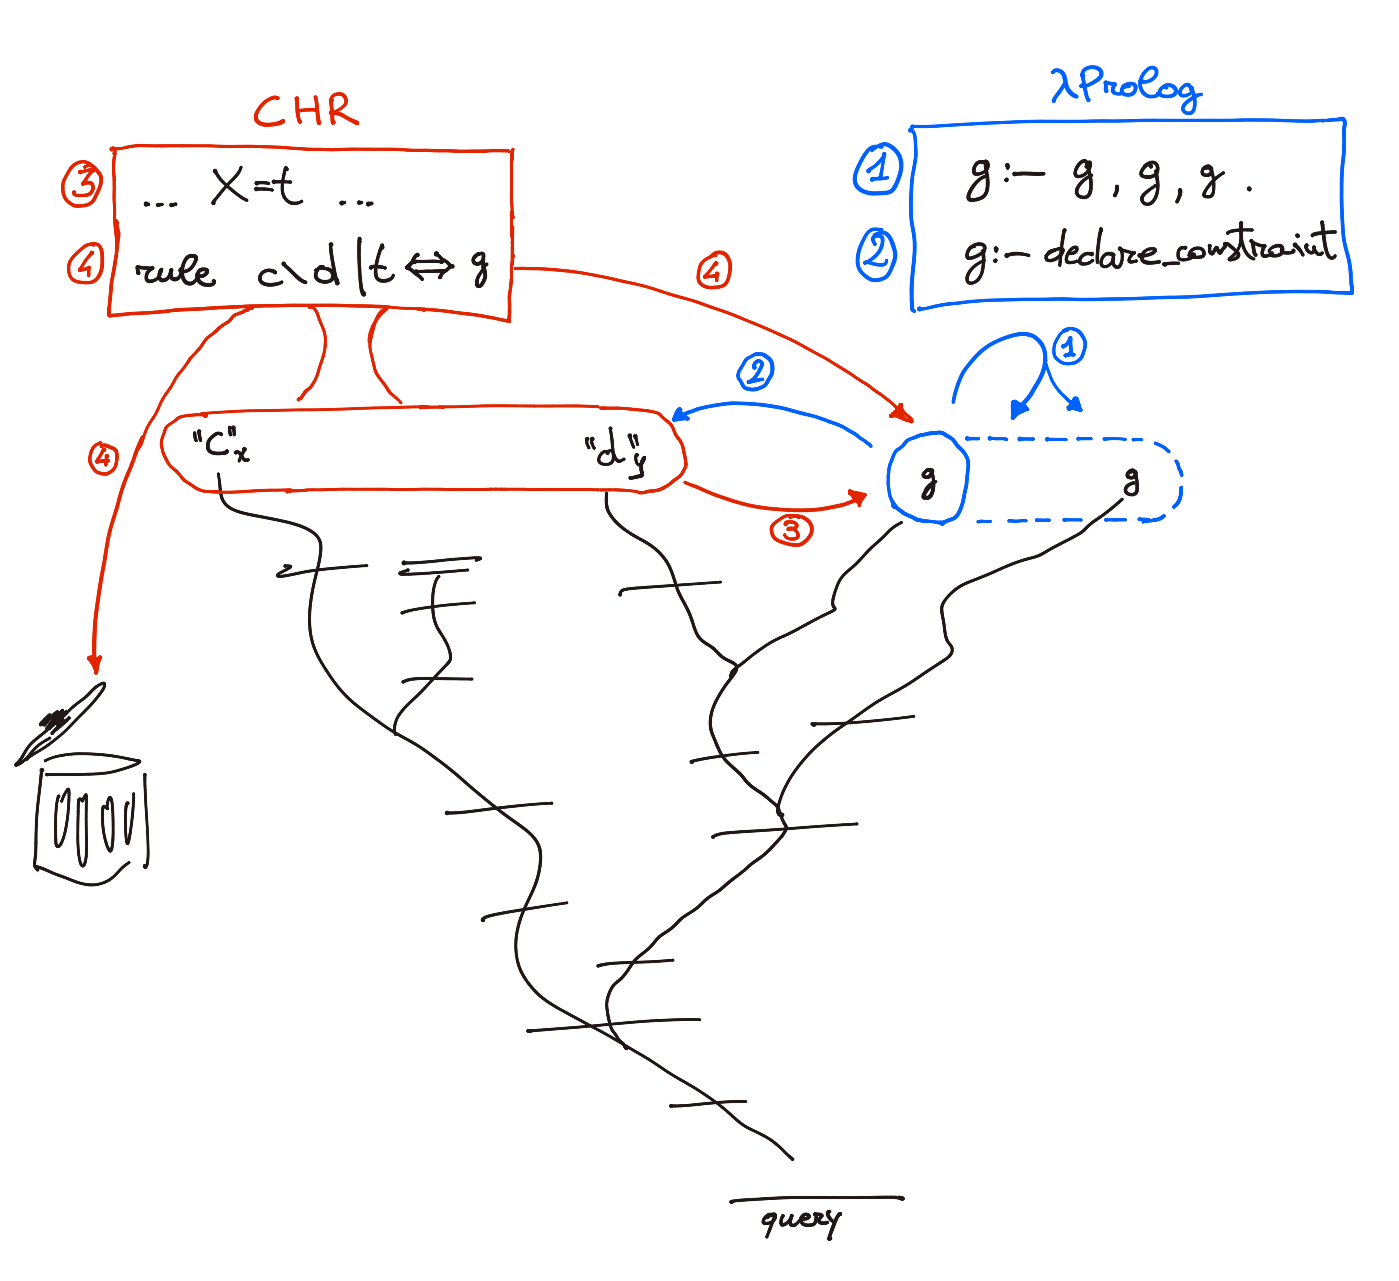
\includegraphics[width=0.9\textwidth]{chr.png}
    \caption{\label{fig:chr}An Elpi computation}
  \end{center}
\end{figure}

\newpage
\subsection{Abstract syntax and operational semantics}\label{sec:sem}

% The objective of this section is to act as a reference for
% the semantics of Elpi.

\newcommand{\vecL}[1]{\overrightarrow{\vphantom{t}#1}}
\newcommand{\BASE}{\ensuremath{\mathbb{B}}}
\newcommand{\PRED}[1][]{\ensuremath{\mathbb{F}#1}\xspace}
\newcommand{\VAR}[1][]{\ensuremath{\mathbb{V}#1}\xspace}
\newcommand{\APP}[1][]{\ensuremath{\mathbb{Ap}#1}\xspace}
% \def\CALL{\APP}
\newcommand{\X}[1][]{\ensuremath{\mathcal{X}#1}\xspace}
\newcommand{\T}[1][]{\ensuremath{tm#1}\xspace}
\newcommand{\V}[1][]{\ensuremath{\mathcal{V}#1}\xspace}
\newcommand{\CHR}[1][]{\ensuremath{\mathbb{C}#1}\xspace}
\newcommand{\CLAUSE}[1][]{\ensuremath{\mathbb{R}}#1\xspace}
\newcommand{\ATOM}[1][]{\ensuremath{\mathbb{A}#1}\xspace}
\newcommand{\A}[1][]{\ensuremath{\mathbb{A}#1}\xspace}
\newcommand{\Ainst}[1][]{\ensuremath{\alpha#1}\xspace}
\newcommand{\bool}[1][]{b}
\newcommand{\B}[1][]{\ensuremath{\mathrm{B}}\xspace}
\newcommand{\F}[1][]{\ensuremath{\mathbb{D}}\xspace}
\newcommand{\subst}[1][]{\ensuremath{\sigma#1}\xspace}
\newcommand{\alt}[1][]{\ensuremath{\mathcal{A}#1}\xspace}
\newcommand{\alts}[1][]{\ensuremath{a#1}\xspace}
\newcommand{\g}[1][]{\ensuremath{\mathcal{G}#1}\xspace}
\newcommand{\clause}[1][]{\ensuremath{\mathcal{@}#1}\xspace}
\newcommand{\pred}[1][]{\ensuremath{p#1}\xspace}
\newcommand{\expr}[1][]{\texttt{e#1}\xspace}
\newcommand{\vars}{\texttt{vars}}
\newcommand{\run}{\texttt{run}}
\newcommand{\fold}{\ensuremath{\mathbf{fold}}\xspace}
\newcommand{\map}{\ensuremath{\mathbf{map}}\xspace}
% \newcommand{\fail}{\texttt{fail}}
\newcommand{\call}{\texttt{Call}}
\newcommand{\cut}{\texttt{Cut}\xspace}
\newcommand{\cst}{\texttt{Cst}\xspace}
%\newcommand{\goal}{\texttt{Goal}}
\newcommand{\unifiable}{\texttt{unifiable}\xspace}
\newcommand{\matchable}{\texttt{matchable}\xspace}
\newcommand{\nUnify}{\texttt{split}\xspace}
\newcommand{\unify}{\texttt{unify}\xspace}
\newcommand{\match}{\texttt{match}\xspace}
\newcommand{\impl}{\texttt{=>}}
\newcommand{\prog}[1][]{\ensuremath{{\pi}#1}\xspace}
\newcommand{\pin}{\texttt{pi}}
\newcommand{\cdash}{\texttt{:-}} % colon-dash
\newcommand{\Cons}[1]{\ensuremath{#1::}}
\newcommand{\ConsHd}[1]{\ensuremath{(#1::}\xspace}
\newcommand{\ConsTl}[1]{\ensuremath{#1)}\xspace}
\newcommand{\EmptyList}{\ensuremath{\varnothing}}
\newcommand{\ConsHdNP}[1]{\ensuremath{#1::}\xspace}
\newcommand{\ConsTlNP}[1]{\ensuremath{#1}\xspace}

\newcommand{\EmptySubst}{\ensuremath{\varepsilon}}

\newcommand{\PROG}[1][]{\ensuremath{\mathcal{P}#1}\xspace}
\newcommand{\progCut}{\ensuremath{\prog[^!]}\xspace}
\newcommand{\evdash}{\ensuremath{\colondash}\xspace}
\newcommand{\piimpl}{{\ensuremath{\forall\Rightarrow}}\xspace}
\newcommand{\TYPE}[1][]{\ensuremath{\mathbb{T\!y}#1}}
\newcommand{\TERM}[1][]{\ensuremath{\mathbb{T\!m}#1}}
\newcommand{\SIGN}[1][]{\ensuremath{\mathbb{S}#1}}
\newcommand{\func}[1][]{\ensuremath{\mathcal{D}#1}}
\newcommand{\implCmd}[2]{\ensuremath{#1\ \impl\ #2}}
\newcommand{\bchain}{\ensuremath{\mathcal{B}}}
\newcommand{\cselect}{\ensuremath{\mathcal{U}}}
% \newcommand{\bs}{\text{\textbackslash}}
\newcommand{\bs}{\text{.}}
\newcommand{\piCmd}[2]{\ensuremath{\pin\ #1 \bs\ #2}}
% \newcommand{\piImplCmd}[3]{\piCmd{#1}{\implCmd{#2}{#3}}}
\newcommand{\ground}{\texttt{ground}}
\newcommand{\dom}{\texttt{vars}}
\newcommand{\clauseCmd}[3]{\ensuremath{#1\ #2\ \cdash\ #3}}
\newcommand{\atsign}{\ensuremath{\mbox{\footnotesize\raisebox{-1pt}{\ensuremath{@}}}}}
\newcommand{\Keyword}[1]{\texttt{{\fontfamily{qcr}\selectfont #1}}}
\newcommand{\kIF}{\Keyword{if}}
\newcommand{\kTHEN}{\Keyword{then}}
\newcommand{\kELSE}{\Keyword{else}}
\newcommand{\kAS}{\Keyword{as}}

\paragraph{Conventions}
We write \(\vecL{t}\) to denote \(t_1 \ldots t_n\) i.e. a (possibly
empty) list of \(t\)s.
Similarly, we write \(\vecL{tu}\) to denote the
element-wise pairing (zipping) of \(\vecL{t}\) and \(\vecL{u}\) into a list of
pairs. %The zipping process continues up to the length of the shorter list.
% \todo{check for dead cod here if we hide the proofs}
Finally write
$t[x/y]$ for the usual, capture avoiding, operation of replacing the variable $x$
with $y$ inside $t$.

We use $\EmptyList$ for the empty list and $x :: xs$ for prepending an element $x$
to a list $xs$; $\atsign$ for list concatenation;
$[e\ \kIF\ p\ |\ x \in \vec{x}]$ for list comprehension (we omit the filter when $p$ is true).

We denote with $\_\times\_$, $\_+\_$, $\vecL{\phantom{i}\_~}$ and $\_\to\_$ the product, disjoint union, list and
function space of types, respectively, and with $\B = \{ \top, \bot\}$ the booleans.
By abuse of notation we use non-terminals as types, i.e., $\mathbb{A}$
is the type of atoms.
% We omit the conversion between the (isomorphic) types $A \times B \to C$
% and $A \to B \to C$, e.g. we may write $\map\ f\ \vecL{tu}$ instead of $\map\ (\lambda x.f\ (\text{fst}\ x)\ (\text{snd}\ x))\ \vecL{tu}$.

\paragraph{Syntax}
The abstract syntax of Elpi is given in~\cref{fig:syntax}.
We assume a set \PRED of functors (term/predicate constructors), and a set \VAR of term variables
($X,Y,\ldots$ for unification variables and $x,y,\ldots$ for bound variables).
% The non-terminal \CALL groups callable symbols ($c,d,\ldots$): either predicate names or variables.

In the syntax of atoms \ATOM we single out \cut and \cst.
The \cut operator corresponds to \elpi{!} in the concrete syntax.
The \cst one corresponds to \elpi{declare_constraint} in the concrete syntax
and it carries the applicative term to suspend and the list of variables triggering
its resumption.
In the syntax for constraint rules \CHR we find first a list of
terms representing patterns to match, then a list of terms to match and remove,
then a guard\footnote{The guard defaults to the always true one in the concrete syntax}
and finally a list of new goals.

%The non-terminal $\TERM$, for terms, includes predicate calls, functor applications and $\lambda$-abstraction.
% For simplicity we glue together the
% \elpi{pi} and \elpi{=>} in the same grammar production and we
% rule out predicates inside data (like lists of predicates).

%for regular data or \V{} for 
% and polymorphic data.
% We note $\Ainst \in \A$.
% The usual =/2 operator is
% encoded as a regular predicate \texttt{eq} with a single clause
% \elpi{(eq X X :- .)} and signature\todo{dire che poly è solo su exp}
% $\ctx\ \texttt{eq} = \dtype{\detI}{}{\expI\ \expI}$: a deterministic predicate\todo{should add var to static check}
% with two outputs of the same type.

% We say that $\vars\ t$ is the set
% of free variables occurring in $t$ (the binders are \elpi{pi} and $\lambda$).
% When $\vars\ t = \EmptyList$ we say that
% $t$ is \ground.

% We call \emph{toplevel clauses} the ones that are in the initial program.
% %or equivalently that are asserted by the atoms in the query. 
% We call
% \emph{hypothetical clauses} the ones that are asserted by atoms in the premises
% of a clause.

\begin{figure}
  $$
  \begin{array}{rlr}
    \PRED & ::= p, q, \ldots, f, g, \ldots & \mathrm{functors}\\
    \VAR & ::= \mathrm{X}, \mathrm{Y} \ldots x, y, \ldots & \mathrm{variable}\\
    \APP & ::= \PRED\ \vecL{\TERM} \mid  \VAR\ \vecL{\TERM} & \mathrm{applicative}\\
    \ATOM& ::= \cut \mid \cst\ \APP\ \vecL{\VAR} \mid \APP \mid \piCmd{\VAR}{\ATOM} \mid \implCmd{{\CLAUSE}}{\ATOM} & \mathrm{atom} \\
    \TERM & ::= \APP \mid \lambda \VAR \bs\ \TERM & \mathrm{term}\\
    \CLAUSE & ::= \clauseCmd{\APP}{\!}{\vecL{\ATOM}} & \mathrm{logic\ programming\ rule}\\
    \CHR & ::= \vecL{\APP}\ \backslash\ \vecL{\APP}\ 
               \mathrm{|}\ \APP \Leftrightarrow  \vecL{\APP} & \mathrm{constraint\ rule}
  \end{array}
  $$
  \caption{Abstract syntax}
  \label{fig:syntax}
\end{figure}

\newenvironment{myRule}[1]{%
  \begin{minipage}{.9\textwidth}
    \centering
    \begin{prooftree}%
      } % Here will be put the body
      {
    \end{prooftree}
    \vspace{2pt}
  \end{minipage}
}
\newcommand{\arr}{\ensuremath{\rightsquigarrow}}
\makeatletter
\newcommand{\customlabel}[2]{%
  \protected@write \@auxout {}{\string \newlabel {#1}{{\ensuremath{#2}}{\thepage}{#2}{#1}{}} }%
  \hypertarget{#1}{\ensuremath{#2}}
}
\makeatother
\newcommand{\runCmdR}[3]{\ensuremath{\run\ (k,\ #3,\ #1)\ #2 \arr r}}
\newcommand{\runCmdRK}[4]{\ensuremath{\run\ (#4,\ #3,\ #1)\ #2 \arr r}}
\newcommand{\runCmd}[7]{\ensuremath{\run\ (#4,\ #3,\ #1)\ #2 \arr (#7,\ #6,\ #5)}}
%\newcommand{\runCmdQ}[4]{\ensuremath{\run\ #1\ #2 \arr (#3, #4)}}
\newcommand{\runCmdQR}[2]{\ensuremath{\run\ #1\ #2 \arr r}}
\newcommand{\runQuery}[2]{\ensuremath{\run\ (\EmptySubst,\ \EmptySubst,\ #1)\ #2 \arr \_}}
\newcommand{\runCmdF}[3]{\ensuremath{\run\ (k,\ #3,\ #1)\ #2 \arr \bot}}
% \newcommand{\callCmd}[3]{\ensuremath{(\call\ #1\ #2\ #3)}\xspace}
\newcommand{\callCmd}[2]{\ensuremath{(#1\ #2)}\xspace}
\newcommand{\goalCmd}[3]{\ensuremath{(#1,\ #2,\ #3)}\xspace}
\newcommand{\ruleName}[2]{\customlabel{#1}{\ensuremath{\mathrm{run}_{#2}}}}
\newcommand{\RightLabelM}[1]{\RightLabel{\scriptsize #1}}

\newcommand{\ruleFail}{\ruleName{rule:backtrack}{\circlearrowright }}
\newcommand{\ruleAbort}{\ruleName{rule:abort}{\bot}}
\newcommand{\ruleCall}{\ruleName{rule:call}{@}}
\newcommand{\ruleCallF}{\ruleName{rule:callbacktrack}{\circlearrowright}}
\newcommand{\ruleCallFH}{\ruleName{rule:callabort}{\bot}}
% \newcommand{\ruleCallB}{\ruleName{rule:call1}{@'}}
\newcommand{\ruleBeta}{\ruleName{rule:beta}{\sigma}}
\newcommand{\ruleBang}{\ruleName{rule:cut}{!}}
\newcommand{\ruleCst}{\ruleName{rule:delay}{\bigtriangleup}}
\newcommand{\ruleTcs}{\ruleName{rule:resume}{\bigtriangledown}}
% \newcommand{\ruleCHR}{\customlabel{rule:chr}{\ensuremath{\mathrm{run}_*}}}
\newcommand{\ruleStop}{\ruleName{rule:stop}{\top}}
\newcommand{\ruleUnif}{\ruleName{rule:unif}{=}}
\newcommand{\ruleImpl}{\ruleName{rule:impl}{\Rightarrow}}
\newcommand{\rulePi}{\ruleName{rule:pi}{\forall}}
\newcommand{\ruleMatch}{\ruleName{rule:match}{m}}
\newcommand{\rulePiImpl}{\ruleName{rule:piimpl}{{\piimpl}}}

\newcommand{\ruleStopM}[1]{
  \begin{myRule}{#1}
    % STOP
    \AxiomC{\vspace{2em}\phantom{\ensuremath{\bchain}}}
    \RightLabelM{\ruleStop}
    \UnaryInfC{\runCmd{\EmptyList}{\alts}{\subst}{\kappa}{\alts}{\subst}{\kappa}}
  \end{myRule}
}

% \newcommand{\ruleUnifM}[1]{
%   \begin{myRule}{#1}
%     % UNIF
%     \AxiomC{\unifyCmd{x}{y}{\subst}{\subst[']}}
%     \AxiomC{\runCmdR{\vecL{g}}{\alts}{\subst[']}}
%     \RightLabelM{\ruleUnif}
%     \BinaryInfC{\runCmdR{\ConsHdNP{\goalCmd{\_}{x = y}{\_}}\ConsTlNP{\vecL{g}}}{\alts}{\subst}}
%   \end{myRule}
% }

% \newcommand{\ruleMatchM}[1]{
%   \begin{myRule}{#1}
%     % MATCH
%     \AxiomC{\matchCmd{x}{y}{\subst}{\subst[']}}
%     \AxiomC{\runCmd{\vecL{g}}{\alts}{\subst[']}{\alts[']}{\subst['']}}
%     \RightLabelM{\ruleMatch}
%     \BinaryInfC{\runCmd{\ConsHdNP{\goalCmd{\_}{(x =_m y)}{\_}}\ConsTlNP{\vecL{g}}}{\alts}{\subst}{\alts[']}{\subst['']}}
%   \end{myRule}
% }

\newcommand{\ruleFailM}[1]{
  \begin{myRule}{#1}
    % FAIL
    \AxiomC{\unifyCmd{x}{y}{\subst}{\bot}}
    \AxiomC{\runCmdQR{\alts}{al}}
    \RightLabelM{\ruleFail}
    \BinaryInfC{\runCmdR{\ConsHdNP{\goalCmd{\_}{x = y}{\_}}\ConsTlNP{\_}}{\ConsHd{\alts}\ConsTl{al}}{\subst}}
  \end{myRule}%
}

\newcommand{\ruleAbortM}[1]{
  \begin{myRule}{#1}
    % FAIL
    \AxiomC{\unifyCmd{x}{y}{\subst}{\bot}}
    \RightLabelM{\ruleAbort}
    \UnaryInfC{\runCmdF{\ConsHdNP{\goalCmd{\_}{x = y}{\_}}\ConsTlNP{\_}}{\EmptyList}{\subst}}
  \end{myRule}%
}

\newcommand{\ruleBangM}[1]{
  \begin{myRule}{#1}
    % CUT
    \AxiomC{\runCmdR{\vecL{g}}{\alts}{\subst}}
    \RightLabelM{\ruleBang}
    \UnaryInfC{\runCmdR{\ConsHdNP{\goalCmd{\_}{\cut}{\alts}}\ConsTlNP{\vecL{g}}}{\_}{\subst}}
  \end{myRule}
}
\newcommand{\ruleCstM}[1]{
  \begin{myRule}{#1}
    % suspend
    \AxiomC{\ensuremath{\mathcal{CHR}(k,\ \prog,\ \subst\ c,\ t,\ \alts[']) = (\vecL{g'}, k')}}
    \AxiomC{\runCmdRK{\vecL{g'} \atsign \vecL{g}}{\alts}{\subst}{k'}}
    \RightLabelM{\ruleCst}
    \BinaryInfC{\runCmdRK{\ConsHdNP{\goalCmd{\prog}{\cst\ c\ t}{\alts[']}}\ConsTlNP{\vecL{g}}}{a}{\subst}{k}}
  \end{myRule}
}
\newcommand{\ruleTcsM}[1]{
  \begin{myRule}{#1}
    % resume
    \AxiomC{
      \ensuremath{
        \begin{array}{c}
      (\prog,\ c,\ t) \in k \quad \exists v \in t, v \in \dom\ \subst\\
      \runCmdRK{\ConsHdNP{(\prog,\ c,\ a)}\vecL{g}}{\alts}{\subst}{k - (\prog,\ c,\ t)}
        \end{array}
      }
    }
    \RightLabelM{\ruleTcs}
    \UnaryInfC{\runCmdRK{\vecL{g}}{a}{\subst}{k}}
  \end{myRule}
}
% \newcommand{\ruleCHRM}[1]{
%   \begin{myRule}{#1}
%     % CHR
%     \AxiomC{\ensuremath{\mathcal{CHR}\ m = (\vecL{g'}, m')}}
%     \AxiomC{\runCmdR{\vecL{g'} \atsign \vecL{g}}{\alts}{(s,m')}}
%     \RightLabelM{\ruleCHR}
%     \BinaryInfC{\runCmdR{\vecL{g}}{\alts}{(s,m)}}
%   \end{myRule}
% }

\newcommand{\ruleCallM}[1]{
  \begin{myRule}{#1}
    % CALL
    \AxiomC{$\bchain(k,\ \prog,\ \pred\ \vecL{t},\ \vecL{g},\ \subst,\ al) = \ConsHdNP{\alts[']}\ConsTlNP{al'}$}
    \AxiomC{\runCmdQR{\alts[']}{(al'\ \atsign\ al)}}
    \RightLabelM{\ruleCall}
    \BinaryInfC{\runCmdR{\ConsHdNP{\goalCmd{\prog}{\callCmd{\pred}{\vecL{t}}}{\_}}\ConsTlNP{\vecL{g}}}{al}{\subst}}
  \end{myRule}
}
\newcommand{\ruleCallMF}[1]{
  \begin{myRule}{#1}
    % CALL
    \AxiomC{$\bchain(k,\ \prog,\ \pred\ \vecL{t},\ \vecL{g},\ \subst,\ a::al) = \EmptyList$}
    \AxiomC{\runCmdQR{a}{al}}
    \RightLabelM{\ruleCallF}
    \BinaryInfC{\runCmdR{\ConsHdNP{\goalCmd{\prog}{\callCmd{\pred}{\vecL{t}}}{\_}}\ConsTlNP{\vecL{g}}}{(a :: al)}{\subst}}
  \end{myRule}
}
\newcommand{\ruleCallMFH}[1]{
  \begin{myRule}{#1}
    % CALL
    \AxiomC{$\bchain(k,\ \prog,\ \pred\ \vecL{t},\ \vecL{g},\ \subst,\ \EmptyList) = \EmptyList$}
    \RightLabelM{\ruleCallFH}
    \UnaryInfC{\runCmdF{\ConsHdNP{\goalCmd{\prog}{\callCmd{\pred}{\vecL{t}}}{\_}}\ConsTlNP{\vecL{g}}}{\EmptyList}{\subst}}
  \end{myRule}
}

\newcommand{\ruleCallBeta}[1]{
  \begin{myRule}{#1}
    \AxiomC{$\subst (X\ \vecL{t}) =_{\beta\eta} \pred\ \vecL{u}$}
    \AxiomC{\runCmdR{\ConsHdNP{\goalCmd{\prog}{\pred\ \vecL{u}}{a}}\ConsTlNP{\vecL{g}}}{\alts[']}{\subst}}
    \RightLabelM{\ruleBeta}
    \BinaryInfC{\runCmdR{\ConsHdNP{\goalCmd{\prog}{(X\ \vecL{t})}{a}}\ConsTlNP{\vecL{g}}}{\alts[']}{\subst}}
  \end{myRule}
}


% \newcommand{\ruleCallBM}[1]{
%   \begin{myRule}{#1}
%     % CALLB
%     \AxiomC{$(\subst h)\ \vecL{t} =_\beta \pred\ \vecL{u}$}
%     \AxiomC{$\bchain(\prog, \pred\ \vecL{u}, \subst, \alts) = \ConsHdNP{g}\ConsTlNP{new\_alt}$}
%     \AxiomC{\runCmdR{(g\ \atsign\ \vecL{g})}{(new\_alt\ \atsign\ \alts)}{\subst}}
%     \RightLabelM{\ruleCallB}
%     \TrinaryInfC{\runCmdR{\ConsHdNP{\goalCmd{\prog}{(h\ \vecL{t})}{\_}}\ConsTlNP{\vecL{g}}}{\alts}{\subst}}
%   \end{myRule}
% }

\newcommand{\env}{\ensuremath{\mathcal{E}}}

\newcommand{\ruleImplM}[1]{
  \begin{myRule}{#1}
    % IMPL
    \AxiomC{\ensuremath{\runCmdR{\ConsHdNP{\goalCmd{(h + \prog)}{g}{\alts}}\ConsTlNP{\vecL{g}}}{\alts[']}{\subst}}}
    \RightLabelM{\ruleImpl}
    \UnaryInfC{\ensuremath{\runCmdR{\ConsHdNP{\goalCmd{\prog}{(\implCmd{h}{g})}{\alts}}\ConsTlNP{\vecL{g}}}{\alts[']}{\subst}}}
  \end{myRule}
}

\newcommand{\rulePiM}[1]{
  \begin{myRule}{#1}
    % PI
    \AxiomC{\ensuremath{y \# \prog \quad \runCmdR{\ConsHdNP{\goalCmd{(y + \prog)}{g[x/y]}{\alts}}\ConsTlNP{\vecL{g}}}{\alts[']}{\subst}}}
    \RightLabelM{\rulePi}
    \UnaryInfC{\ensuremath{\runCmdR{\ConsHdNP{\goalCmd{\prog}{(\piCmd{x}{g})}{\alts}}\ConsTlNP{\vecL{g}}}{\alts[']}{\subst}}}
  \end{myRule}
}

% \newcommand{\rulePiImplM}[1]{
%   \begin{myRule}{#1}
%     % IMPL
%     \AxiomC{$y \# \prog$}
%     \AxiomC{\runCmdR{\ConsHdNP{\goalCmd{(y,h[y/x]) + \prog}{g[y/x]}{\alts}}\ConsTlNP{\vecL{g}}}{\alts[']}{\subst}}
%     \RightLabelM{\rulePiImpl}
%     \BinaryInfC{\runCmdR{\ConsHdNP{\goalCmd{\prog}{(\piCmd{x}{\implCmd{h }{g}})}{\alts}}\ConsTlNP{\vecL{g}}}{\alts[']}{\subst}}
%   \end{myRule}
% }


\newcommand{\unifyCmd}[5][]{\ensuremath{
  \ifstrequal{#1}{1}
    {\vecL{\unify\ #2\ #3}}
    {\unify\ #2\ #3}\ #4 = #5}}
\newcommand{\matchCmd}[5][]{\ensuremath{
  \ifstrequal{#1}{1}
  {\vecL{\match\ #2\ #3}}
  {\match\ #2\ #3}\ #4 = #5}}

\paragraph{Semantics}

A substitution $\subst$ of type $\Sigma$
%is a pair $(s,m)$ where $s$ 
is a partial mapping from unification variables
\VAR to terms \TERM{}. % and $m$ is a constraint store.
We write
% $s\ t$ the application of the substitution $s$ to a term $t$, and 
$\subst\ t$ the  application of the substitution to $t$.
%the first component of \subst to $t$.
% ,
% and we remark that $t$ is \ground{} iff $\forall \subst, \subst t = t$.
We write $\dom\ \subst$ for the set of variables occurring
in the domain %or in the codomain 
of \subst, i.e.
$\dom\ \subst = \{\ X\ |\ \subst X \mathrm{\ is\ defined\ }\}$. % \lor X \in \vars\ (\subst Y) \mathrm{\ for\ some\ Y} \}$.
The empty substitution is written $\EmptySubst$. % is so that $\dom\ \EmptySubst = \EmptyList$.

We assume a function $\unify$ of type $\TERM \times \TERM \times \Sigma \to \Sigma + \bot$
such that if $\unifyCmd{t_1}{t_2}{\subst}{\subst[']} \not= \bot$ 
then \subst['] is the most general extension of \subst 
such that $\subst['] t_1 = \subst['] t_2$~\cite{miller92jsc}.
We assume a function $\match$ of type $\TERM \times \TERM \times \Sigma \to \Sigma + \bot$
such that if $\matchCmd{t}{p}{\subst}{\subst[']} \not= \bot$
then \subst[']  is the most general extension of  $\subst$
such that $\subst['] p = \subst t$ and $\subst[']t = \subst t$,
i.e. \match{} does not assign variables in $t$ but only in $p$ that acts as the pattern.

A program $\prog$ of type $\PROG$ is a pair $(\mathbb{N}, \mathcal{I})$
where $\mathbb{N}$ is a set of names and $\mathcal{I}$ an index
mapping predicate names to an \emph{ordered list} of rules.
We write $x \# \prog$ to find a name fresh in $\mathbb{N}$.
We write $\prog~\pred$ for the rules of predicate \pred in $\mathcal{I}$
and we write $x + \prog$ to add the name $x$ to $\mathbb{N}$
and we write $h + \prog$ to prepend the extra rules $h$  to $\mathcal{I}$
(hence $h$ has the highest priority in the new program).


A constraint store $\kappa$ of type $K = \vecL{\PROG \times \APP \times \vecL{\VAR}}$
is a multiset of triples $(\prog,c,t)$
where $\prog$ is a program, where $c$ stands for a constraint (an applicative term in $\APP$) and $t$
of type $\vecL{\VAR}$ is the trigger. The empty store is written $\EmptySubst$;
we use $k - (\prog,c,t)$ to remove a constraint from the store.
The rules acting on the constraint store $\mathcal{R = \vecL{\mathbb{C}}}$ are
morally part of the program, but since they never change we omit them.


A goal $g$ of type $\g = \PROG \times \ATOM \times \vecL{\alt}$
is a triple made of a program, an atom and a list of
so called \emph{cut-to} alternatives.
An alternative $a$ of type $\alt$ is a triple of type $K \times \Sigma \times \vecL{\g}$
made of a constraint store, a substitution and a list of goals.

\begin{figure}[p]
    \centering

  % \ruleCHRM{.4}
  \ruleTcsM{.4}
  \ruleCstM{.4}
  \caption{Semantics: constraints}
    \label{fig:basic-interp-c}
\end{figure}

  \begin{figure}[p]
  \centering
  \ruleStopM{.37}
  \ruleCallMFH{0.44}
  \ruleCallMF{0.58}
  % \vspace{0.3em}%
  \ruleBangM{.4}
  \ruleCallM{1}
%


  \rulePiM{1}
  \ruleImplM{1}
  \ruleCallBeta{1}
  
  \caption{Semantics: higher-order logic programming}
    \label{fig:basic-interp-l}
\end{figure}



The operational, big-step semantics of Elpi is defined by the function
$$
\run{} : \alt \times \vecL{\alt} \to (K  \times \Sigma \times \vecL{\alt}) + \bot
$$
shown in Figures~\cref{fig:basic-interp-c} and~\cref{fig:basic-interp-l}.
We write \runCmd{\vecL{g}}{a}{\subst}{\kappa}{a'}{\subst'}{\kappa'}
to indicate that a goal list $\vecL{g}$ in a constraint store $\kappa$, under a
substitution $\subst$ and alternatives $a$, terminates with an updated
constraint store $\kappa'$, a substitution $\subst'$, and a remaining list of
(still unexplored) alternatives $a'$. We write \runCmdF{\vecL{g}}{a}{\subst}
when the execution halts, that is, when it fails to solve one of the given goals
and runs out of alternatives.
%An initial query looks like \runQuery{[\goalCmd{\prog}{\pred\ \vecL{t}}{\EmptyList}]}{\EmptyList}

The rules in~\cref{fig:basic-interp-l} are syntax directed, while the ones
in~\cref{fig:basic-interp-c} are given top priority and are applied in order. 
Even if rules for CHR have precedence we start by explaining the ones
in~\cref{fig:basic-interp-l} because they give a meaning to the cut-to
alternatives.

Rule~\ref{rule:stop} applies when all goals are solved and returns the
constraint store and the
substitution along with the still unexplored alternatives. Rule~\ref{rule:callabort}
applies when no rule matches the current goal and no alternative is available.
Rule~\ref{rule:callbacktrack} implements (chronological) backtracking by simply
popping the first alternative, returning to the most recent choice point.\footnote{A
choice point is, intuitively, an anchor to a point in time we could backtrack to.
When doing so assignments are undone, discarding the result of the failed computation.}
\index[concepts]{Choice point}
Rule~\ref{rule:cut} implements a hard cut by restoring the cut-to alternatives
saved by $\bchain$ (see its description below). Rule~\ref{rule:call} backchains
all applicable rules, generating new alternatives, the first of which becomes
the new goal. Rule~\ref{rule:beta} accounts for the higher-order programming
aspect of $\lambda$Prolog: unification variables can be used to pass predicates
around. For example \elpi{P = true, P} is a query that requires Rule~\ref{rule:beta}
to succeed.
Rule~\ref{rule:pi} introduces a fresh name into the program, while
Rule~\ref{rule:impl} introduces a new rule into the program.

Rules~\ref{rule:delay} and~\ref{rule:resume}
address the constraint aspect of the language: the former updates the constraint
store when a new constraint is declared, while the latter resumes a constraint
as soon as the substitution $\subst$ acts on its trigger. The second rule
follows~\cite{Michaylov1993HigherOrderLP}, which also investigates how to
combine higher-order logic programming with constraint programming. It may look
wrong that the rule
uses the current alternatives as the cut-to alternatives for the resumed goal,
but these cut-to alternatives will never be used since constraints are
applicative terms, i.e., not the cut operator.

\paragraph{Definition of $\bchain$ (backchain)}\label{backchain}

The role of $\bchain$ of type $K \times \mathcal{P} \times \APP \times \vecL{\g} \times \Sigma \times \vecL{\alt} \to \vecL{\alt}$ is to generate
an alternative for each rule that applies to the given goal.

  $$
  \begin{array}{l}
    \vspace{1em}
  \bchain(k,\ \prog,\ \pred\, \vecL{t},\ \vecL{g},\ \subst,\ a) =\\
  \quad
  \bigg[
    \underbrace{
      (k,\ 
      \subst['],\ 
      \big(\big[(\prog, g, a) \mid g \in\! \vecL{b}\big]\ \atsign\ \vecL{g}\big))
    }_{
      \mathrm{of~type}~\mathcal{A}
    }
    \ \kIF\ \cselect(\vecL{tu},\ \subst) = \subst['] \not= \bot
    ~\bigg|\\
    \hspace{23em}
    \underbrace{(\clauseCmd{\pred}{\vecL{u}}{\vecL{b}})}_{\mathrm{of~type~}\mathbb{R}} \in \prog\ \pred
    \bigg]\vspace{1em}
  \end{array}
  $$

It is worth noting that each new goal (in each alternative) carries the same
cut-to alternative $a$, and that the value passed to $\bchain$ by rule
\ref{rule:call} is the list of alternatives prior to backchaining. In other
words, it does not include any alternatives being created, nor any that will be
created in the future by exploring the new alternatives.

\paragraph{Definition of $\cselect$ (select)}

The function $\cselect$ is used to filter rules, retaining only those that
apply. Unlike standard Prolog, arguments marked by the user as input (denoted
$\vecL{tu_i}$) are matched, while those marked as output (denoted
$\vecL{tu_o}$) are unified.

  $$
  \begin{array}{l}
  \cselect(\vecL{tu}, \subst) = \fold\ \unify\ \vecL{tu_o}\ (\fold\ \match\ \vecL{tu_i}\ \subst)
  \end{array}
  $$

The list processing combinator \fold is defined by the following equations:
$$
\begin{array}{lll}
\fold\ \_\ \_\ \bot = \bot & \quad\fold\ f\ (x :: xs)\ a = \fold\ f\ xs\ (f\ x\ a) & \quad\fold\ \_\ \EmptyList\ a = a
\end{array}
$$

\paragraph{Definition of $\mathcal{CHR}$ (simpagation)}
 
CHR rules do have a logical reading. 
In particular a rule $G_1\ \backslash\ G_2\ |\ T \Leftrightarrow G_3$
is to be understood as $T \land G_1 \Rightarrow (G_2
\Leftrightarrow G_3)$: when the guard $T$ holds, we can replace $G_2$ by $G_3$
provided that $G_1$ still needs to be solved.

Constraint rule application in Elpi follows the refined operational
semantics~\cite{10.1007/978-3-540-27775-0_7}, which amounts to a precise
nesting of iterations.
The starting point is the so-called \emph{active constraint}, which, in the context
of Elpi, is the constraint just declared as $\cst\ c\ t$ by rule~\ref{rule:delay}.
\index[concept]{Active constraint}

$$
\mathcal{CHR}(k,\ \prog,\ c,\ t,\ \alts) = (g', k')\ \mathrm{where}
$$
\begin{enumerate}
\item add the active constraint $(\prog,\ c,\ t)$ to $k$ to obtain $k'$, and set $g'$ to $\EmptyList$
\item for each rule $P_1 \ldots P_x\ \backslash\ P_{x+1} \ldots P_n\ |\ Q \Leftrightarrow G$
\item for each position $0 < j \leq n$ in increasing order
\item for each permutation of $C_1 \ldots C_n$ constraints in $k'$ having $C_j = (\prog,\ c,\ t)$ ($C_j$ is
the active constraint)
\item match all $C_i$ with $P_i$ and run the guard $Q$ in the initial program $\pi_0$.
  If the guard succeeds, i.e., $\runCmd{[\pi_0,Q,\EmptyList]}{\EmptyList}{\EmptySubst}{\EmptyList}{\_}{\subst}{\EmptyList}$, then:
  \begin{itemize}
    \item remove $C_{x+1} \ldots C_n$ from $k'$
    \item remove all permutations involving $C_{x+1} \ldots C_n$
    \item add $\subst G$ to $g'$
  \end{itemize}
\item move to the next rule (point 2)
\end{enumerate}


 As
anticipated in~\cref{sec:modes}, adapting CHR to Elpi -- or more precisely, to its
$\lambda$Prolog part -- requires some extra care. In particular, a constraint
$((\mathbb{N},\mathcal{I}),\ c,\ t)$ represents a $\lambda$Prolog goal:
$$
\mathbb{N} \triangleright  \mathcal{I} \vdash c
$$
where $\mathbb{N}$ is the set of nominal constants introduced by \elpi{pi}, and
$\mathcal{I}$ is the set of rules available to solve $c$. Pragmatically, only
hypothetical rules are stored in the constraint, since all static rules are
common to all constraints.

For simplicity, the context $\mathcal{I}$ is presented as a list: if the user
wants to compare these contexts as sets, they must implement the quotienting
in the rule's guard $Q$. To simplify context management, the user can specify a
filter to discard hypothetical rules for predicates not relevant to the constraint
(typically, rules for predicates unrelated to $c$). For reference, the concrete
syntax for a block of rules about constraints \elpi{p} and \elpi{q} under a
context restricted to \elpi{r} and \elpi{s} is:

\begin{elpicode}
constraint r s ?- p q {
  % rules for sequents on p or q under p, q, r and s
}
\end{elpicode}
\noindent
Once more, pragmatically, unless the user explicitly opts out, step 4 only
considers permutations of constraints with a trigger that overlaps with the
trigger $t$ of the active constraint.
This lets the user group constraints into clusters,
drastically reducing the number of permutations
to consider. In order to opt out the user can add a designated, inert,
trigger to all constraints as follows:
\begin{elpicode}
code :- declare_constraint (p X) [X, _].
%                                    ^ special trigger
\end{elpicode}
The special trigger \elpi{_} is a designated, unnamed variable. It cannot be
assigned, so it plays no role as a trigger. In the example above, the trigger
\elpi{[X, _]} is equivalent to \elpi{[X]} with respect to~\ref{rule:resume},
but it is common to all triggers that specify it when computing whether two
triggers overlap; i.e., \elpi{[X, _]} and \elpi{[Y, _]} do overlap.

Finally, the system enforces the disjointness of names used in each constraint;
that is, step 1 really adds $((\mathbb{N'},\mathcal{I'}),\ c',\ t)$ to $k$,
where each name in $\mathbb{N'}$ is fresh in $k$, and where $\mathcal{I'}$ and
$c'$ are obtained by substituting each name in $\mathbb{N}$ with the
corresponding one in $\mathbb{N'}$.

We refer the interested reader to~\cite{TASSI_2019} for a more formal
description of the operational semantics of the $\mathcal{CHR}$ procedure.

\subsection{Constraints v.s. global variables}

Most programming languages, including variants of Prolog, offer the concept of
global variables -- a feature that, while best used sparingly, can be extremely
convenient. Elpi does not natively support global variables, but it is easy to
implement a global state on top of constraint handling rules, provided that the
read/write performance of global variables is not critical for the application.


Here is an example of an integer global variable with a set/get API.

\begin{elpicode}
pred set i:int.
set I :- declare_constraint (set I) [_].

pred get o:int.
get I :- declare_constraint (get I) [_].

pred value i:int.
value I :- declare_constraint (value I) [_].

constraint set get value {
  rule \ (set I) (value _)   <=> (value I).           
  rule (value J) \ (get I)   <=> (I = J).      
  rule (set _)               <=> (halt "no global variable").
  rule (get _)               <=> (halt "no global variable").
  rule (value _) (value _)   <=> (halt "double initialization").
}
\end{elpicode}

The code uses \elpi{value} to initialize the global variable, and
\elpi{set} or \elpi{get} to overwrite or read its value.

\begin{elpioutput}
goal> value 2, get N, set 3.

Success:
  N = 2

Constraints:
 value 3  /* suspended on X0 */
\end{elpioutput}

Note that the constraint store honors backtracking, making this global state
simply a convenient way to avoid threading an explicit state, as one would do
in a pure language.

\newpage
\section{Syntactic sugar}


Elpi features some simple syntactic sugar that is eliminated by the compiler (see~\cref{sec:compiler})
before running programs.

\subsection{Namespaces}

Elpi programs are constructed by accumulating files -- that is, by concatenating lists
of rules, which may be written by different authors. It is possible for two
files, such as \texttt{file1} and \texttt{file2}, to contain declarations for a
predicate with the same name, for example, \texttt{p}.

If the types for \texttt{p} do not match, Elpi fails immediately and issues an
error. However, if the types do match, the union of the two sets of
rules can change the meaning of the predicate or its computational complexity,
particularly in cases involving failure. For example the following code
does not take a linear time to fail (when the element is not in the list):

\begin{elpicode}
pred mem i:list A, i:A.    % from one file
mem [X|_] X.               % from one file
mem [_|XS] X :- mem XS X.  % from one file
mem [_|YS] Y :- mem YS Y.  % from another file
\end{elpicode}

A straightforward solution is to include the file name as part of the predicate
names, such as \texttt{file1\_p} and \texttt{file2\_p}.

To reduce syntactic overhead, Elpi provides two syntactic features:
\texttt{namespace} and \texttt{shorten}. The former prefixes all predicate
names within a block, while the latter allows predicates to be accessed using a
short name inside a file or block. By convention \elpi{.} is used as
the namespace separator.

In the following example, the predicate \elpi{p} lives in the namespace
\elpi{n} and is therefore accessible via the long name \elpi{n.p} outside the
namespace.

\begin{elpicode}
% directive to begin a namespace called n
namespace n {

  % predicate p belongs to the current namespace
  pred p.

  % predicates in the current name space have short names..
  p :- ... p ...

% ..until the end of the namespace
}

% outside the name space, p is called n.p
q :- n.p.
\end{elpicode}

\noindent
Long names can be shortened via the \elpi{shorten} directive.

\begin{elpicode}
% directive to shortens n.p by making n. implicit
shorten n.{ p }.

% this shorter code..
q :- p.

% ..desugars to the more verbose
q :- n.p.
\end{elpicode}

\subsection{Macros}\label{sec:macros}

Elpi provides hygenic macros to provide short syntax to recurrent patterns.
For example:

\begin{elpicode}
%     macro  arguments   expansion
macro @pi-of T F      :- pi x\ of x T => F x.
\end{elpicode}

\noindent allows one to write the type checker rule for lambda abstraction
as follows:

\begin{elpicode}
of (lam F) (arr S T) :- @pi-of S c\ of (F c) T.

% desugnars to
of (lam F) (arr S T) :- pi x\ of x S => of (F x) T.
\end{elpicode}

\noindent
As in this case macros are mostly useful to describe idioms rather than
making the code shorter.


\subsection{Spilling}\label{sec:spilling}


We argue that the names we give to the objects we manipulate are the most
important form of documentation, and poorly chosen names are the primary cause
of unreadable code.

The time a careless programmer saves by using \elpi{TMP}, \elpi{AUX}, or
\elpi{X'} instead of thinking of an appropriate name is payed back, with
interest, by any reader of the code -- including the programmer herself.

Logic programming, even in its higher-order flavor, distinguishes commands
from expressions (predicates from data). This characteristic is the main
contributor to the proliferation of temporary variables -- a phenomenon that
functional programming languages reduce by placing function calls and data in
the same syntactic category.

For example, the OCaml~\cite{leroy3ocaml} code \texttt{List.rev (List.append l1 l2)} or its
equivalent \texttt{List.append l1 l2 |> List.rev} allows the programmer to
avoid naming the result of \texttt{append}, while in logic programming one
often reads:

\begin{elpicode}
code L1 L2 Result :- append L1 L2 TMP, rev TMP Result.
\end{elpicode}
Elpi provides a syntactic facility that allows one to use partially applied
predicates as function calls. By partially applied, we mean ``applied to all
the arguments flagged as input.'' For example, the code above can be written as
follows:
\begin{elpicode}
code L1 L2 Result :- Result = {rev {append L1 L2}}.
\end{elpicode}
\noindent
The curly braces identify a term to be \emph{spilled} to the closest
\emph{execution point}, determined by walking the terms inside out
and identifying the first expression of type \elpi{prop}.
When spilling is nested as in the example above its elaboration is akin to
the generation of the
administrative normal form, which is commonly used in 
the compilation of functional programming
languages.

\subsubsection{Spilling under a binder}


When the spilled expression needs to cross a binder to reach the execution
point, the elaboration becomes more sophisticated. For example:

\begin{elpicode}
code Result :- Result = (lam x\ {mk-app f [x]}).

% is elaborated to
code Result :- (pi y\ mk-app f [y] (TMP y)), Result = (lam x\ TMP x).
\end{elpicode}

\noindent
To run the spilled code in a context with the bound variable \elpi{x}, the
expression must be placed under a \elpi{pi y}. % (we picked \elpi{y} to strieve it is a different variable). 
Similarly, the temporary
variable \elpi{TMP} needs to be abstracted over the variable, so that we can identify
the original \elpi{x} with the one abstracted by \elpi{pi y}.

% Note that spilling does not need to cross a \elpi{pi}, but it does
% need to make the quantified variable visible to the result of the spilled
% computation, for example by explicitly quantifying it with a sigma. For
% example:

% \begin{elpicode}
%   code L1 L2 Result :- pi x\ rev {append [x|L1] L2} (Result x).
%   code L1 L2 Result :- pi x\ sigma TMP\ append [x|L1] L2 TMP, rev TMP (Result x).
% \end{elpicode}

\subsubsection{Spilling and impliction}

When working under binders of the object language it is often
necessary to augment the context via
the implication operator. For example consider a variation of
the $\lambda$-calculus where the \elpi{tlam}
term constructor carries the type of the bound variable:

\begin{elpicode}
type app        term -> term -> term.
type tlam ty -> (term -> term) -> term.
\end{elpicode}

When crossing \elpi{tlam} one probably wants to keep that type at hand via
a dedicated rule, for example to be able to call the type
checker under the binder.

\begin{elpicode}
  code Ty Result :- 
    % we call the predicate of under the binder for x
    Result = (tlam Ty x\ tlam {of x Ty => of (app g x)} y\ ...)
    %                          ^^^^^^^^^^ hypothetical context for spilling

  % desugars to
  code Ty Result :-
    % the spilled expression keeps the implication
    (pi y\ of y Ty => of (app g y) (TMP y))
    Result = (tlam Ty x\ tlam (TMP x) y\ ...)
\end{elpicode}

\noindent
When spilling is combined with quotations, as we
will better describe in~\cref{sec:quotations},
the hypothetical context for spilling may be implicitly added by the
compiler when desugaring the quotation.
For example
we call an predicate \elpi{api} under the object language binder
for \elpi{x}.

\begin{elpicode}
  code Result :-
    Result = {{ λx : nat => lp:{{ app f {api x}  }}  }}
  %             object lang

  % desugars to
  code Result :-
    (pi x\ of x {{ nat }} => api x (TMP x)),
    Result = {{ λx : nat => lp:{{ app f (TMP {{ x }})  }}  }}
\end{elpicode}

\noindent
As we will discuss at length in~\cref{FFI}, the code of \elpi{api} needs the
context of the object language in order to work properly, hence the
spilled expression must be executed under the implication, that this time
is not written by the programmer but rather generated out of the binder
for \elpi{x} of the object language.

\subsubsection{Spilling ambiguities}

Not all that glitters is gold. Occasionally, the nearest execution point may not
correspond to the programmer's intention.

\begin{elpicode}
  code D TodoForLater  :-
    TodoForLater = [ this, that {rev D} ].
\end{elpicode}

If \elpi{this} and \elpi{(that {rev D})} are both predicates, then the latter expands to
\elpi{(rev D TMP, that TMP)}, indicating that \elpi{D} is reversed when
the items constituting \elpi{TodoForLater} are executed, rather than when
the todo list is generated, which may have been the intended behavior.

Based on our experience, the closest execution point generally aligns with
the programmer's expectations, but it has been undeniably a source of debate.

\newpage
\section{A complete example: Hindley-Milner type inference}\label{sec:milner}

The most well known type inference algorithm is the one crafted by Milner
for the ML language~\cite{MILNER1978348}. The version we study here covers
equality type variables, the \texttt{''a} abstraction in standard ML syntax~\cite{10.7551/mitpress/2319.001.0001}
for decidable types -- that is, types that can be effectively compared, unlike
the function space.

This makes a good use case for Elpi because:
\begin{itemize}
  \item it manipulates syntax trees with binders, namely lambda abstraction
    and let binding;
  \item it manipulates types containing unification variables (i.e., holes).
    The key step in the algorithm is to turn (existentially quantified)
    unification variables into universally quantified type variables to form a
    schema;
  \item unification variables have an attribute, a flag
    that is set if the equality test is used on values of their type.
\end{itemize}

\subsection{Hindley-Milner in a nutshell}


Before delving into the implementation we recall the main idea behind
this type inference algorithm. The algorithm is capable to assign
universally quantified types, also called schemas, to let-bound functions,
proviso certain conditions hold. Type schemas capture the notion of polymorphism,
i.e. a function of type $\forall \alpha, \alpha \to \alpha$ can be
run on argumets of any type, a bit like a universally quantified theorem
applies to all individuals.

More precisely, the algorithm universally quantifies type variables that are
used \emph{only} in the function body. Whenever a type variable ``leaks'' from
the body it is unsound to quantify it.
For example, the function \ocaml{f} below is polymorphic, while \ocaml{h} is not:
\begin{ocamlcode}
let a = (* a : $\mathrm{string} \times \mathrm{int}$ *)
  let f x = (* f : $\forall \alpha, \alpha \to \alpha$ *)
    x
  in
    (f "foo", f 1)  (* f is polymorphic: can take both string and int *)

let b y =
  let h x = (* h : $\alpha \to \mathrm{bool}$ *)
    x = y
  in
    (h "foo", h 1)  (* error: $\alpha = \mathrm{string} \not= \mathrm{int} = \alpha$ *)
\end{ocamlcode}

The typing algorithm proceeds much like the type checker for simply typed
$\lambda$-calculus described in~\cref{sec:hello}. It uses existentially
quantified type variables to represent unknown types and relies on
unification to establish type equality. The clever step is to recognize
when an existentially quantified variable used in a function body occurs
nowhere else, indicating that the code makes no assumptions about that type.
In this case, the function is made polymorphic by assigning to it a type
schema.


In the example above, the body of \ocaml{h} compares \ocaml{x} with \ocaml{y},
forcing their type to be the same $\alpha$, which thus escapes the body of
\ocaml{h}. As a result, one cannot use \ocaml{h} on arguments of types other
than the type of \ocaml{x}.
If the definition \ocaml{b} were allowed (by
treating \ocaml{h} as polymorphic), then running \ocaml{b} on, say,
\ocaml{2}, would result in a runtime type error when comparing \ocaml{2} with
\ocaml{"foo"}.

The algorithm we describe in the following section also tracks
type variables that are used to type terms that are compared with
the equality predicate \ocaml{(=)}. If abstracted in a schema, these
variables are flagged so that the schema can only apply to types
that admit an equality test (unlike the function space).

\subsection{Syntax of terms and types}

The syntax of terms is very similar to that of the simply typed
$\lambda$-calculus, with the addition of \texttt{let} and the equality test.
We omit conditionals, loops, and recursion, since they do not play an
important role here.
\begin{figure}[!h]
\begin{center}
\begin{minipage}{0.35\textwidth}
$$
\begin{array}{lrl}
  e & =     & x                                 \\
  & \vert & e_1\ e_2                            \\
  & \vert & \lambda\ x\ .\ e                    \\
  & \vert & \mathtt{let}\ x = e_1\ \mathtt{in}\ e_2 \\
  & \vert & e_1 = e_2 \\
  \\
    \tau   &=     & \alpha                    \\
                              &\vert &  \tau \to \tau         \\
                              &\vert &  \mathtt{int}         \\
                              &\vert &  \mathtt{bool}         \\
                              &\vert &  \mathtt{list}\ \tau         \\
                              &\vert &  \mathtt{pair}\ \tau\ \tau         \\
  
     \sigma &=    & \tau                                           \\
                             &\vert& \forall\ \alpha\ .\ \sigma \\
                            &\vert& \forall\ \bar\alpha\ .\ \sigma \\
\end{array}
$$
\end{minipage}~~
\begin{minipage}{0.64\textwidth}
\vspace{0.6em}
%elpi:hm.elpi
\begin{elpicode}
kind term   type.
type glo    string -> term.
type app    term -> term -> term.
type lam    (term -> term) -> term.
type let    term -> (term -> term) -> term.
type eq     term -> term -> term.

kind tye   type.
type (-->) tye -> tye -> tye.  
type int   tye.
type bool  tye.
type list  tye -> tye.
type pair  tye -> tye -> tye.

kind ty     type.
type all    bool -> (tye -> ty) -> ty.
type mono   tye -> ty.
\end{elpicode}
\end{minipage}
\end{center}
\caption{Syntax of terms\label{fig:st} and types\label{fig:tt}}
\end{figure}
As in~\cref{sec:hello}, we use a HOAS encoding of terms (\cref{fig:st}). However, we add a
\elpi{glo} term constructor to enable the setup of a shared environment
for our examples.

Monomorphic type expressions $\tau$ and type schemas $\sigma$ are depicted
at the bottom of~\cref{fig:tt}. As in the original paper, we fix a few built-in type constructors
instead of supporting a generic n-ary type former, but unlike the ML
tradition, we place type constructors to the left of an application (i.e.
we write \elpi{list int} rather than \elpi{int list}). We use
the infix symbol \elpi{-->} for the function space of ML.

\subsection{Typing rules}

The typing routine works with a context and, as we did for the simply typed
lambda calculus, we delegate its management to the programming language.
Context entries are represented by hypothetical rules of the \elpi{of}
predicate, the same predicate that will implement the Hindley-Milner
typing algorithm.
\begin{center}
\begin{minipage}{0.52\textwidth}
$$
\begin{array}{llrl}
    \text{Context}     & \Gamma & = & \epsilon\ \mathtt{(empty)}\\
                       &        & \vert& \Gamma,\ x : \sigma\\
    \text{Typing}      &        & = & \Gamma \vdash e : \sigma
  \end{array}
$$
\end{minipage}
\begin{minipage}{0.52\textwidth}
%elpi:hm.elpi
\begin{elpicode}
% means |- Term : Type
pred of i:term, o:ty.
~ ~
\end{elpicode}
\end{minipage}
\end{center}
Below, we give a few examples of type assignments to global constants. It is
worth highlighting the fact that the type schema for \elpi{"undup"}, is
special: it requires the element of the list to have an equality type.

%elpi:hm.elpi
\begin{elpicode}
of (glo "1")      (mono int).
of (glo "true")   (mono bool).
of (glo "plus")   (mono (int --> int --> int)).
of (glo "nil")    (all ff x\ mono (list x)).
of (glo "cons")   (all ff x\ mono (x --> list x --> list x)).
of (glo "pr")     (all ff x\ all ff y\ mono (x --> y --> (pair x y))).
of (glo "fst")    (all ff x\ all ff y\ mono (pair x y --> x)).
of (glo "size")   (all ff x\ mono (list x --> int)).
of (glo "undup")  (all tt x\ mono (list x --> list x)).
\end{elpicode}
\noindent
The specialization of a type schema allows one to plug type expressions in
place of quantified variables.

$$
\displaystyle\frac{\tau' = \left\{\alpha_i \mapsto \tau_i\right\} \tau \quad \beta_i \not\in \textrm{free}(\forall \alpha_1...\forall\alpha_n . \tau)}{\forall \alpha_1...\forall\alpha_n . \tau \sqsubseteq \forall \beta_1...\forall\beta_m . \tau'}
$$
 When the substituted variable stands for an
equality type, one must check that the type expression supports an equality
test.
$$
\displaystyle\frac{\tau' = \left\{\bar\alpha_i \mapsto \tau_i\right\} \tau \quad \beta_i \not\in \textrm{free}(\forall \alpha_1...\forall\alpha_n . \tau) \quad \overline{eq}(\tau_i)}{\forall \alpha_1...\forall\alpha_n . \tau \sqsubseteq \forall \beta_1...\forall\beta_m . \tau'}
$$

The Elpi code departs from the pen-and-paper presentation by instantiating all
schema variables at once with fresh unification variables, possibly
constraining them to be equality types.

%elpi:hm.elpi
\begin{elpicode}
pred specialize i:ty, o:tye.
specialize (mono T) T.
specialize (all ff F) T :-
  prune Fresh [], specialize (F Fresh) T.
specialize (all tt F) T :-
  prune Fresh [], specialize (F Fresh) T, eqbar Fresh.
\end{elpicode}
\noindent
The only detail worth describing is the use of the \elpi{prune} built-in
to restrict the scope of \elpi{Fresh} to the empty one. While this is not
necessary for the algorithm to work properly, it simplifies the output
that we shall comment at the end of the section. Finally, it is not hurting either
since the types we deal with in this example are not dependent -- binders
are for terms only but \elpi{Fresh} represents a type.

The \elpi{eqbar} predicate,~\cref{fig:eqbar}, traverses concrete type expressions and
flags variables via a constraint, so that we can distinguish
equality type variables from the others.

\begin{figure}[!h]
\begin{minipage}{0.46\textwidth}
$$
\begin{array}{ll}
  \overline{eq}(\mbox{bool}) & \\
  \overline{eq}(\mbox{int}) & \\
  \overline{eq}(\mbox{list}~\tau) & ~\mbox{if}~ \overline{eq}(\tau) \\
  \overline{eq}(\mbox{pair}~\tau_1~\tau_2) & ~\mbox{if}~ \overline{eq}(\tau_1) \land \overline{eq}(\tau_2)\\
  \overline{eq}(\bar\alpha) & \\
\end{array}
$$
\end{minipage}
\begin{minipage}{0.58\textwidth}
%elpi:hm.elpi
\begin{elpicode}
pred eqbar i:tye.
eqbar bool.
eqbar int.
eqbar (list A) :- eqbar A.
eqbar (pair A B) :- eqbar A, eqbar B.
eqbar (uvar as A) :-
  declare_constraint (eqbar A) [A,_].
\end{elpicode}
\end{minipage}
\caption{Equality types\label{fig:eqbar}}
\end{figure}

\noindent
The auxiliary constraint \elpi{theta} is used to gather the (duplicate-free)
list of unification variables constrained to be equality types.

%elpi:hm.elpi
\begin{elpicode}
constraint of ?- gammabar eqbar theta rm-eqbar {
  rule (eqbar V) \ (theta L) | (not(mem L V)) <=> (theta [V | L]).
}

pred theta i:list tye.
theta L :- declare_constraint (theta L) [_].
\end{elpicode}

The use of constraints here is not essential, but is really convenient.
The alternative is to thread a state -- the list of all type variables used
so far paired with their equality type status -- \emph{everywhere}.
The constraint store offers a global state carried
alongside the goals, and constraint handling rules provide the possibility to
organize the state, such as grouping all entries into a list. Since
constraints are only combined via a CHR rule when they share a trigger,
we list the designated trigger \elpi{_} in all of them.
% Also, note that
% we filter the context of hypothetical rules of constraints keeping only
% rules for the \elpi{of} predicate, and that will serve a purpose later
% when we implement \elpi{gammabar}.

The declarative code for the type inference algorithm is given
in~\cref{fig:hm} alongside the corresponding Elpi code.
 The
rules for lambda abstraction and application are the same as for the simply
typed lambda calculus~\cref{inf:stlc}. The rule for variables finds a schema
in $\Gamma$ and assigns to the variable any valid instance. The rule for
\texttt{let} pushes into the context a type $\overline{\Gamma}(\tau)$ for a
let-bound expression of type $\tau$ in $\Gamma$. Finally, the rule for
equality tests whether the type of the expressions admits an equality test.
The only difference between the declarative rules and the Elpi code
the rule for variables,
is intentionally extended to any term, so that it can apply to global
constants as well.\footnote{One could have asserted \elpi{name X}, i.e.,
forced \elpi{X} to be a \elpi{pi}-introduced name}

\begin{figure}[!h]
\begin{minipage}{0.5\textwidth}
$$
\begin{array}{c}
\displaystyle\frac{\Gamma \vdash e_0:\tau \rightarrow \tau' \quad\quad \Gamma \vdash e_1 : \tau }{\Gamma \vdash e_0\ e_1 : \tau'}
\vspace{1.8em}
\\
\displaystyle\frac{\Gamma,\;x:\tau\vdash e:\tau'}{\Gamma \vdash \lambda x.e : \tau \rightarrow \tau'}
\vspace{2.2em}
\\
\displaystyle\frac{\Gamma \vdash e_0:\tau \quad\quad \Gamma,\,x:\bar{\Gamma}(\tau) \vdash e_1:\tau'}{\Gamma \vdash \mathtt{let}\ x = e_0\ \mathtt{in}\ e_1 :  \tau'}
\vspace{4.2em}
\\
\displaystyle\frac{\Gamma \vdash e_1 : \tau \quad \Gamma \vdash e_2 : \tau \quad \overline{eq}(\tau)}{\Gamma \vdash e_1 = e_2: \mathtt{bool}}
\vspace{3.2em}
\\
\displaystyle\frac{x:\sigma \in \Gamma \quad \sigma \sqsubseteq \tau}{\Gamma \vdash x:\tau}
\vspace{0.6em}
\end{array}
$$
\end{minipage}
\begin{minipage}{0.55\textwidth}

%elpi:hm.elpi
\begin{elpicode}
of (app H A) (mono T) :-
  of H (mono (S --> T)),
  of A (mono S).

of (lam F) (mono (S --> T)) :-
  pi x\ of x (mono S) =>
    of (F x) (mono T).

of (let E B) (mono TB) :-
  of E (mono T),
  gammabar (mono T) PT,
  pi x\ of x PT =>
    of (B x) (mono TB).

of (eq LHS RHS) (mono bool) :-
  of LHS (mono T),
  of RHS (mono T),
  eqbar T.

of X (mono T) :-
  of X (all E Poly),
  specialize (all E Poly) T.
\end{elpicode}
\end{minipage}
\caption{Typing algorithm\label{fig:hm}}
\end{figure}

\subsection{Type generalization}

We have already described how \elpi{specialize} relates to $\sqsubseteq$.
What remains to be described is the $\overline{\Gamma}$ operation
in charge of synthesizing type schemas.

$$
\overline{\Gamma}(\tau) = \forall\ \hat{\alpha}\ .\ \tau \quad\quad \hat{\alpha} = \textrm{free}(\tau) - \textrm{free}(\Gamma)
$$

Intuitively, one must compute the free type variables in $\Gamma$ and $\tau$
and abstract only those not free in $\Gamma$ -- that is, those used only locally
in the expressions being bound by the let.

This operation is beyond the capabilities of $\lambda$Prolog alone, even with
the mode extensions discussed in~\cref{sec:modes}, since $\Gamma$ is not
first-class.
This is where the ``meta'' status of constraint handling rules becomes useful:
suspended goals are sequents.

\begin{figure}[h]
%elpi:hm.elpi
\begin{elpicode}
pred gammabar i:ty, o:ty.
gammabar (mono T) TS :- declare_constraint (gammabar (mono T) TS) [_].

constraint of ?- gammabar eqbar theta rm-eqbar {
  rule  \ (theta L)
          (G ?- gammabar T TS)              % matched and removed
        | (generalize L G T POLYT ToRemove) % guard + synthesis
      <=> (TS = POLYT, rm-eqbars ToRemove, theta []). % new goal
  rule \ (eqbar X) (rm-eqbar X).
}

pred rm-eqbars i:list tye.
rm-eqbars [].
rm-eqbars [X|XS] :- rm-eqbar X, rm-eqbars XS.

pred rm-eqbar i:tye.
rm-eqbar X :- declare_constraint (rm-eqbar X) [X, _].

pred generalize i:list tye, i:list prop, i:ty, o:ty, o:list tye.
generalize Theta Gamma (mono T) PolyT ToQuantify :-
  free-ty (mono T) [] VT,
  free-gamma Gamma [] VGamma,
  filter VT (x\ not(mem VGamma x)) ToQuantify,
  bind ToQuantify Theta T PolyT.
\end{elpicode}
\caption{Core for $\overline{\Gamma}(\tau)$\label{fig:gbar}}
\end{figure}

\noindent
The code to implement $\overline{\Gamma}(\tau)$ given in~\cref{fig:gbar}
performs two tasks:

\begin{itemize}
  \item It abstracts \elpi{T} into a schema \elpi{POLYT} and returns it by
    assigning \elpi{TS};
  \item It cleans up the store of constraints by removing the \elpi{eqbar}
    constraints on variables that are now bound in the schema, and updates
    \elpi{theta} by recomputing it.
\end{itemize}

The first task is necessary, while the second is mainly to explain and
motivate the scheduling choices described in~\cref{sec:elpiLP+CHR}. In
particular, it is crucial that all unneeded \elpi{eqbar} constraints are
removed before \elpi{theta} is recomputed by combining the new constraint
with all \elpi{eqbar} constraints still in the store. It is also worth
noting how the (declarative) semantics of CHR ensures that the new
\elpi{theta} constraint is combined with all \elpi{eqbar} ones, regardless
of the order in which they are added to the store: up to now, \elpi{theta}
was present and was updated at every \elpi{eqbar} addition; now all
\elpi{eqbar} constraints are present, and \elpi{theta} gets added and
combined with them all.

The definition of free type variables, \cref{img:free}, is not surprising,
but it is worth reminding two details 
from~\cref{sec:chrui} of the corresponding Elpi code.

\begin{figure}[p]
$$
\begin{array}{ll}
  \text{free}(\ \mathtt{int}\ ) &=\ \emptyset\\
  \text{free}(\ \mathtt{bool}\ ) &=\ \emptyset\\
  \text{free}(\ \mathtt{pair}\ \tau_1\ \tau_2\ ) &=\ \text{free}(\ \tau_1\ )\cup \text{free}(\ \tau_2\ ) \\
  \text{free}(\ \mathtt{list}\ \tau\ ) &=\ \text{free}(\ \tau ) \\
  \text{free}(\ \tau_1 \to \tau_2\ ) &=\ \text{free}(\ \tau_1\ )\cup \text{free}(\ \tau_2\ ) \\
  \text{free}(\ \alpha\ ) &=\ \left\{\alpha\right\}\\
  \text{free}(\ \forall\ \alpha\ .\ \sigma\ ) &=\ \text{free}(\ \sigma\ )\  -\  \left\{\alpha\right\}\\
  \text{free}(\ \Gamma\ ) &=\ \bigcup\limits_{x:\sigma \in \Gamma}\text{free}(\ \sigma\ )\\
\end{array}
$$
%elpi:hm.elpi
\begin{elpicode}
pred free-ty i:ty, i:list tye, o:list tye.
free-ty (mono X) L L1 :- free X L L1.
free-ty (all _ F) L L1 :- pi x\ free-ty (F x) L L1.

pred free-gamma i:list prop, i:list tye, o:list tye.
free-gamma [] L L.
free-gamma [of _ T|X] L L2 :- free-ty T L L1, free-gamma X L1 L2.

pred free i:tye, i:list tye, o:list tye.
free int L L.
free bool L L.
free (list A) L L1 :- free A L L1.
free (pair A B) L L1 :- L1 = {free B {free A L}}.
free (A --> B) L L1 :- L1 = {free B {free A L}}.
free (uvar _ _ as X) L L1 :- if (mem L X) (L1 = L) (L1 = [X|L]).
\end{elpicode}
\caption{Free type variable\label{img:free}}
\end{figure}
\begin{figure}[p]
%elpi:hm.elpi
\begin{elpicode}
pred mem i:list tye, i:tye.
mem [uvar X _|_] (uvar X _) :- !.
mem [_|XS] X :- mem XS X.
 
pred filter i:list A, i:(pred i:A), o:list A.
filter [] _ [].
filter [X|XS] F [X|YS] :- F X, !, filter XS F YS.
filter [_|XS] F YS :- filter XS F YS.
\end{elpicode}
\caption{Auxiliary code\label{img:aux}}
\end{figure}


The first detail is that the context is a list of propositions. The
\elpi{prop} type is a union type of all predicates, not just \elpi{of}.
We do not need to add a rule to skip any unrelated predicate
the program may have loaded with implication, because the \elpi{constraint of ?- gammabar eqbar theta
rm-eqbar} directive tells Elpi to filter the context of suspended goals
(constraints) and keep only entries for the \elpi{of} predicate.

The second is that, at the meta level of constraint handling rules, the
\elpi{uvar} keyword becomes a regular syntax tree node and has two arguments.
The first one is the unique identifier of the unification variable; the second is
its scope, represented as a list of names.


The last bit of code necessary to implement $\overline{\Gamma}(\tau)$ is the
code to bind (locally used) unification variables to universal
quantifications.
%elpi:hm.elpi
\begin{elpicode}
pred bind i:list tye, i:list tye, i:tye, o:ty.
bind [uvar X _|XS] Theta T (all E x\ T1 x) :-
  if (mem Theta (uvar X _)) (E = tt) (E = ff),
  pi c\ (copy (uvar X _) c :- !) => bind XS Theta T (T1 c).
%       ^^^^^^^^^^^^^^^^^^^^^^^^^^^   load the substitution
bind [] _ T (mono T1) :- copy T T1. % fire the substitution
\end{elpicode}
The key is the \elpi{copy} predicate, given below, which implements
substitution by traversing an expression. Since this substitution is not
the built-in one (i.e., not function application), \elpi{bind} can alter its behavior
by loading into the program some ad hoc rules. In particular, for
each variable \elpi{uvar X _} to abstract, we postulate a fresh symbol
\elpi{c} and load a rule to copy \elpi{uvar X _} to \elpi{c}.

%elpi:hm.elpi
\begin{elpicode}

pred copy i:tye, o:tye.
copy int int.
copy bool bool.
copy (list A) (list B) :- copy A B.
copy (pair A B) (pair C D) :- copy A C, copy B D.
copy (A --> B) (C --> D) :- copy A C, copy B D.
copy (uvar _ _ as V) V.
\end{elpicode}


For completeness, the remaining code is given in~\cref{img:aux}. It may be worth explaining the
signature of the polymorphic, higher-order \elpi{filter} predicate. In
particular, \texttt{i:(pred i:A)} stands for an input predicate over
\elpi{A}, where the predicate itself expects an input.


\subsection{Execution example}

We can run the type inference algorithm on the following term, which defines a
function $f$ that tests whether the input list is empty and then applies $f$ to
two different expressions:
$
\mathtt{let}\ f = (\lambda x. x = [])\ \mathrm{in}\ (f [\mathrm{true}], f [1])
$.
\begin{elpioutput}
goal> theta [],
  of (let (lam x\ eq (glo "nil") x) f\
       app (app (glo "pr")
        (app f (app (app (glo "cons") (glo "true")) (glo "nil"))))
        (app f (app (app (glo "cons") (glo "1"))    (glo "nil")))
     ) Ty.
\end{elpioutput}
\noindent
As expected, the inferred type is $\mathrm{bool} \times \mathrm{bool}$.
\begin{elpioutput}
Success
  Ty = mono (pair bool bool)
 
Constraints:
  theta [int, bool]  /* suspended on X0 */
\end{elpioutput}
It is important to note that \elpi{f} is used at two different types and that
\elpi{theta} contains two types, both of which used to be a variable representing an
equality type. Both were assigned to the types at which \elpi{f} is used.\footnote{
For simplicity, we did not write code to remove assigned items from
\elpi{theta}, since \elpi{bind} simply ignores items that are not variables.}
Note that \elpi{f} uses the comparison operator on the input list, so it is
expected to require this list to be an equality type.
\footnote{In this specific
case, \elpi{f} compares the input list with the empy one, so the requirement is
not strictly necessary, but the type discipline is not precise regarding the
behavior of the equality test.}

It may be instructive to run the example on a term that does not completely
constrain the type at which $f$ is used, i.e., by applying \elpi{f} on an empty list:
$
\mathtt{let}\ f = (\lambda x. x = [])\ \mathrm{in}\ (f [], f [1])
$.
\begin{elpioutput}
goal> theta [],
  of (let (lam x\ eq (glo "nil") x) f\
        app (app (glo "pr")
          (app f (glo "nil")))
          (app f (app (app (glo "cons") (glo "1")) (glo "nil"))))
     Ty.

Success
  Ty = mono (pair bool bool)
 
Constraints:
 theta [int, X0] 
   /* suspended on X1 */
 {f} :> of f (all tt c1 \ mono (list c1 --> bool)) ?- eqbar X0 
   /* suspended on X0, X1 */
\end{elpioutput}
This time, \elpi{theta} contains an unassigned variable \elpi{X0}. On this same
variable, we also have an \elpi{eqbar} constraint. Since constraints store their
context, and the variable is generated under the binder for \elpi{f}, we see
the type of \elpi{f} as synthesized by the algorithm: \ocaml{''a list -> bool},
i.e., a polymorphic function from lists to bool, requiring the type parameter to
be an equality type.
~\\

The code amounts to about 100 lines of Elpi. It is a toy example, in the sense
that it lacks code for error reporting, but its size is quite remarkable: it
roughly matches the length of a pen-and-paper presentation of the same
algorithm.

\subsection{A word on bidirectional type inference}

Perhaps the most unexpected feature of the running example is that it is a
bidirectional algorithm. In particular, the rule for application pushes down
the expected type of the argument when type checking it.

The monodirectional version could look like the following code:

\begin{elpicode}
of (app H A) (mono T) :-
  of H (mono TH),
  of A (mono TA),
  assert H TH (TA --> T).

pred assert i:term, i:tye, i:tye.
assert _ TY ETY :- TY = ETY, !.
assert T TY ETY :-
  halt "Error: term" T "has type" TY "but its context expects" ETY.
\end{elpicode}

\noindent
Note how \elpi{TH} is not related to \elpi{TA} before the call to
\elpi{of A (mono TA)}, and how the code only checks after the fact that
\elpi{TH = (TA --> T)}.

\newpage
\section{Pitfalls}

Over the years, we have put Elpi in the hands of a good number of users. Here
are some pitfalls that have tricked everyone (ourselves included).

\subsection{Misleading precedence of implication}

When one writes \elpi{A, B => C, D}, what he really means is \elpi{A, B => (C, D)}.
This becomes clear when one has a program \elpi{A, B => D} and wants to sneak in
a debug print before \elpi{D}. For example \elpi{A, B => print D, D} reads as
\elpi{A, (B => print D), D}.

We argue that \elpi{=>} should bind more strongly than ``,'' on the left but
not on the right -- something that parsing technology does not support out of the
box but that can be implemented with a bit of elbow grease. 

To improve on this we introduced a new syntax for implication, namely \elpi{==>},
that parses with these precedences, i.e.,
\elpi{A, B ==> C, D} means \elpi{A, (B => (C, D))}.
We also have added a
warning whenever \elpi{A, B => C, D} is used. This warning can be silenced by
adding explicit parentheses as in \elpi{A, (B => C), D}.

\subsection{Treacherous one-rule anonymous predicates}

The higher-order capabilities of Elpi let one write code like
\begin{elpicode}
code L L' :- map L (x\r\ p x A, q A r) L'.
\end{elpicode}
where \elpi{A} is arguably quantified (allocated) in the wrong place. By
convention, variables are considered parameters of the entire rule, not of the
inlined sub-rule.

The correct way to write the code above is
\begin{elpicode}
code L L' :- map L (x\r\ sigma A\ p x A, q A r) L'.
\end{elpicode}
\noindent
where each call to the anonymous rule has a different \elpi{A}.
The \elpi{sigma} operator binds \elpi{A} and declares it as
a unification variable when it is executed. It is standard in
$\lambda$Prolog and fully supported by Elpi, but it is also
too easy to forget it.

We believe it would
be safer to allow only (partially applied) predicates as
higher arguments. The syntactic overhead is often compensated by the extra
clarity a (well-)named predicate provides.

\begin{elpicode}
p-then-q X R :- p X A, q A R.
code L L' :- map L p-then-q L'.
\end{elpicode}
Although we have not implemented this idea (and thus not validated it), it
seems reasonable to warn whenever a variable \emph{only} occurs in the body of
an anonymous rule (a term of function type to \elpi{prop}).

\subsection{Scope error as a (recondite) failure}

While \elpi{pi x\ F = x} logically fails because \elpi{x} is out of \elpi{F}'s
scope, its
practical, legitimate, use cases are rare. According to our experience, most
of the time when a unification fails because of a scope problem, it is due to
a user mistake.

Although we have not tried to implement any measures to help newcomers, we
wonder if making this cause of unification failure fatal (i.e., aborting the
program) would help newcomers quickly identify the true mistake. In
particular, Elpi already provides built-in predicates to perform
bound-variable occur-checking or pruning, allowing the user to avoid resorting
to higher-order unification for these tasks.

\subsection{Symmetric CHR rules}

The CHR semantics described in \cref{sec:sem} behaves intuitively most of the
time: rules are scanned in order and applied when applicable. It becomes a bit
surprising, according to our experience, when the multiset nature of the
constraint store plays a role, particularly when the permutations
considered by step 5 contain
duplicate constraints and when rules have some symmetry in their patterns.


\begin{center}\begin{minipage}{.6\textwidth}
%elpi:chr.elpi
\begin{elpicode}
pred c i:int.

main :-
  print "declare c 1",
  declare_constraint (c 1) [_],
  print "declare c 2",
  declare_constraint (c 2) [_].
\end{elpicode}
\end{minipage}
~\\
\vspace{1em}
~\\
\bgroup
\setlength{\tabcolsep}{1em}
\begin{tabular}{c c}
\begin{minipage}{.44\textwidth}
%elpi:chr1.elpi
\begin{chrcode}
rule (c N) (c M) <=>
  (print "rule 1 on" N M).
rule (c N) <=>
  (print "rule 2 on" N).
\end{chrcode}
\end{minipage} &
\begin{minipage}{.44\textwidth}
%elpi:chr2.elpi
\begin{chrcode}
rule (c N) \ (c M) <=>
  (print "rule 1 on" N M).
rule (c N) <=>
  (print "rule 2 on" N).
\end{chrcode}
\end{minipage} \\
\\
\vspace{1em}
\begin{minipage}{.44\textwidth}
\begin{outputbox}
\begin{verbatim}
declare c 1
rule 2 on 1
declare c 2
rule 1 on 2 1
rule 1 on 1 2
rule 2 on 2
\end{verbatim}
\end{outputbox}
\end{minipage} &
\begin{minipage}{.44\textwidth}
\begin{outputbox}
\begin{verbatim}
declare c 1
rule 2 on 1
declare c 2
rule 1 on 2 1

rule 2 on 2
\end{verbatim}
\end{outputbox}
\end{minipage}
\end{tabular}
\egroup
\end{center}
~\\

According to the rule set on the left-hand side of the figure, rule 1
triggers twice because the second \elpi{c} constraint is active in both
positions 1 and 2. This also occurs in the second rule set, but since the
rule removes one (copy) of \elpi{c} from the store -- and thus from the set of
permutations -- the rule cannot trigger twice.

Symmetry can also be broken by using a guard, e.g., requiring
\elpi{N < M}, as depicted below:

\begin{chrcode}
rule (c N) (c M) | (N < M) <=>
  (print "rule 1 on" N M).
\end{chrcode}
Since symmetry can be broken by using an antisymmetric predicate in the
guard, it seem difficult to implement a sensible warning for
this issue.

%%%%%%%%%%%%%%%%%%%%%%%%%%%%%%%%%%%%%%%%%%%%%%%%%%%%%%%%%%%%%%%%%%%%%55
%%%%%%%%%%%%%%%%%%%%%%%%%%%%%%%%%%%%%%%%%%%%%%%%%%%%%%%%%%%%%%%%%%%%%55
%%%%%%%%%%%%%%%%%%%%%%%%%%%%%%%%%%%%%%%%%%%%%%%%%%%%%%%%%%%%%%%%%%%%%55
%%%%%%%%%%%%%%%%%%%%%%%%%%%%%%%%%%%%%%%%%%%%%%%%%%%%%%%%%%%%%%%%%%%%%55

\chapter{Elpi the software: \emph{de A \`a Z}}

\section{The first prototype}\label{sec:poc}


The first version of Elpi was written by me, with the
objective of understanding the $\lambda$Prolog language and some of the
techniques adopted to implement it, such as the suspension
calculus~\cite{NADATHUR200235}. This proof of concept, that we call Elpi-POC,
was written in OCaml~\cite{leroy3ocaml}  in about three months.

Elpi-POC served as an easy playground to understand which features were needed
to manipulate terms with holes: a safeguard against instantiating them by
mistake (modes), and a way to attach metadata to holes (constraints).


Elpi-POC was functional enough to let us write an elaborator for dependent type
theory and plug it into Matita~\cite{DBLP:conf/cade/AspertiRCT11}. It worked,
but it was extremely slow -- about 20,000 times slower than reasonable.


The main reason was that
terms were purely functional, to facilitate backtracking: unification
variables were encoded with numbers, and the execution would carry a
companion purely-functional map carrying variable assignments made by unification.
In this setting, backtracking, a feature with a
reputation for making things difficult, becomes trivial, since 
holding a pointer to a previous version of the assignment map is
enough to time travel. At the same time decorrelating terms from
the assigment map, a heap really, means one cannot take advantage of
the programming language automatic memory management: when a unification
variables disappears from a term, no mechanism removes it from the map,
and worse, the OCaml garbage collector has to scan this evergrowing
map.\\
Introducing instructions to clear memory (in an unsafe way) was enough to see
one order of magnitude of slowness disappear.


Also, the suspension calculus did not seem to help. Suspension calculus looked
similar to explicit substitutions, but until the very last paper in the pile on
my desk, it was not clear it was actually isomorphic to
$\lambda_\sigma$~\cite{expsubst}. While explicit substitutions are often
presented as a way to obtain better complexity, in practice they fail to
deliver better performance. In Rocq, two people tried using explicit
substitutions in many places with similar conclusions.\footnote{To my knowledge
there is
no written trace of these two independent experiments, that were reported to me by
Thomas Braibant and Matthias Puech. To be honest, the so called lazy
reduction machine by Bruno Barras currently employed in Rocq's kernel
uses explicit shifts, i.e., one part of the job substitution performs
is explicit, but not all of it.} In Elpi-POC, in our
limited tests, disabling them resulted in a slightly faster runtime. Our analysis is
that, in practice, the extra machinery to delay substitutions and pack them
together rarely triggers (as an optimization to achieve better complexity), but
it has a constant memory overhead. Most of the time, all redexes are fired in
one go, and the result is immediately inspected, practically defeating
the advantage of a lazy substitution.

Still, it was clear that the operation of crossing a binder and replacing the
bound name with a fresh constant (i.e., a fresh name) was very frequent and
required a fast implementation.

\newcommand{\theotherfragment}{\ensuremath{L_{\lambda}}\xspace}
\newcommand{\thefragment}{\ensuremath{L_{\lambda}^{\beta}}\xspace}
\newtheorem{definition}{Definition}

\section{Runtime}

The runtime of Elpi was developed in close collaboration with Claudio
Sacerdoti Coen and Cvetan Dunchev around 2015, and is described
in~\cite{dunchev15lpar}.

In this section, we summarize the main ingredients of that runtime.

\subsection{Imperative terms, frames, and trail}\label{sec:terms}

In logic programming, computation makes progress by assigning unification
variables. Therefore, the operations of assigning and retrieving the assignment,
if any, must be efficient. Even if not very frequently -- at least not in our use
cases -- assignments must be undone to implement backtracking.

Our experience with the first Elpi prototype suggested that purely functional
terms and an explicit assignment map are not a viable solution, and pushed us
toward an implementation closer to standard Prolog runtimes~\cite{wam}.
Although we did not even consider targeting the Warren Abstract Machine (WAM)
as the system Teyjus does~\cite{teyjus}, since we felt it was beyond our
engineering capabilities, Elpi terms are mutable, and we store a log of
assignments to undo them, as is done in the WAM.

The data type of terms is given in \cref{fig:term}.
\begin{figure}
\begin{ocamlcode}
type constant = int (* De Bruijn levels *)
type term =
  (* Pure terms *)
  | Const of constant
  | Lam of term
  | App of constant * term * term list

  (* Optimizations *)
  | Cons of term * term
  | Nil
  | Discard

  (* FFI (Foreign Function Interface) *)
  | Builtin of builtin_predicate * term list
  | CData of CData.t

  (* Heap terms: unif variables in the query *)
  | UVar    of uvar * int (* number of arguments *)
  | AppUVar of uvar * term list (* arguments *)

  (* Stack terms: unif variables in the rules *)
  | Arg    of int * int (* number of arguments *)
  | AppArg of int * term list (* arguments *)

and uvar = {
  vardepth : int; (* depth at creation time *)
  mutable contents : term;
  mutable uid : int; (* negative if it blocks a constraint *)
}
\end{ocamlcode}
\caption{The term data type\label{fig:term}}
\end{figure}
Pure terms represent the $\lambda$-calculus part of the language, where the
\ocaml{Const} node is used for both globally and locally bound names (i.e.,
global constants and bound variables). We detail the representation in terms
of De Bruijn levels in~\cref{sec:dbl}. Optimized terms are simply lists and
the discard placeholder \elpi{_}. The Foreign Function Interface (FFI) part is for calling built-in
predicates and for opaque data, which we detail in~\cref{FFI}. What remains
are nodes for unification variables, and we postpone the description of
\ocaml{UVar} and \ocaml{Arg} to~\cref{sec:llambo}, since they are optimized
versions of the nodes \ocaml{AppUVar} and \ocaml{AppArg}.


The nodes \ocaml{AppUVar} and \ocaml{AppArg} represent applied unification
variables, with the difference that the former, which we call \emph{uvar}, is
heap-allocated, while the latter, which we call \emph{arg}, is stack-allocated
and is used to represent the parameters (i.e., arguments) of rules.


Each uvar contains a mutable slot for a term, a unique identifier used by the
FFI, and a boolean flag to signal if the variable acts as a trigger for a
constraint. Each arg contains the index of a slot in the activation frame (a
term array) that is allocated each time a rule is used. The decision to
distinguish between uvars and args comes from the WAM, which is itself inspired by
standard programming languages: using a rule corresponds to a function call,
which is usually implemented via the allocation of an activation frame on the
stack. In our runtime, everything is allocated in the OCaml heap, but the
stack frame becomes garbage (collectable by the garbage collector) as soon as
the subgoals for a rule are generated. Because it is so short-lived, the stack
frame is handled efficiently by the OCaml garbage collector (much like the
stack is a piece of memory efficiently reclaimed).

As in the WAM, we keep the invariant that no heap term points to the stack;
i.e., no term contained in a \ocaml{uvar} has an \ocaml{Arg} or
\ocaml{AppArg} node. Heap terms are longer lived, they are typically kept alive by a
uvar present in the initial query, while stack frames are volatile.


The \emph{vardepth} of a uvar is an integer representing the number of
\elpi{pi}-generated fresh names existing when the uvar is created. We will
write $X^n$ for the uvar $X$ with vardepth equal to $n$. This is already an
optimized representation of unification variables, since one could simply use
the list of explicit arguments to put these \elpi{pi}-generated names in
scope. This representation is also used in
Teyjus~\cite{DBLP:journals/corr/abs-0911-5203}.


When the \ocaml{contents} field of a \ocaml{uvar} is assigned by the unifier,
the same \ocaml{uvar} is also logged in the trail.

\begin{ocamlcode}
type trail_item =
| UVarAssignement of uvar
| ConstraintAddition of cst
| ConstraintRemoval  of cst
type trail = trail_item list
\end{ocamlcode}

\noindent
The trail also features two other kinds of events that may need to be undone:
the addition or removal of a constraint to the store. In particular when
an uvar is assigned and its \ocaml{uid} is negative some constraint may
be resumed, hence removed from the store. Conversely the
\elpi{declare_constraint} built-in predicate adds a constraint to the store.
~\\

However, we will not
provide further details on this. Instead, we focus on the higher-order part of
the language, the \ocaml{Const} node.

\subsection{Levels, not indexes}\label{sec:dbl}


In his seminal paper~\cite{DEBRUIJN1994375}, De Bruijn introduced two dual
naming schemes for $\lambda$-terms: one based on depth indexes (DBI) and one
based on levels (DBL). In the former, a variable is named $n$ if its binder is
found by crossing $n$ binders going toward the root. In the latter, a variable
named $n$ is bound by the $n$-th binder encountered in the path from the root
to the variable occurrence.


Below, we write the term $\lambda x.(\lambda y.\lambda z.f\ x\ y\ z)\ x$ and its
reduct in the two notations. We subscript the variable name by the index or
level that represents it.\\

\noindent
\begin{tabular}{ll}
DBI: & $\lambda x.(\lambda y.\lambda z.f\ x_2\ y_1\ z_0)\ x_0\ \to_\beta\ \lambda x.\lambda z.f\ x_1\ x_1\ z_0$\\
DBL: & $\lambda x.(\lambda y.\lambda z.f\ x_0\ y_1\ z_2)\ x_0\ \to_\beta\ \lambda x.\lambda z.f\ x_0\ x_0\ z_1$\\
\end{tabular}
~\\


Indexes are the most widely adopted representation, since most programming
languages based on the $\lambda$-calculus perform weak reduction. This
operates at the root of the term and always substitutes a closed term for the
variable bound by the topmost lambda. In DBI notation, closed terms are
invariant by lifting, unlike the ``free'' $x_0$ and $x_2$ that had to become
$x_1$ in the example above.\\
With levels, $x_0$ did not require any shifting, but the variable $z$, bound
under the redex, had to be adjusted since the number of binders before it
decreased. Free variables -- or, more precisely, variables bound by the context
under which reduction takes place -- are invariant by shifting in DBL notation,
while variables bound deeper are not. For example, $\mathcal{I} = \lambda x.x$
has a different representation in DBL per depth: under $n$ binders,
$\mathcal{I}$ becomes $\lambda x.x_{n+1}$.


By convention, we name bound variables in De Bruijn Level notation $c_i$, where
$i$ is the level, starting from $0$. Global constants, like $f$, are
represented by negative numbers (and are never shifted).


In $\lambda$Prolog, $\beta$-reduction plays two very different roles, even
though they are coalesced into a single concept: substitution.


When evaluating a redex $(\lambda x.M)\ N$, one can substitute an arbitrary
term $N$ into $M$, and this powerful operation is very handy for implementing substitution
for the object language. For example, the following two lines of code
implement weak head reduction for the $\lambda$-calculus as encoded
in~\cref{sec:hello}, by simply recognizing a redex and delegating to the
$\beta$-reduction of $\lambda$Prolog the work of plugging \elpi{Arg} inside
\elpi{F}
wherever needed:

\begin{elpicode}
whd (app Hd Arg) Reduct :- whd Hd (lam F), !, whd (F Arg) Reduct.
whd X Reduct :- Reduct = X.
\end{elpicode}


Still, according to our experience, the most widely used form of substitution
is that of replacing one name with another, i.e., the one called
\emph{binder mobility}~\cite{Miller2018MechanizedMR}. For example, the type
checker in~\cref{sec:hello}, displayed below with an explicit
$\eta$-expansion around \elpi{F}, replaces the name \elpi{x} with the name
\elpi{c}.

\begin{elpicode}
of (app H A) T :- of H (arr S T), of A S.
of (lam (x\ F x)) (arr S T) :- pi (c\ of c S => of (F c) T).
\end{elpicode}

\noindent
As per~\cite{10.1093/logcom/1.4.497}, this restricted form of $\beta$-reduction
is called $\beta_0$-reduction, and it is sufficient to execute $\lambda$Prolog
code in the \theotherfragment fragment (\cref{sec:llam}), and in particular the code of
the \elpi{of} predicate above.


If we represent the second rule in DBL notation at depth $n$, i.e., we imagine
we have crossed $n$ object-level binders with that rule, we have:

\begin{elpicode}
of (lam (x\ ~$F^n$~ ~$x_n$~)) (arr ~$S^n$~ ~$T^n$~) :-
  pi (c\ of ~$c_n$~ ~$S^n$~ => of (~$F^n$~ ~$c_n$~) ~$T^n$~).
\end{elpicode}

\noindent
Note how the first bound variable in the data, $x$, is represented with the
same De Bruijn level as the first \elpi{pi}-quantified variable in the rule
body. Once \elpi{pi} and \elpi{=>} have been executed, obtaining the
$\beta_0$-normal form of \elpi{F ~$c_n$~} amounts to replacing (in the term
bound to \elpi{F}) all occurrences of $x_n$ with $c_n$ (note the \emph{same}
$n$). This is simply the identity, i.e., it is for free!
~\\

This observation convinced us to choose DBL as the notation for variables and
to identify the \thefragment fragment, a further restriction of the \theotherfragment one.

\subsection{The \theotherfragment fragment}\label{sec:llam}


In~\cite{10.1093/logcom/1.4.497}, Miller identifies a stable fragment of
$\lambda$Prolog in which higher-order unification is decidable and generates
most general unifiers. This fragment is large enough to cover many
$\lambda$Prolog programs and is the basis for both Teyjus (version 2) and
Elpi.

\begin{definition}[\theotherfragment fragment]
A term is in the \theotherfragment fragment if and only if every occurrence of
a unification variable $X^j$ is applied to $c_{a_1} \ldots c_{a_n}$, where
$c_{a_i} \neq c_{a_j}$ and $j \leq a_i$, with $i$ and $j$
distinct and $i$ ranging between $1$ and $n$.
\end{definition}

\noindent
In other words, unification variables must be applied only to a duplicate-free
list of names. In this fragment, all $\beta$-reductions are in fact
$\beta_0$-reductions that, in some cases, can be implemented in constant time
when terms are represented in DBL notation.


It is natural to further investigate which cases admit the efficient
$\beta_0$-reduction implementation described above. For example, the following
piece of code does not admit it:

\begin{elpicode}
of (lam (x\ ~$F^n$~ ~$x_n$~)) (arr ~$S^n$~ ~$T^n$~) :-
  pi (d\ pi (c\ of ~$c_{n+1}$~ ~$S^n$~ => of (~$F^n$~ ~$c_{n+1}$~) ~$T^n$~)).
\end{elpicode}

\noindent
Intuitively, the program postulates more fresh names than there are bound ones
in the data being traversed, causing $x_n$ to be replaced by $c_{n+1}$ in the
recursive call. The optimization can only be applied when the bound variables
in the data perfectly align with the fresh names postulated to move the binding
from the data to the program. In this respect, \elpi{(~$F^n$~ ~$c_{n+1}$~)}
presents an anomaly.

\subsection{The \thefragment fragment}\label{sec:llambo}


In~\cite{dunchev15lpar}, we further restrict \theotherfragment as follows:


\begin{definition}[\thefragment fragment]
A term is in the fragment \thefragment if and only if every
occurrence of a unification variable $X^j$ is applied to the $k$ arguments
$\underbrace{c_j \ldots c_{j + k-1}}_{k~\mathrm{items}}$ for $0 \leq k$,
where $k=0$ means no arguments.
\end{definition}


% We allow $k = 0$ to accept variables that are not applied.
Note that $X^j\ c_j \ldots c_{j + k-1}$ admits a space-efficient
representation (the \ocaml{UVar} node), since one can simply store $j$ and
$k$, two integers.

\begin{ocamlcode}
type term =
  ...
  | UVar of uvar * int (* number of arguments *)
  | Arg  of int  * int (* number of arguments *)
\end{ocamlcode}


\noindent
These nodes are leaves, i.e., their size is constant in the number of binders
that were crossed (and put in scope of the uvar/arg), while the nodes
\ocaml{AppUVar} and \ocaml{AppArg} are linear in that number.


Also note that $X^j\ c_j \ldots c_{j + k-1}$ can be rewritten as a $Y^{j+k}$
by assigning to $X^j$ the term $\lambda c_j \ldots c_{j + k-1}. Y^{j+k}$.
Moreover, for a unification variable in the compact form $X^n$, checking if a
name $c_m$ is in scope is as trivial as checking $m < n$; there is no need to
look for $c_m$ in the list of (distinct) arguments that the \theotherfragment
fragment allows for. When scope checking fails for a variable, it is easy to
prune it; i.e., $X^n = Y^m$ with $n < m$ can be solved by assigning to $Y^m$ a
fresh $Z^n$. Finally, all global symbols, being represented by negative
integers, naturally pass the scope check.


It is also worth pointing out that, in DBL notation, the variables bound by the
program are invariant by shifting. Hence, ``moving around'' an \ocaml{UVar} node
is always efficient, unlike the more general case of \ocaml{AppUVar}, where
the arguments may need shifting (their type is \ocaml{term}; they can be
anything, even $\mathcal{I}$).


For quite some time, the Elpi runtime only had higher-order unification
implemented for the \thefragment fragment (although it always had full
$\beta$-reduction). The Elpi test suite, which includes many $\lambda$Prolog
programs taken from the Teyjus examples or $\lambda$Prolog-related
publications, was mostly passing. Our intuition is that, in practice,
higher-order unification is used either to simply pass data around or to
ensure proper scoping of bound names (e.g., making a unification step fail).
It is more rarely used to reconcile different scopes, i.e., finding the
permutation to send one list of distinct names to another, or computing the
intersection of two for pruning flexible terms and keeping execution going.
It was only around 2016 that I extended the unification procedure to the full
\theotherfragment fragment.


\subsection{Indexing}

If one looks back at the $\bchain$ function at page~\pageref{backchain},
one immediately sees room for optimization. The $\unify$ function is
run on all the rules for the current predicate that compose the program,
one after the other. It is well known that one can \emph{index} multiple heads
into tree-like structures and, in a single pass, filter out heads that have
no chance to unify.

Over time, the runtime was equipped with three indexing algorithms, but before
presenting them, it is worth pointing out another advantage of the DBL
notation. Let us observe once more the rule to type check a lambda abstraction:

\begin{elpicode}
of (lam (x\ ~$F^n$~ ~$x_n$~)) (arr ~$S^n$~ ~$T^n$~) :-
  pi (c\ of ~$c_n$~ ~$S^n$~ => of (~$F^n$~ ~$c_n$~) ~$T^n$~).
\end{elpicode}

\noindent
Once \elpi{pi} is executed, $c_n$ enters the program and becomes invariant by
shifting, i.e., wherever it occurs it is represented as the number $n$. This
simplifies indexing, since the hypothetical rule \elpi{(of ~$c_n$~ ~$S^n$~)}
can be indexed on $c_n$ with no further complication.

\subsubsection{Map}


As in standard Prolog, the Map index only considers one predicate argument at
depth 1. The user can choose which argument to index (usually the first one).

\begin{elpicode}
:index(_ 1) % second argument at depth 1 using "Map" (the default)
pred example i:term, i:term, o:term.
\end{elpicode}

\noindent
Functors are represented as integers, from \ocaml{-1} to \ocaml{min_int}, and
these integers are indexed using a Patricia tree implementation by
Jean-Christophe Filliatre\footnote{\url{https://usr.lmf.cnrs.fr/~jcf/software.fr.html}},
that in turn is based on a paper by Okasaki and Gill~\cite{Okasaki:98:IntMap}.
Each integer is
seen as a ``list'' of bits, and these lists are organized into a trie (tree of
prefixes). The main idea is that common sublists are compressed to a single
tree node; i.e., two lists differing only in the last bit are represented as a
tree of depth two.


The only detail worth mentioning is that, in order to answer queries where the
indexed argument is flexible, or when it must be flexible (the \elpi{uvar}
keyword for input arguments), the index for each predicate is accompanied by
two lists of rules: those to be returned in these two corner cases.


This index proved to be fast, but does not work well when the discriminating
functor is deep, which is quite frequent when the rules talk about object-language
terms. For example, the Rocq term \rocq{nat} is represented as, roughly,
\elpi{global (indt "nat")}, while the term \rocq{x + 0} is represented by a
tree where the head node, \elpi{"plus"}, is at depth 5!

\begin{elpicode}
% 1   2 3       4     5
  app [ global (const "plus"), x, global (indc "O")].
\end{elpicode}

\subsubsection{Hash map}


If more than one argument needs indexing, or if an argument needs to be
indexed deeper, Elpi provides an index based on the idea of unification
hashes. Such an index was implemented by Dunchev in 2015 and is based on a
2013 blog post by
Hendricks.\footnote{\url{http://blog.ndrix.com/2013/03/prolog-unification-hashes.html}}


The hash value, a list of bits, is generated hierarchically up to the specified
depth and is indexed using the Patricia tree implementation mentioned in the
previous section. Unification variables in a rule head are mapped to a
sequence of \texttt{1}s, while they are mapped to a sequence of \texttt{0}s
when they are part of the query. Constants are mapped to a hash value -- a
sequence of both \texttt{1}s and \texttt{0}s. If the bitwise conjunction
\ocaml{&} of the hash of the query and the hash of the head of a rule is equal
to the hash of the query, then the rule is a match. Intuitively:
\begin{itemize}
  \item in a rule, \texttt{1} means ``I provide this piece of info''
  \item in the query, \texttt{1} means ``I demand this piece of info''
\end{itemize}


\noindent
A flexible argument in the query is made of \texttt{0}s; hence, it demands
nothing, since \ocaml{0 & x = 0} for any bit \ocaml{x} of the rule.
Conversely, a flexible argument in the rule is made of \texttt{1}s; hence, it
provides anything, since \ocaml{x & 1 = x} for any bit \ocaml{x} of the query.


For example, consider the following code featuring a fast path (rule 2):
\begin{elpicode}
kind nat type.
type o nat.
type s nat -> nat.

:index (2) "Hash" % index the first argument at depth 2 using hashes
pred mult i:nat, o:nat, o:nat.
mult o X o.                                % rule 1
mult (s (s o)) X C :- plus X X C.          % rule 2
mult (s A) B C :- mult A B R, plus B R C.  % rule 3
\end{elpicode}


\noindent
Also, imagine a word size of 8 bits, and that the hash of \elpi{o} is
\ocaml{1001 1011}, while the hash of \elpi{s} is \ocaml{1011 0010}.


Hashes for each argument are obtained by combining the hashes of the subterms,
somewhat trimmed to fit the word size.
~\\

\begin{tabular}{lll}
rule & argument & hash\\
\hline
1 & \elpi{o} & 1001 1011 \\
2 & \elpi{s (s o)} & 0010 0010 (4 bits for each \elpi{s})\\
3 & \elpi{s A} & 0010 1111 \\
\end{tabular}
~\\
\noindent
Now we consider the following three query arguments, their hashes, and their
matches.
~\\

\begin{tabular}{lll}
argument & hash & matched rules\\
\hline
s o & 0010 1011 & 3 \\
s X & 0010 0000 & 2, 3 \\
X & 0000 0000   & 1, 2, 3\\
\end{tabular}
~\\

\noindent
In our testing, unification hashes are on par with the standard indexing
technique, but they provide greater flexibility. The only downside is that it
is hard to predict when collisions will happen, since hashes are trimmed to fit
one OCaml word (63 bits). This limitation is imposed by the underlying
Patricia tree implementation. Extending the implementation to work on multiple
words is surely possible, but we did not explore it.

\subsubsection{Discrimination tree}


Fissore integrated into Elpi 3.0 an index based on discrimination trees,
implemented following Pfenning's notes on automated theorem
proving.\footnote{\url{https://www.cs.cmu.edu/~fp/courses/99-atp/lectures/lecture28.html}}

\begin{elpicode}
:index(50 50) "DTree" % both arguments capping depth at 50
pred example i:term, i:term, o:term.
\end{elpicode}


The discrimination tree is essentially a trie of paths, and a path is a
linearization of a term. Path items are symbols equipped with their arity, so
that one can easily, although not with $O(1)$ complexity as in skip lists,
ignore an entire subtree. By concatenating paths, one can easily apply the
index to multiple arguments.


Fissore implemented two main optimizations. The first is to record the maximum
depth (path length) needed to index program rules (also capped by a user-given
bound). This value is used to cap the depth at which the query is inspected in
order to generate its corresponding path, which is then searched in the trie.
Queries are typically much larger than the rules' heads.\\
The second optimization is to flatten lists, i.e., a tree like the following:
\begin{elpicode}
app [global (const "plus"), x, global (indc "O")]
\end{elpicode}
\noindent
is represented as if the \elpi{app} node had three children, i.e., the leaves
\elpi{"plus"} and \elpi{"O"} are at the same depth. Special care is taken to
handle open lists, i.e., when the tail of a list is a unification variable.


For the majority of $\lambda$Prolog programs, the discrimination tree is
slower than the simpler, shallower ones presented before. Many ubiquitous
predicates, like the list processing ones \elpi{map} or \elpi{mem}, have very
few rules. Any index does a good job discriminating them, so the one with less
constant overhead wins.


Still, the discrimination tree finds a good number of applications. Some tools,
like Hierarchy-Builder (see~\cref{sec:hb}), make use of the Elpi program as a
database, accumulating into it tens of thousands of rules for the same
predicate, with arguments not very different from the term above. All these
rules can be discriminated efficiently only by a deep index.


Another application is the determinacy checker recently added by
Fissore~\cite{elpidet}. In particular, the test for overlapping rules can be
performed easily and efficiently by indexing all rules' heads with a
discrimination tree at unbounded depth.


Another application, yet to be explored, is to use discrimination trees to
implement a caching mechanism in the spirit of tabling~\cite{10.1145/191839.191927,10.1007/11532231_5,selsam2020tabledtypeclassresolution}, i.e., to index
\emph{all} the goals that are generated during an expensive computation. It is
hard to imagine a shallow index performing well in this scenario.

\section{Compiler}\label{sec:compiler}


First of all, it should be noted that the Elpi compiler is not a traditional
compiler generating (virtual) machine code. Still, before being interpreted, Elpi
programs go through several steps typical of compilation pipelines. The Elpi
compiler does:

\begin{enumerate}
  \setcounter{enumi}{-1}
  \item massage the AST recovering structure
  \item elaborate away the syntactic sugar, i.e. namespaces and spilling
  \item run a pretty standard type checker
  \item run a determinacy checker (since Elpi 3.0)
  \item optimize the rules
  \item allocate unique numbers for global symbols
  \item link together (i.e. index) all rules
\end{enumerate}

\noindent
Task zero is really about recovering structure in the parsed text, such as
grouping together signature declarations, rule declarations, constraint
handling rules, etc. Finally, terms go through a scope analysis to separate
locally bound names from global ones.


Task one eliminates syntactic sugar. Namespaces are a common concept in
real-world programming languages, even if we could not really find a canonical
reference to point to. Elaborating them away amounts to always using the long
name for global identifiers, even when the user wrote a short one. Spilling is
less common. It resembles the generation of the administrative normal
form~\cite{10.1145/141478.141563}, where large expressions are decomposed
into atomic ones via the introduction of intermediate binders. A related work
is~\cite{chaudhuri:hal-01806154}, even if it considers a reasoning logic for
$\lambda$Prolog and not the language itself.


Task two is inspired by~\cite{10.5555/868728}, even if Elpi performs no
inference of polymorphic types. Elpi supports overloading symbols: their
type-driven resolution is inspired by the type inference procedure implemented
by Harrison in Hol-light~\cite{10.1007/978-3-642-03359-9_4}.


Task three is documented in~\cite{elpidet}, which was written too late to be
made an integral part of this document. In a few words, Elpi 3.0 introduces
more precise signatures for predicates, letting the user specify if the
predicate leaves choice points or not. If it does not, it is called a function.
A function is made of rules that can be statically deemed mutually exclusive,
and that only call other functions, or call predicates but discard their choice
points via a cut. Signatures for higher-order predicates like \elpi{map} are
interpreted as conditional statements: if the higher-order argument \elpi{F}
passed to \elpi{map} is a function, then so is \elpi{(map F)}.


The compiler performs very few optimizations in task four. In particular, it
pre-processes clauses by identifying the variables, so as to know in advance
the size of the activation frame (as mentioned in~\cref{sec:terms}). This
procedure is also needed at runtime when hypothetical rules are loaded via
implication; hence, this pass has to be lightweight: hypothetical rules are
rarely used many times. One small optimization, fully performed statically, is
to recognize lists and represent them with dedicated, more compact nodes in
the syntax tree. Lists are ubiquitous.


A component that, instead, received quite a few optimizations is the linker,
which is in charge of the last two tasks. Elpi supports separate compilation,
i.e., programs can be made of units that are compiled at different points in
time. In particular, most Elpi programs for Rocq generate new rules (see, for
example,~\cref{sec:tb}) that are then compiled and linked to the program the
next time it is executed. In this sense, the efficiency of the linker directly
impacts the startup time of programs; hence, by optimizing it, one speeds
up the perceived execution time.\\
Some relevant Elpi applications, like Hierarchy-Builder (see~\cref{sec:hb}),
accumulate over time more than 40,000 rules. We had to craft a linker that is
as incremental as possible, i.e., its computational complexity depends (mainly)
on the unit extending the base program, and does not depend on the size of the
base program itself.


Another aspect of the compiler worth mentioning is that, since version 2.0, it
carries the source-code location of each term from the parser to the static
analyzers. In turn, this makes it possible to report precise error messages and
attach to each subexpression some metadata, like the inferred type of a
compound expression or the declared signature of a symbol. This information can be
exploited by modern editors to improve navigation of the source code.

\section{The API}\label{sec:API}


The APIs to drive the interpreter essentially let one parse text, compile it
into a unit, assemble units into an executable, and run it on a query. These
APIs are not very interesting, so we focus on the other APIs that are
instrumental for integrating Elpi with the host application, i.e., the ones
that actually make it an \emph{extension} language.
\index[concepts]{Host application}

\subsection{Quotations}\label{sec:quotations}

$\lambda$Prolog fits in the galaxy of Logical Frameworks~\cite{HarperHP87},
i.e. languages designed to describe and manipulate another language,
usually called the \emph{object language}. The object language is encoded
using the constants and constructs (like variable binding) belonging to the
framework.


An important aspect when mixing two languages, in practice, is to be able to
use both syntaxes in a non-ambiguous way and with very little overhead. In
particular, when Rocq is the object language, one would like to use Rocq's
syntax as much as possible to write Rocq terms: Rocq's parser understands many
nice, compact notations.


Elpi's parser provides a notion of quotation and anti-quotation: text delimited
by matching-in-number curly braces is lexed/parsed as a verbatim piece of text,
to later be processed by an object-language-specific parser, which in turn can
call back the Elpi parser. The object-language parser must ultimately generate
an Elpi syntax tree corresponding to the encoding of the object-language
expression that was parsed.

The following code is an example mixing the two languages.

\begin{elpicode}
  rocq.say {{ 1 + lp:{{ app[global S, {{ 0  }} ]  }}    }}
% elpi....   rocq..     elpi........... rocq  elpi  rocq
\end{elpicode}

\noindent
Here, ``1 + ...'' and ``0'' are Rocq syntax delimited by the quotation
markers, and \rocq{lp:{{ ... }}} is Rocq's way to escape back to Elpi.


There is only one rule governing quotations: a variable is bound in one language and only one. That
is, variables bound in Rocq are not available in Elpi without entering a
quotation. The following code results in an error, since \elpi{x} is undeclared
(in Elpi).

\begin{elpicode}
  rocq.say {{ forall x : nat, lp:{{ x }} }}
%                                   $\uparrow$
%                                   error: x is undeclared 
\end{elpicode}


\noindent
Conversely, the following code is valid, since \elpi{x} is bound and used in
Rocq's space.
\begin{elpicode}
rocq.say {{ forall x : nat, lp:{{... {{ x }} ...}} }}
\end{elpicode}
\noindent
In practice, this rule amounts to completely delegating to each language the
lexical analysis of its source code, with no interference.
~\\

Although important, syntax alone is not sufficient to provide tight integration with the host
application. In particular, one wants to be able to call existing code from
Elpi, either to access the internal state of the application or just to use
some existing routine, like \elpi{rocq.say} to display a message to the user.


\subsection{FFI: Foreign Function Interface}\label{FFI}

The Foreign Function Interface (FFI) of Elpi is composed of two parts. One is
used to describe how \emph{data} can be exchanged between Elpi and the host
application. The other is used to describe the signature of host routines that
are made available to Elpi programs as \emph{built-in predicates}. We cover
both in order.


% The FFI is akin to printf: given a first-class description of the types of
% the arguments, it performs the conversion back and forth.

% The peculiarity is that the context and constraint store is also given to the
% conversion functions. In particular, this enables tight integration; see
% \cref{GALLINA}.

% The FFI makes extensive use of GADTs.

  

\subsubsection{First-order data}\label{sec:fodata}\label{sec:opaquedata}

First-order data is data whose exchange does not depend on the Elpi context of
hypothetical rules and constraints. Such data must be equipped with a
\ocaml{Conversion.t} declaration for its type.

\begin{ocamlcode}
module Conversion : sig

type 'a embedding =
  depth:int ->
  state -> 'a -> state * term * extra_goals

type 'a readback =
  depth:int ->
  state -> term -> state * 'a * extra_goals

type 'a t = {
  ty : ty_ast;                         (* type declaration *)
  pp : Format.formatter -> 'a -> unit; (* for printing/debugging *)
  embed : 'a embedding;                (* 'a -> term *)
  readback : 'a readback;              (* term -> 'a *)
}
\end{ocamlcode}

\noindent
A conversion consists of an embedding function that converts the data to an
Elpi term and a readback function that goes the other way around. The type AST
\ocaml{ty} is used to generate a type declaration in the Elpi syntax, i.e.,
to document the existence of a data type.


The \ocaml{depth} argument is present mainly because most of the other APIs
work for the general case of terms with binders, and in DBL notation it is of
paramount importance to know under how many binders we are operating. When the
data has no binders, it serves no real purpose in the conversion code, but
passing a meaningful value to the other APIs is still a sensible things to do.\\
The \ocaml{state} part is a convenience: as described in~\cref{sec:state},
the programmer can store any pure datum, and Elpi takes care to keep this
state in sync with backtracking.\\
Extra goals are typically of the form \elpi{X = t}, i.e., to communicate an
assignment to Elpi. For example, one may want to craft a datum with a default
value; when omitted in a call to a built-in predicate, it gets assigned by
generating an extra goal for the Elpi runtime to solve.


\paragraph{Opaque data}

The simplest form of data is that without a syntax, i.e., opaque to Elpi. Elpi
programs can pass such data around and operate on it via built-in predicates
only. Strings, numbers, and file descriptors are examples of this. Elpi
provides a high-level API to craft a conversion for such data.

\begin{ocamlcode}
module OpaqueData : sig

  type 'a declaration = {
    name : string;
    doc : string;
    pp : Format.formatter -> 'a -> unit;
    compare : 'a -> 'a -> int;
    hash : 'a -> int;
    hconsed : bool;               (* do hashcons *)
    constants : (name * 'a) list; (* global constants of that type *)
  }

  val declare : 'a declaration -> 'a Conversion.t
\end{ocamlcode}

\noindent
The main requirement for an opaque datum is a comparison function, which is
used by Elpi's unifier when a \ocaml{CData} node is encountered, as well as a
hash function for indexing. For convenience, the declaration API also allows
the datum to be hash-consed and enables the declaration of a list of constants
for it. From this declaration, the API can generate Elpi code describing the
data type and its known constants.
% For example, the opaque data for the OCaml
% input stream yields:

% \begin{elpicode}
% kind in_stream type.
% type std_in in_stream.
% \end{elpicode}

\paragraph{Algebraic data}

Even without binders, that we cover in the next section,
algebraic data types are a powerful programming
abstraction, and usual OCaml code makes extensive use of them. An algebraic
data type consists of a list of constructors (i.e., function symbols that build
the data type) and works in tandem with pattern matching to destructure it.

Elpi's API to declare an algebraic data type is based on
OCaml's Generalized Algebraic Data Types (GADTs)~\cite{SHEARD200849}.
GADTs are a simple version of dependent types, where the indexes, and hence
the equations considered for type checking, can only range over types.
Below, we present the declaration for the \ocaml{option} type.

\begin{ocamlcode}
let option (a : 'a Conversion.t) : 'a option Conversion.t =
  let open AlgebraicData in
  declare {
    ty = TyApp("option", a.Conversion.ty, []); % type AST
    doc = "The option type (aka Maybe)";
    pp = (fun fmt o ->
      Format.fprintf fmt "%a" (Util.pp_option a.Conversion.pp) o);
    constructors = [
      K("none","",N,
        B None,
        M (fun ~ok ~ko -> function None -> ok | _ -> ko ())); 
      K("some","",A(a,N),
        B (fun x -> Some x),
        M (fun ~ok ~ko -> function Some x -> ok x | _ -> ko ())); 
    ]
  }
\end{ocamlcode}

\noindent
We focus on the \ocaml{K} constructor, which encapsulates a constructor name,
a first-class description of its signature, and two functions that serve to
build and to recognize-and-destructure the OCaml constructors. For the
\ocaml{None} constructor, the Elpi symbol is \ocaml{"none"}, which takes no
arguments (the \ocaml{N} signature). The \ocaml{B} component provides the
function to build \ocaml{None} from no arguments, while \ocaml{M} is the
function that recognizes and destructures it. The \ocaml{ok} continuation is
typed according to the constructor's signature and takes the same arguments.
The case for \ocaml{Some} is more interesting, as it takes an argument of a
type described by the signature \ocaml{a}, which is a parameter of the entire
declaration. Thus, \ocaml{B} expects a function of one argument, and
similarly, the continuation \ocaml{ok} can only be invoked by passing it an
argument of the type described by \ocaml{a}.

The resulting Elpi code is shown below.

\begin{elpicode}
% The option type (aka Maybe)
kind option type -> type.
type none option A.
type some A -> option A.
\end{elpicode}

An OCaml expert might wonder why we did not write a PPX (pre-processing
extension) for the OCaml compiler to synthesize an equivalent
\ocaml{Conversion.t} from the option type declaration. In fact, we did, but we
never found the time to finish it\footnote{\url{https://github.com/LPCIC/elpi/pull/63}},
especially because we wanted it to also support higher-order data, which is
substantially more complex.


\subsubsection{Higher-order data}\label{sec:hodata}


Higher-order data, especially when viewed through the lens of $\lambda$Prolog
and its role as a logical framework, appears to be intimately related to the
notion of context. Although we will discuss and motivate this further in
~\cref{sec:rocq}, we can provide a simple example here.

Suppose the host application encodes binders using De Bruijn Index (DBI)
notation; that is, its numerical value $n$ represents the distance of the
variable from its binder (in the context $\Gamma$). In Elpi, the same variable
is represented in De Bruijn Level (DBL) notation by the number $m$, which is
equal to the position of the variable in $\Gamma$. Thus, $m = |\Gamma| - n$:
one cannot convert $n$ to $m$ or vice versa without knowing $\Gamma$ (or, in
this case, its length).

A \ocaml{ContextualConversion.t} provides access to the embedding and
read-back functions for a context and constraint store. The corresponding data
types are determined by the \ocaml{ctx_readback} companion function.

\begin{ocamlcode}
module ContextualConversion : sig

type ('a,'hyps,'constraints) embedding =
  depth:int -> 'hyps -> 'constraints ->
  state -> 'a -> state * term * extra_goals

type ('a,'hyps,'constraints) readback =
  depth:int -> 'hyps -> 'constraints ->
  state -> term -> state * 'a * extra_goals

type ('a,'h,'c) t = {
  ty : ty_ast;
  pp : Format.formatter -> 'a -> unit;
  embed : ('a,'h,'c) embedding;   (* 'a -> term *)
  readback : ('a,'h,'c) readback; (* term -> 'a *)
}

type ('hyps,'constraints) ctx_readback =
  depth:int -> hyps -> constraints ->
  state -> state * 'hyps * 'constraints * extra_goals
\end{ocamlcode}

\noindent
Operationally, the \ocaml{ctx_readback} function is executed first to obtain
the host application context, after which the datum is read back with that
context available.

\subsubsection{Built-in predicates}\label{sec:builtins}

The signature and OCaml code of a built-in predicate are encapsulated by the
\ocaml{Pred} constructor, as shown in~\cref{fig:ffi}. The signature is a GADT that
specifies the type of the latter. The arguments of a built-in predicate
can be of three kinds: input,
output, or both.
\begin{itemize}
\item
An input argument of type \elpi{A} requires that the (OCaml) type of the predicate
\ocaml{P} is of the form \elpi{A -> P'} for some \elpi{P'}.\\
\item
An output argument of type \elpi{B} requires that the type of the predicate
\elpi{P} is of the form \elpi{bool -> P' * option B}. The boolean indicates
whether the caller is binding the result (i.e., passing \elpi{_} or an actual unification variable). This allows
the programmer to optimize the code by not generating the output if it is not
requested. As a result, the number of built-ins can be kept small without
sacrificing efficiency.\footnote{A single built-in can serve the purpose of a
dedicated built-in for each output. For example, \elpi{rocq.env.indt} provides
access to all information about an inductive type, from the number of
parameters (an integer) to the types of each constructor (a much larger data
structure). If only the former is needed, one can simply pass \elpi{_} as the
second argument and incur no performance penalty compared to a dedicated
\elpi{rocq.env.indt-num-params} that would compute only the former.}\\
\item
An input-output argument of type \elpi{B} requires that the type of the
predicate \elpi{P} is of the form \elpi{option B -> P' * option B}. In this
case, the programmer is informed whether the user has provided some data or
not.
\end{itemize}

\noindent
The three types of arguments also have their contextual counterparts. The list
of arguments can terminate with either \ocaml{Easy} or \ocaml{Full}. The
latter requires a context read-back function that fixes a context and
constraint data type used by the contextual arguments.

\begin{sidewaysfigure}
\begin{minipage}{.9\textwidth}
\begin{ocamlcode}
module Conv = Conversion
module CConv = ContextualConversion
module BuiltInPredicate : sig

type ('function_type, 'inernal_outtype_in, 'internal_hyps, 'internal_constraints) ffi =
(* Arguemnts that are translated independently of the program context *)
| In   : 't Conv.t * doc * ('i,'o,'h,'c) ffi -> ('t -> 'i,'o,'h,'c) ffi
| Out  : 't Conv.t * doc * ('i,'o * 't option,'h,'c) ffi -> (bool -> 'i,'o,'h,'c) ffi
| InOut: 't Conv.t * doc * ('i,'o * 't option,'h,'c) ffi -> ('t option -> 'i,'o,'h,'c) ffi

(* Arguemnts that are translated looking at the program context *)
| CIn   : ('t,'h,'c) CConv.t * doc * ('i,'o,'h,'c) ffi -> ('t -> 'i,'o,'h,'c) ffi
| COut  : ('t,'h,'c) CConv.t * doc * ('i,'o * 't option,'h,'c) ffi -> (bool -> 'i,'o,'h,'c) ffi
| CInOut: ('t,'h,'c) CConv.t * doc * ('i,'o * 't option,'h,'c) ffi -> ('t option -> 'i,'o,'h,'c) ffi

(* All arguments are context independent *)
| Easy: doc -> (depth:int -> 'o, 'o, unit, unit) ffi

(* Arguments are context dependent, here we provide the context readback function *)
| Full: ('h,'c) CConv.ctx_readback * doc ->
    (depth:int -> 'h -> 'c -> state ->
      state * 'o * extra_goals, 'o,'h,'c) ffi
...

type t = Pred : name * ('a,unit,'h,'c) ffi * 'a -> t
\end{ocamlcode}
\end{minipage}
\caption{Predicate declaration API\label{fig:ffi}}
\end{sidewaysfigure}


Here we present an example of a simple built-in predicate; an example using
contextual data is postponed to~\cref{GALLINA}.

\begin{ocamlcode}
  module BuiltInData : sig
    val string : string Conversion.t
  ...

  let getenv : BuiltInPredicate.t =
    Pred("getenv",
      In(string,  "VarName",
      Out(option string, "Value",
      Easy ("Like Sys.getenv"))),
       (fun s _ ~depth ->
          try !:(Some (Sys.getenv s)) (* !:x  stands for  (), Some x *)
          with Not_found -> !: None))     
\end{ocamlcode}

\noindent
This declaration produces the following Elpi code, which declares and
documents the built-in predicate.

\begin{elpicode}
% [getenv VarName Value] Like Sys.getenv
external pred getenv i:string, o:option string.
\end{elpicode}

Built-in predicates, like conversions, are allowed to access and update a
state that is maintained by Elpi and synchronized with respect to
backtracking, but is not directly visible from the programming language. This
state serves to carry information specific to the host and is sometimes necessary to
implement sophisticated embedding/read-back functions, as discussed
in~\cref{sec:hoasholes}.

\subsubsection{Extensible state}\label{sec:state}

The extensible state API is not particularly surprising. The only notable
detail is that it assumes the data is pure; that is, there is no need to call
any routine from the host system to restore a previous state upon
backtracking. This limitation could be lifted, but so far there has been no
real need for it.

\begin{ocamlcode}
module State : sig

  val new_state_descriptor : unit -> Setup.state_descriptor

  type 'a component

  val declare_component :
    ?descriptor:Setup.state_descriptor ->
    name:string ->
    pp:(Format.formatter -> 'a -> unit) ->
    init:(unit -> 'a) ->
    (* run just before the query *)
    start:('a -> 'a) ->
    unit ->
      'a component

  type t
  val get : 'a component -> t -> 'a
  val set : 'a component -> t -> 'a -> t
\end{ocamlcode}

\noindent
It is worth noting that the API allows one to update the state just before
executing a query, indeed the state is carried by the entire compilation
phase.

\section{Debugging}\label{sec:trace}


Although we are personally quite fond of ``debugging using printf,'' we found
it rather cumbersome, especially when Elpi code is shipped as a Rocq library;
that is, when code is used far from its definition point.

Since the beginning, the Elpi runtime has included a debugging facility based
on conditional compilation. The runtime is compiled twice: once with
no instrumentation, for speed, and another time with (slow) printing
instrumentation. This instrumentation was crucial for debugging the runtime
itself, such as identifying De Bruijn level-related bugs. As the runtime
became more robust, we began to add entry points to debug Elpi programs
themselves, such as printing the current goal and the selected rules.

It then became possible to post-process the trace to reconstruct the
stack (note that the operational semantics in~\cref{sec:sem} is stackless)
and to generate metadata suitable for interactive trace navigation, such as
indicating whether a branch is ultimately successful or not.

\begin{sidewaysfigure}
    % 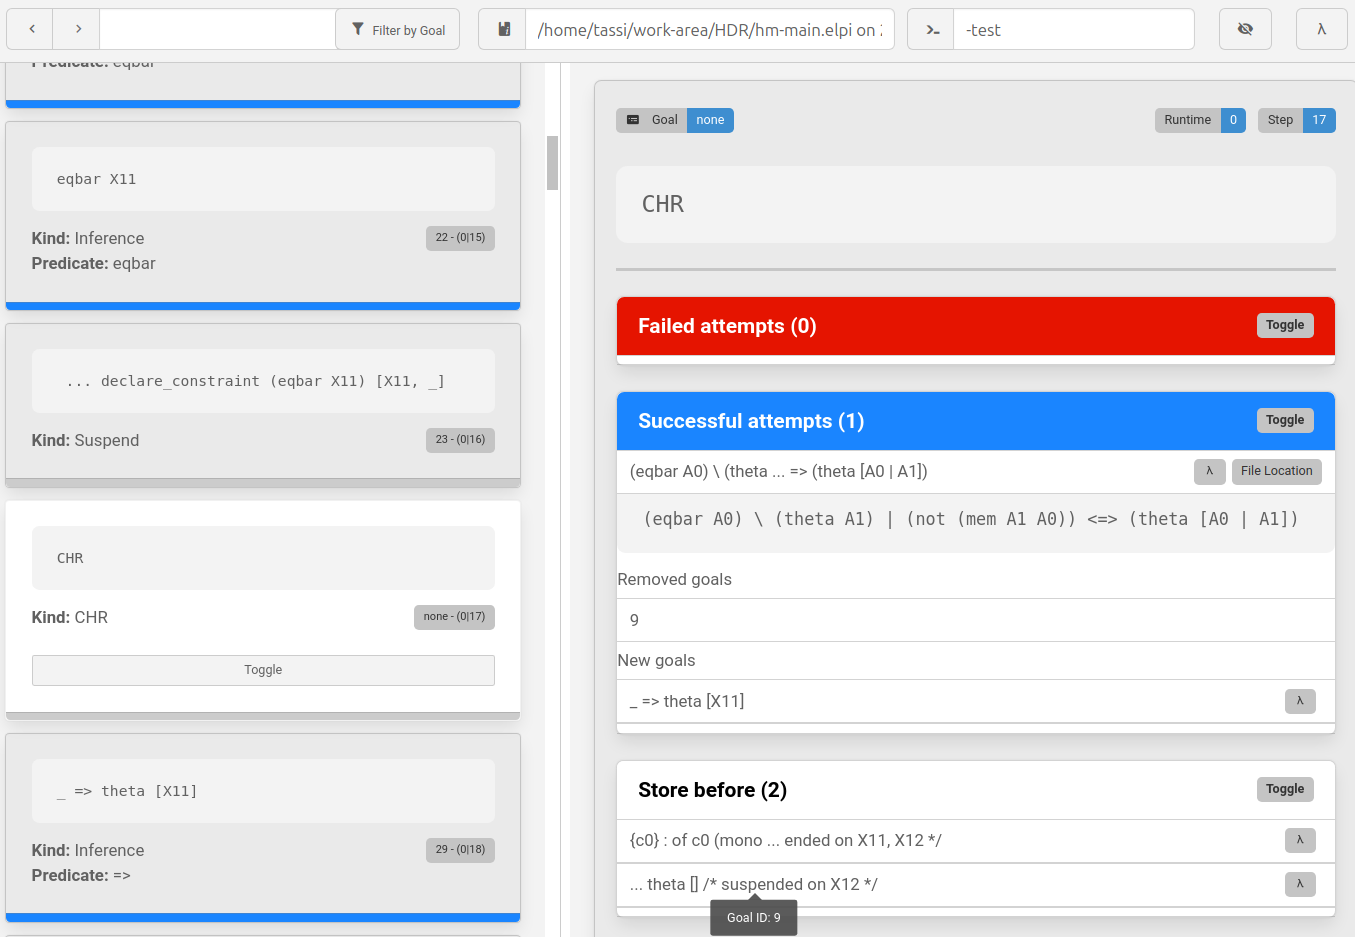
\includegraphics[width=.9\textwidth]{trace}
    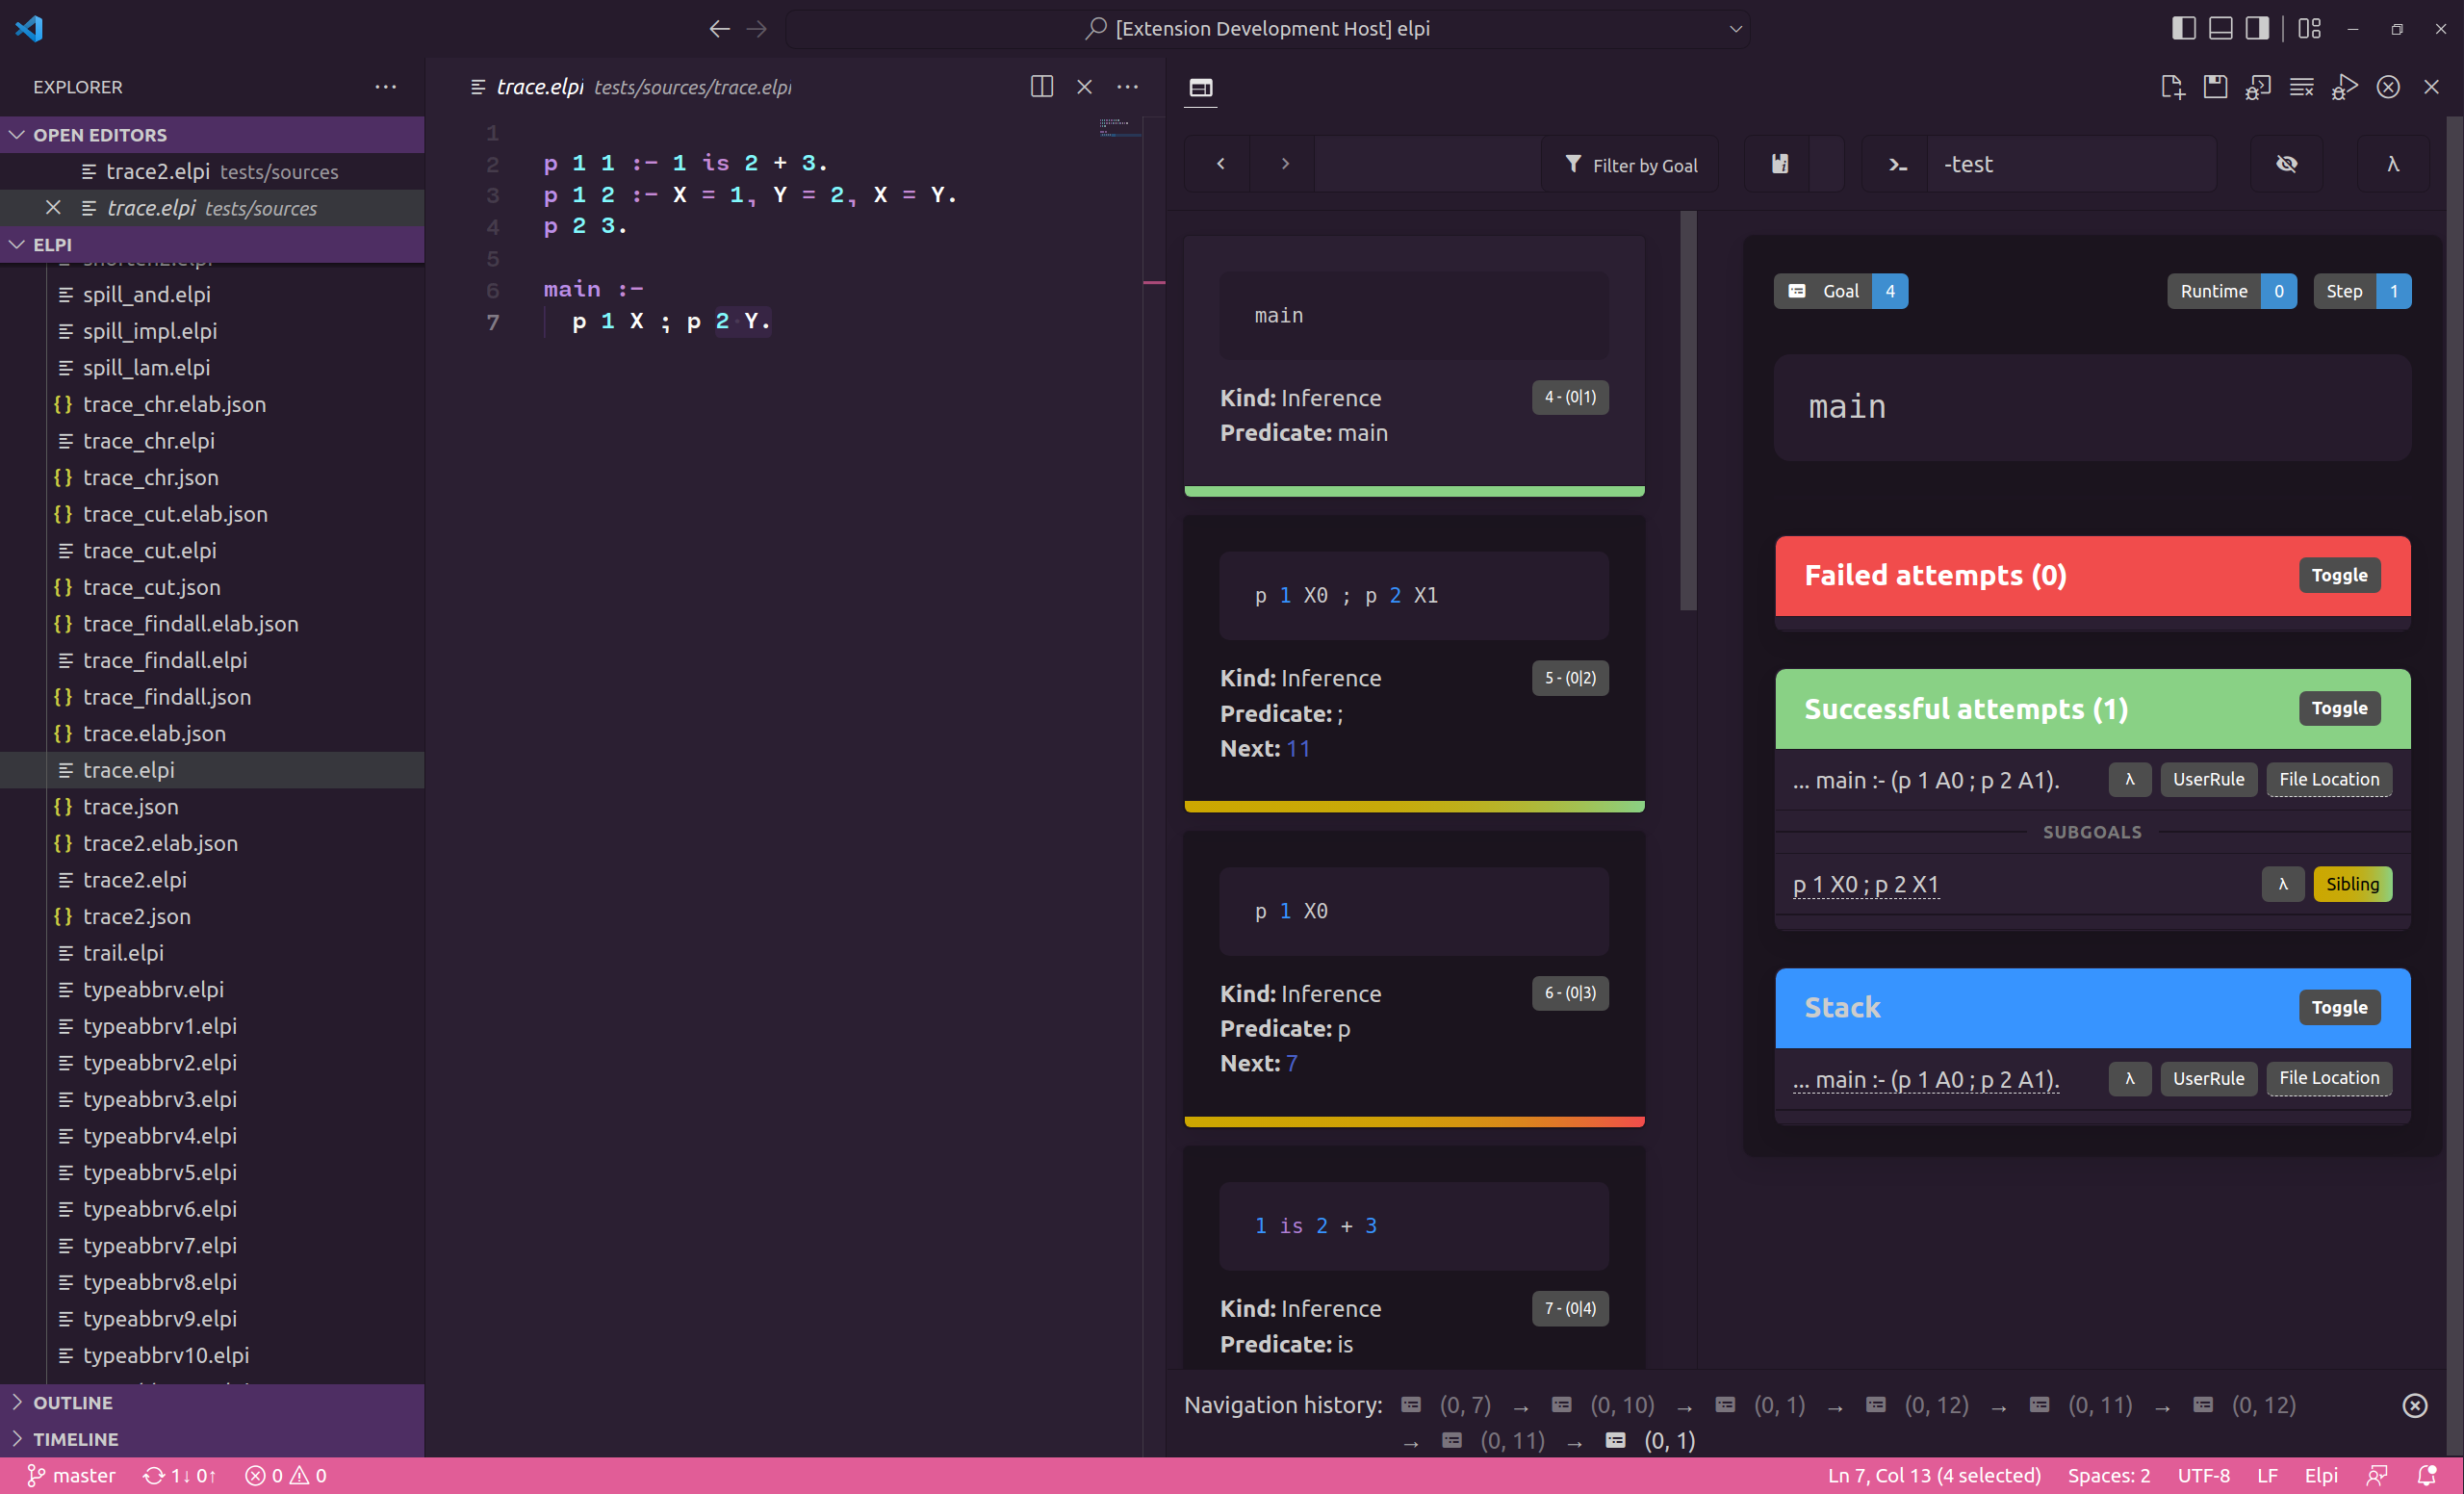
\includegraphics[width=.9\textwidth]{elpi-tracer}
    \caption{Trace browser\label{fig:trace}}
\end{sidewaysfigure}

Julien Wintz developed a trace browser (\cref{fig:trace}) based on web
technologies, making it easy to integrate into Visual Studio Code. It displays
the trace as a mailbox of events. Each event corresponds to the application of
a rule of the operational semantics~\cref{sec:sem}, and has pointers forward
to all subgoals and backward to the ancestor (via the stack). The trace is
also searchable.

The main limitation is that the implementation currently handles only
``small'' traces (below 20 megabytes), as it loads the trace upfront
and web apps are run in a memory constrained sandbox by VSCode.
Removing
this limitation is possible and planned.

\section{Benchmarks}

In~\cite{dunchev15lpar} we evaluate Elpi on a collection of synthetic
benchmarks and on a representative application. The synthetic tests are
grouped into three categories: first-order programs drawn from the Aquarius
test suite~\cite{aquarius} (crypto-multiplication, the $\mu$-puzzle, a
generalized eight-queens instance, and the Einstein zebra puzzle); higher-
order programs that lie inside the fragment \thefragment{} (see
\cref{fig:bench}); and a higher-order program outside the fragment, taken
from the Teyjus test suite for normalizing SKI-expressions.

Benchmarks within \thefragment{} include a type checker for $\lambda$-terms
(the \verb+of+ program discussed in~\cref{sec:hello}) and two evaluators that
compute expressions such as $5^5$ using Church numerals: one that follows
the call-by-value strategy and one the call-by-name one. The
type-checking benchmark is designed to measure the cost of traversing
binders: the test terms are largely projections and therefore contain many
\elpi{lam} nodes.

\begin{figure}
\begin{elpicode}
of (app M N) B :- of M (arr A B), of N A.
of (lam F) (arr A B) :- pi x\ of x A => of (F x) B.

copy (app M N) (app M2 N2) :- copy M M2, copy N N2.
copy (lam F) (lam F2) :- pi x\ copy x x => copy (F x) (F2 x).

cbv (lam F) (lam F2) :- pi x\ cbv x x => copy x x => cbv (F x) (F2 x).
cbv (app M N) R2 :- cbv N N2, cbv M M2, beta M2 N2 R2.

beta (lam F) T R2 :- !, subst F T R, cbv R R2.
beta H A (app H A).

subst F N B :- pi x\ copy x N => copy (F x) B.

cbn (lam F) (lam F2) :- pi x\ cbn x x => copy x x => cbn (F x) (F2 x).
cbn (app (lam F) N) M :- !, subst F N B, cbn B M.
cbn (app M N) R :- cbn M (lam F), !, cbn (app (lam F) N) R.
cbn (app X Y) (app X2 Y2) :- cbn X X2, cbn Y Y2.
\end{elpicode}
\caption{Source code of the second group of benchmarks\label{fig:bench}}
\end{figure}

\begin{center}
  \scriptsize 
  \begin{tabular}{|p{1.5cm}||c|r||c|r||c|c|}
    \hline
      \multicolumn{1}{|c||}{Test} &
      \multicolumn{2}{|c||}{Elpi} &
      \multicolumn{2}{|c||}{Teyjus} &
      \multicolumn{2}{|c|}{Elpi/Teyjus} \\
    \hline
    &  time (s)     & space (Kb)  & time (s) & space (Kb) &  time & space \\
    \hline
    \hline
    crypto-mult &  3.48 & 27,632  & 6.59 & 18,048 &  0.52 & 1.53 \\
    \hline    
    $\mu$-puzzle &  1.82 & 5,684 &  3.62 & 50,076 &  0.50 & 0.11 \\
    \hline
    queens &  1.41  & 108,324 &  2.02 & 69,968 &  0.69 & 1.54 \\
    \hline    
    zebra &  0.85 & 7,008 &  1.89 & 8,412 &  0.44 & 0.83 \\
    \hline     
    \hline
    of &  0.27 & 8,872 &  5.64 & 239,892 &  0.04 & 0.03 \\
    \hline
    cbv &  0.15 & 7,248 &  11.11 & 57,404  & 0.01 & 0.12 \\
    \hline
    cbn &  0.33 & 8,968 &  0.81 & 102,896  & 0.40 & 0.08 \\
    \hline
    %reduce\_cbv\_nocopy & ... & ... &  11.25 & 50,892  & ... & ... \\
    %\hline
    %reduce\_cbn\_nocopy & ... & ... &  0.52 & 70,760  & ... & ... \\
    %\hline
    \hline
    SKI &  1.32 & 15,472 &  2.68 & 8,896  & 0.49 & 2.73 \\
    \hline
    
  \end{tabular}
\end{center}

The results reported in the table show that Elpi performs particularly well
on programs inside \thefragment{} and remains competitive on the other
benchmarks. The variable behaviour of Teyjus on the reduction tests can be
explained by its explicit-substitutions machinery~\cite{NADATHUR200235} when
crossing binders. Explicit substitutions naturally suit a lazy strategy
such as call-by-name, although they incur some space overhead. By contrast,
explicit substitutions are detrimental in call-by-value: when the redex
argument is fully traversed the implementation tends to push suspended
substitutions to the term leaves, which defeats the goal of delaying
substitution. Forcing Teyjus to push explicit substitutions in the call-
by-name case reduces memory use but increases running time (about ten
seconds in our experiments), suggesting that the call-by-value timings are
dominated by the overhead of explicit substitutions.

Elpi avoids substitution when crossing binders; this design choice yields
both faster and more predictable behaviour. In the $5^5$ reduction test,
call-by-value outperforms call-by-name because it avoids duplicating
non-normal terms.

In~\cite{dunchev15lpar} we also compare Elpi and Teyjus on Helena, a type
checker for the formal system $\lambda\delta$~\cite{lambdadeltaJ1,lambdadeltaJ3a}.
Helena validates the proof terms of Landau's ``Grundlagen''~\cite{Jut79}
formalized in Automath. The reference Helena checker is implemented in
OCaml; our Elpi implementation follows its algorithm closely and falls
within \thefragment{}. The Elpi implementation is, however, substantially
shorter than the equivalent OCaml program: it is expressed in roughly fifty
rules.

Grundlagen is a corpus of 6911 items (about 8MB). When the benchmarks were
run (around 2015), Teyjus appeared to be limited by a fixed heap size of
256MB, which restricted it to verifying the first 2615 items. The tables
below report pre-processing time (Pre), which includes parsing and
compilation/elaboration, and verification time (Ver). We compare Elpi with
Helena, Teyjus, and Rocq. Rocq implements a type checker for a
$\lambda$-calculus that is strictly more expressive than $\lambda\delta$;
thus Rocq can type-check the proof terms directly but possibly with additional
overhead. We use Rocq timings as a reference for the order of magnitude when
comparing Elpi against a state-of-the-art interactive prover. Where
applicable we contrast native and interpreted executions.
\begin{center}
  \scriptsize 
\begin{tabular}{|l|c|c|c|}
\hline
\multicolumn{4}{|c|}{Time (s) for 2615 items only}\\
\hline
 & Elpi          & Teyjus  & Elpi/Teyjus        \\
\hline
Pre      & 2.55 & 49.57 & 0.05 \\
\hline
Ver      & 3.06 & 203.36 & 0.02 \\ \hline
RAM (Mb) & 91,628 & 1,072,092 & 0.09 \\
\hline
\end{tabular}
~~
\begin{tabular}{|l|c|c|c|c|c|}
\hline
\multicolumn{6}{|c|}{Time (s) for all 6911 items}\\
\hline
Task                   &\multicolumn{2}{|c|}{Helena}         & Elpi          & \multicolumn{2}{|c|}{Rocq 8.3}            \\
                 &interp. & comp.& interp. &interp. & comp.\\ \hline
Pre & 2.42 & 0.41 & 9.04 & 49.28 & 8.83 \\
\hline
Ver & 4.40 & 0.33 & 13.90 & 7.21 & 1.19\\ % coqchk.opt: 3.90
\hline
\end{tabular}
\end{center}

The data indicate that Elpi behaves similarly to Teyjus on first-order
programs. The observed advantage of Elpi is likely attributable to the more
efficient garbage collector available in OCaml. The same behaviour is seen
for higher-order programs that lie outside \thefragment{}.

Within \thefragment{} Elpi is noticeably more efficient. Teyjus only
matches Elpi when the program benefits from a lazy treatment of
substitutions; even in that case Teyjus incurs a substantial memory
overhead.

Because Elpi is designed to serve as an extension language for Rocq, the
most relevant comparison is with Rocq's native OCaml implementation. Elpi
is roughly an order of magnitude slower than Rocq, which is expected for an
interpreter; we consider this penalty acceptable in light of the benefits of
rapid prototyping and extensibility. Moreover, Elpi programs can invoke
efficient Rocq routines when necessary. In short, Elpi aims to provide a
high-level language for manipulating syntax trees while remaining fast
enough for practical use.


\chapter{Rocq-Elpi}\label{sec:rocq}


While Elpi is a standalone language and software project, it was designed to
serve as an \emph{extension language} for Rocq~\cite{Coq-refman}.
The glue between Elpi and Rocq is called Rocq-Elpi.

My definition of this role, \emph{extension language}, is largely influenced by
the Lua programming language~\cite{10.5555/1200583}. Lua is an extension
language for applications written in C and is widely used in the open source
world and the gaming industry. Its purpose is to provide an easy way to extend
the host application. Lua is easy to host because its FFI is well curated;
exposing the internals of the application to the extension language requires
limited effort from the application developer. It is easier to program in Lua
than in C, because Lua is a higher-level language: for example, it features
automatic memory management and provides dictionaries as a built-in data
structure. Finally, it is easy for a user to get started with Lua because no
special development environment is needed -- the host application is sufficient,
since Lua is an interpreter.
Elpi aims to do the same for OCaml~\cite{leroy3ocaml}, with Rocq as the
host application of
interest.

In academia, the same role is often called a meta-programming framework. Rocq's
main data type, terms, are programs, and Elpi programs manipulate Rocq
programs. In this sense, Elpi programs operate at the meta level.


\section{Why extending Rocq in OCaml is hard}

Fortunately, OCaml features automatic memory management, types, and algebraic
data. It is much, much higher level than C. So why is it hard to extend Rocq?
Why do we need another language?

\index[concepts]{Gallina}
The first difficulty is that the complexity of Rocq's core language,
\emph{Gallina}, is not completely hidden by the algebraic data types
provided by the OCaml
programming language. The missing features are encoded, and it is hard to
completely hide them from the programmer via curated APIs. In particular,
Gallina terms feature binders and holes.

Binders pose two problems of their own and interact poorly with holes. The
first problem is that they are typically encoded with numbers (De Bruijn
indexes), and it is all too easy to forget to shift a term. The second
problem is that when a binder is crossed, one must always remember something
about it, typically the type of the bound variable. Hence, programs have to
pass around typing contexts (aka environments). It is tempting not to do this
upfront, but expecting all developers -- especially casual ones -- to be disciplined
seems a lost battle. We deeply agree with Mc Bride on this~\cite[page 20]{mcbride}:
``Mantra: $\Gamma$ is with me, wherever I go.''

Holes are missing subterms and come with metadata: a typing sequent. Since the
same hole can have multiple occurrences, a single sequent is stored on the side of
terms. Moreover, since binders may be reduced away, each occurrence has an
explicit substitution. So there is a state that that is associated with the terms --
a state to be threaded in a functional setting. This state also gathers universe
constraints, as required by Rocq's typical ambiguity (writing \rocq{Type} with
no explicit level).
Assignments are also part of this state, and the bugs that stem from the
programmer forgetting it even gave rise to odd concepts among Rocq developers
like ``evar sensitive'' (evar is the name for holes). If one forgets to look at
terms through the right assignment (e.g., uses the empty one), the behavior is
hard to debug: it is like OCaml code that behaves differently depending on
whether a reference \ocaml{x} was originally given the value 42, or if it was
later updated to that value.
The example is not an exaggeration: the state accompanying holes is really like
a heap, and if one has to manage it by hand, it is like going back to manual
memory management, pointer dereferencing (with no types), and no garbage
collection. It does not sound that different from C.

The second difficulty is not inherent in OCaml, but rather an artifact of the
history of Rocq. The APIs are not well curated. Exposing some of them to the
extension language is a very good opportunity to incrementally produce a
coherent set of APIs.

Finally, there is the challenge of setting up the development environment and
process. Even when a user is past the inevitable frustration of setting up the
right compiler and tools, an embedded interpreter still offers some
advantages -- especially if the language is rule-based. One can iterate faster,
without even restarting the host application, and sometimes even modify the
code at a distance: if the code is defined far away, in a library being used,
one can replace bits of its code by replacing a rule defined there with a
new one defined here, where the problem shows up, and in the end conduct a
much faster investigation.

\section{Encoding Rocq terms and contexts}\label{GALLINA}


The main data type that Rocq-Elpi programs work with is the one of Rocq terms. The
first aspect of terms worth describing is the pointers to global objects.
While \elpi{constant}, \elpi{inductive}, and \elpi{constructor} are opaque
data (as in \cref{sec:opaquedata}), their nature is exposed as an algebraic
data type.

\begin{elpicode}
kind gref type.
type const constant -> gref.            % Nat.add, List.append, ...
type indt  inductive -> gref.           % nat, list, ...
type indc  constructor -> gref.         % O, S, nil, cons, ...
\end{elpicode}

\noindent
In the examples part of this document we shall use the string notation for
these three opaque data types, althought in real code one needs to resolve
a \elpi{string} to a \elpi{gref} via the \elpi{rocq.locate} API.

Global objects are injected into the term data type via the \elpi{global} term
constructor and its variant \elpi{pglobal}, which is dedicated to
universe-polymorphic global objects.

\begin{elpicode}
kind term type.
type global  gref -> term.
type pglobal gref -> univ-instance -> term.
type sort    sort -> term.                 % Prop, Type@{i}, SProp
\end{elpicode}

\noindent
We omit the code for the \elpi{sort} data type and just remind it
represents Rocq sorts such as \rocq{Prop} and \rocq{Type}.

Instead we focus on the three
binders: \elpi{fun} and \elpi{prod} for abstraction, and \elpi{let} for
abbreviation. In addition to the higher-order argument, the detail common to
all of them is the \elpi{name} argument. It stands for pretty-printing
information, e.g., the bound variable name as written by the user. It is important
to note that \elpi{name} is an opaque data type with a trivial equality test.
That is, the names ``x'' and ``y'' are equal in Elpi, although they hold
different values in OCaml. This is key to aligning the equational theory of
the meta-language Elpi with a sensible notion of equality for the object
language Gallina, namely $\alpha$-equivalence.

\begin{elpicode}
type fun  name -> term -> (term -> term) -> term.            % λ
type prod name -> term -> (term -> term) -> term.            % ∀
type let  name -> term -> term -> (term -> term) -> term.    % let
\end{elpicode}

\noindent
Application is n-ary, with the head and arguments held in a list. This choice,
over binary application as in~\cref{sec:hello}, eases access to the head:
according to our experience, the vast majority of rules are discriminated by
the head constant of the terms they operate on.
\begin{elpicode}
type app       list term -> term.                     
\end{elpicode}
\noindent
The Rocq pattern matching constructor packs together the scrutinee, a term
used to uniformly assign a type to branches, and a list of branches.
\begin{elpicode}
type match     term -> term -> list term -> term.   
\end{elpicode}
\noindent
The
fixpoint operator is a binder for the recursive call and carries the index of
the decreasing argument. 
\begin{elpicode}
type fix       name -> int -> term -> (term -> term) -> term.
\end{elpicode}
\noindent
Finally, a single constructor holds all primitive
values, e.g., 63-bit integers, floating point numbers, and primitive record
projections.
\begin{elpicode}
type primitive primitive-value -> term.
\end{elpicode}
What is worth focusing on is the representation of contexts since it
defines a convention to be used when crossing binders. In turn
this convention enables APIs to be called deep inside terms. Two
context entries need to be available: one for abstraction and one for
abbreviation.

\begin{elpicode}
pred decl i:term, o:name, o:term.                 % Var Name Ty
pred def  i:term, o:name, o:term, o:term.         % Var Name Ty Bo
\end{elpicode}

The first argument of each is, by convention, a bound variable, and is
expected to be passed as input in order to retrieve the associated pretty
printing information, the type, and, in the case of abbreviation, the body. In
light of this, code that crosses a binder is expected to declare either a
\elpi{decl} or a \elpi{def} hypothetical rule for the bound variable as
follows:
\begin{elpicode}
some-pred (fun N T F) :-
  pi x\ decl x N T => some-pred (F x).
\end{elpicode}
\noindent
And convenience macros help the programmer obey the discipline. Note how
the macro arguments are the same of the term constructor it crosses:
\begin{elpicode}
some-pred (fun N T F) :-
  @pi-decl N T x\ some-pred (F x).
\end{elpicode}
\noindent
As a result of this convention, one can call \elpi{rocq.typecheck} deep inside
a term. As described in~\cref{sec:API}, a built-in predicate can be equipped with a
\ocaml{ctx_readback} function, such as \ocaml{proof_context} in the code
below. The \ocaml{term} contextual conversion can thus access a Rocq context
when operating its readback or embedding code.

\begin{ocamlcode}
MLCode(Pred("rocq.typecheck",
  CIn(term, "T",
  CInOut(B.ioargC term, "Ty",
  InOut(B.ioarg B.diagnostic, "Diagnostic",
  Full (proof_context, "typchecks a term T ...")))),
    (fun t ety diag _ proof_context _ state ->
      let sigma = get_sigma state in
      let sigma, ty = Typing.type_of proof_context.env sigma t in
      let state, assignments = set_sigma ~depth state sigma in
      ...
\end{ocamlcode}


Here, the \ocaml{t} and \ocaml{ety} values are read back in the
\ocaml{proof_context.env} Rocq context, which is also passed to the type
checker to synthesize the type of \ocaml{t}, and later (in the omitted code)
to unify the inferred type with the expected one \ocaml{ety}, when provided.
The \ocaml{B.diagnostic} datum is either the Elpi value \elpi{ok} or
\elpi{error "message"}; thus, a call \elpi{rocq.typecheck T Ty ok} is the
idiom to assert that \elpi{T} is well-typed of type \elpi{Ty}.
~\\

The only missing piece is \ocaml{sigma}, the environment assigning type
judgements to holes, i.e., the call to the \ocaml{get_sigma} and
\ocaml{set_sigma} APIs, which we focus on in the next section.

\section{Encoding holes}\label{sec:hoasholes}


Each Rocq hole has an entry in \ocaml{sigma} that resembles a sequent.
We show in~\cref{fig:sigma} simplified code from the sources of Rocq 9.0.

\begin{figure}[h]
\begin{ocamlcode}
module Evar : sig

  type t = int                             (* hole handle    *)
  module Map : Map.s with type key = t     (* map on holes   *)
  ...

module Evd : sig

  type evar_body =
    | Evar_empty                      (* no inhabitant yet   *)
    | Evar_defined of constr          (* proof term          *)

  type evar_info = {
    evar_concl : constr;              (* sequent conclusion  *)
    evar_hyps  : named_context_val;   (* sequent context     *)
    evar_body  : evar_body;           (* optional proof term *)
    ...
  }

  type evar_map = {
    (* Evars, split in two for performance reasons *)
    defn_evars : evar_info Evar.Map.t;
    undf_evars : evar_info Evar.Map.t;

    (* Universe constraints *)
    universes  : UState.t;
    ...
  }
\end{ocamlcode}
\caption{Rocq's evar map\label{fig:sigma}}
\end{figure}

In Elpi, we represent this data -- referred to as \ocaml{sigma} -- as a set of
\elpi{evar} constraints. Such a constraint links a \emph{raw} Elpi unification
variable \elpi{RawEv}, a type, and the \emph{elaborated} Elpi unification variable
\elpi{Ev} (their meaning is clarified below).
The constraint should live in a context of hypothetical rules \elpi{Ctx}
assigning types to bound variables. In other words, each evar is represented
by the result of suspending a query as follows:

\begin{elpicode}
  pi x1\ .. pi xn\ Ctx =>
    evar RawEv Ty Ev
\end{elpicode}

\noindent in a program with the following suspension rules:

\begin{elpicode}
pred evar i:term, i:term, o:term. % RawEv Ty Ev
evar X Ty R :- var X, var R,      !,
  declare_constraint (evar X Ty R) [X, R].
evar X Ty R :- var X, not(var R), !,
  rocq.typecheck R Ty ok, X = R.
evar X Ty R :- not(var X), var R, !,
  rocq.elaborate-skeleton X Ty R ok.
\end{elpicode}

\noindent
The code above enforces the following invariants:

\begin{itemize}
  \item each unassigned Rocq evar has a corresponding Elpi constraint
  \item \elpi{Ev} can be assigned to a term \elpi{R} only if
        \elpi{R} has type \elpi{Ty} in context \elpi{Ctx}
  \item \elpi{RawEv} can only be assigned to a term \elpi{X} if
        \elpi{X} elaborates to a term \elpi{R} such that
        the previous condition holds
\end{itemize}

\noindent
In the code above, \elpi{rocq.elaborate-skeleton} is an API very similar to
\elpi{rocq.typecheck}, but that does not modify its input in place. Instead, it
uses its input as a skeleton term that is copied. This allows for changes to
the structure of the term, such as inserting explicit coercions to implement
type casts. The API corresponds to the code that Rocq runs on any input term
written by the user, while \elpi{rocq.typecheck} corresponds to code
internally used by Rocq tactics to build well-typed terms.

In order to declare a new \elpi{evar} constraint at any time, even if the
current $\lambda$Prolog program has more names and hypothetical rules than
needed, we use the following predicate:

\begin{elpicode}
pred declare-evar i:list prop, i:term, i:term, i:term.
declare-evar Ctx RawEv Ty Ev :-
  declare_constraint (declare-evar Ctx RawEv Ty Ev) [_].

constraint declare-evar evar def decl {
  rule \ (declare-evar Ctx RawEv Ty Ev) <=> (Ctx => evar RawEv Ty Ev).
}
\end{elpicode}

\noindent
Note how \elpi{declare-evar} uses a CHR rule to craft a new goal with a
precise context \elpi{Ctx}, regardless of the context under which
\elpi{declare-evar} is run. Indeed, a Rocq API that is called deep
inside a term and encounters a new hole will add an entry for it to Rocq's
evar map, but also generate a \elpi{declare-evar}, and hence an \elpi{evar}
constraint in Elpi. This is possible thanks to the type of contextual
conversions (\cref{sec:hodata}), which includes a list of extra goals to be generated in response
to the conversion.

The only missing pieces are the \ocaml{get_sigma} and \ocaml{set_sigma}
APIs. Their role is to synchronize updates to \ocaml{sigma} in both
directions. The former, \ocaml{get_sigma}, is the simplest, since a Rocq
datum of type \ocaml{evar_map} is stored in the extensible state of Elpi.

To implement the other, we take advantage of an API offered by Elpi: a
bidirectional map linking Rocq unification variables and Elpi holes.

\begin{ocamlcode}
module FlexibleData : sig
  module Elpi : sig type t ... end
  module type Host = sig type t ... end
  module Map : functor(Host : Host) -> sig
    type t
    val empty : t
    val add   : Elpi.t -> Host.t -> t -> t
    val elpi  : Host.t -> t -> Elpi.t
    val host  : Elpi.t -> t -> Host.t
    val fold  :
      (Host.t -> Elpi.t -> term option -> 'a -> 'a) -> t -> 'a -> 'a
\end{ocamlcode}

\noindent
The extensible state contains two instances of the bidirectional map
described above: one for raw holes and one for elaborated holes. A Rocq
\ocaml{Evar.t} is linked to one of each.
To propagate changes to \ocaml{sigma} performed by Rocq, we fold
over the set of linked evars to check if they have been assigned. If so, we
remove the corresponding \elpi{evar} constraint and generate the corresponding
assignment as an Elpi unification problem between the hole and the Rocq term.

%%%%%%%%%%%%%%%%%%%%%%%%%%%%%%%%%%%%%%%%%%%%%%%%%%%%%%%%%%%%%%%%%%%%%%%%%%%%%%%
%%%%%%%%%%%%%%%%%%%%%%%%%%%%%%%%%%%%%%%%%%%%%%%%%%%%%%%%%%%%%%%%%%%%%%%%%%%%%%%
%%%%%%%%%%%%%%%%%%%%%%%%%%%%%%%%%%%%%%%%%%%%%%%%%%%%%%%%%%%%%%%%%%%%%%%%%%%%%%


\section{Vernacular language integration}


The vernacular language of Rocq allows one to organize formalized knowledge,
in particular to give names to Gallina terms and attach metadata to them.
Rocq-Elpi extends the vernacular language with a few commands to declare, run,
and modify Elpi programs.

For convenience, programs are divided into commands and tactics. Both run Elpi
code, but the entry point is different; moreover, tactics can only be executed
in Rocq proof mode.

\subsection{Commands}

A command is declared with \rocq{Elpi Command} followed by a name. Initially,
a command only contains the glue code for Rocq, such as the HOAS data type of
terms and the built-in predicates. Extra code can be added to a command via
\rocq{Elpi Accumulate}. Accumulated code can be either static (e.g., from a
file or a string) or dynamic (from a database; see~\cref{sec:homo}).

A command \texttt{hello} is executed with \rocq{Elpi hello} followed by
arguments. The entry point is the \elpi{main} predicate
that receives a list of arguments. The \elpi{argument} data type has constructors for built-in data
types such as strings or numbers, as well as Gallina terms.

\begin{rocqcode}
Elpi Command hello.
Elpi Accumulate hello lp:{{
  main [str X] :- rocq.say "Hello" X.
}}.
Elpi hello "reader".    (* prints "Hello reader" *)
Fail Elpi hello 46.     (* fails *)
\end{rocqcode}

The simple program above calls the \elpi{rocq.say} built-in whenever the
command is passed a string. Since the entry point \elpi{main} has no rule for
arguments of the form \elpi{int X}, the second calls fails.

Interested readers can consult the comprehensive tutorial on Elpi commands
~\cite{tuto:commands}, which is part of the Rocq-Elpi software distribution.

\subsection{Tactics}


Tactics are built in a similar way, with the main difference being that the
entry point is called \elpi{solve}, which receives as arguments not only the
arguments passed to the tactic, but also the goal on which the tactic
operates.

\begin{rocqcode}
Elpi Tactic intro.
Elpi Accumulate intro lp:{{
  solve (goal _ _ _ _ [str ID] as G) GS :- !,
    std.assert! (rocq.ltac.id-free? ID G) "name already taken",
    rocq.id->name ID N,
    refine (fun N _ _) G GS.
}}.
Goal ∀P, P -> P /\ P.
elpi intro "p".
Fail elpi intro "p". (* Error: name already taken *)
elpi intro "Hp".
\end{rocqcode}


In the example above, the tactic expects to receive a string \elpi{ID}; it
checks that no Rocq proof variable is already using the name \elpi{ID}, and finally
refines\footnote{The \elpi{refine} API is akin to Rocq's \rocq{refine}
tactic: it makes progress on one goal by
providing a term containing holes, holes for which new goals are generated}
the goal with a lambda abstraction, which is the proof term for the
logical rule of introduction of universal quantification or implication.
Note that the check for the name being free is just for convenience: a
collision would not result in name capture in Elpi, and when translated back
to Rocq, the deepest variable would be forcibly renamed to avoid capture in Rocq too.

Interested readers can consult a longer tutorial on Elpi tactics
~\cite{tuto:tactics}, as well as look into eltac~\cite{app:eltac},
a collection of basic Rocq tactics rewritten in Elpi for didactic purposes.

\subsection{Databases}\label{sec:homo}


A database is, in essence, an Elpi program, but unlike commands and tactics,
it cannot be executed directly. It constitutes a piece of code that is
accumulated into commands or tactics \emph{by name}. This means that whenever
a program runs, it sees the current contents of the databases it accumulates,
not their contents at the time the command was initially declared.


A typical database consists of a single predicate, possibly with some default
rules. The \rocq{Elpi Db} command declares a database.

\begin{rocqcode}
Elpi Db age.db lp:{{
  pred age o:string, o:int.

  % the Db is empty for now, we put a rule giving a
  % descriptive error and we name that rule "age.fail".
  :name "age.fail"
  age Name _ :- rocq.error "I don't know who" Name "is!".
}}.
\end{rocqcode}


Elpi rules can be assigned a name via the \texttt{:name} attribute. Named rules
serve as anchor points for new rules when they are added to the database.


A command to print the age of a given name can be declared as follows:

\begin{rocqcode}
Elpi Command age.
Elpi Accumulate Db age.db.
Elpi Accumulate lp:{{

  main [str Name] :-
    age Name A,
    rocq.say Name "is" A "years old".

}}.

Fail Elpi age bob. (* I don't know who bob is! *)
\end{rocqcode}


We can add entries to the database manually as follows:

\begin{rocqcode}
Elpi Accumulate age.db lp:{{

  :before "age.fail"     % we place this rule before the catch all
  age "bob" 24.

}}.

Elpi age bob. (* bob is 24 years old *)
\end{rocqcode}


We do not expect users of Rocq commands written in Elpi to know the syntax of
Elpi, nor the commands to manipulate its programs, and even less to actually
know that the Rocq commands they run are implemented in Elpi.


For this reason, Rocq-Elpi provides APIs to extend databases from Elpi. Here,
we craft a new command \rocq{set_age} that uses this API.

\begin{rocqcode}
Elpi Command set_age.
Elpi Accumulate Db age.db.
Elpi Accumulate lp:{{

  main [str Name, int Age] :-
    TheNewRule = age Name Age,
    rocq.elpi.accumulate _ "age.db"
      (clause _ (before "age.fail") TheNewRule).

}}.

Elpi set_age "alice" 21.
Elpi age "alice". (* alice is 21 years old *)
Elpi set_age "mallory" 24.
Elpi age "mallory". (* mallory is 24 years old *)
\end{rocqcode}


The same databases can be accumulated by commands and tactics in order to
share a state -- a common knowledge base that typically grows as the commands
or tactics are used in a Rocq library.

\subsubsection{Homoiconicity and rules}


There are two characteristics of Elpi that make databases both possible and
convenient to use.


The first is that Elpi is a homoiconic language: it can manipulate its own
syntax. The following line illustrates this property:
\begin{elpicode}
% build code
TheNewRule = age Name Age,
\end{elpicode}
This is the simplest evidence of it: \elpi{TheNewRule} contains a piece of
Elpi code built from the \elpi{age} predicate and the two arguments passed to
\elpi{main}. Since construction and inspection are conflated into unification
in logic programming, the same line can be used to analyze the syntax of a
piece of code in order to extract the name and age. Moreover, since expressions
and commands are not confused in logic programming, there is no confusion
in the user's intention: she wants to build/inspect a piece of code, not to run
it.\footnote{In other words the quotation operator \texttt{'} of the Lisp family
of languages is not needed.}


The second helpful characteristic of Elpi is that code is organized into rules,
meaning that \elpi{age Name Age} is an entire code unit that one can build,
inspect and run. In comparison, the OCaml code for the \ocaml{age} function is a
single expression (a single unit):

\begin{ocamlcode}
let age s =
  match s with
  | ("bob" | "mallory") => 24
  | "alice" => 21
  | _ => failwith ("I don't know who " ^ s ^ " is!")
\end{ocamlcode}


While it is certainly possible to traverse the syntax tree above and add a
pattern match branch before the last one, such manipulation is not entirely
trivial. To make it so, one should opt out of most syntactic sugar and commit
to using a syntactic form that is as close as possible to that of a rule-based
language:
\begin{itemize}
  \item making all variable bindings local to the pattern matching branch
  \item making all rules syntactically independent
\end{itemize}


The code below respects these points. Note that the \ocaml{s} binding is now
local to the last branch, and there is a clear separation between the bob and
mallory branches:

\begin{ocamlcode}
let age = function
  | "bob" => 24
  | "alice" => 21
  | "mallory" => 24
  | s => failwith ("I don't know who " ^ s ^ " is!")
\end{ocamlcode}
  
~\\
The syntactic price one pays when writing Elpi code is thus partially
compensated by the ease of extending existing code. The example in the
following section makes good use of this possibility.

\section{Example: proof transfer}\label{sec:tb}


As a simple example, we present a tactic and a command that communicate via a
database. The tactic \rocq{to_bool} transfers a goal from the realm of
propositions to that of computable (boolean) tests (i.e., effectively decidable
propositions). The command \rocq{register_decision} takes a proof of
equivalence between a proposition and a boolean test and compiles it into an
Elpi rule. The database contains all known rules for translating propositions
into tests: it is queried by \rocq{to_bool} and populated by
\rocq{register_decision}.


It is customary to organize Rocq-Elpi code in this way. The key advantage is that
\rocq{to_bool} is extensible: when a new Rocq predicate is declared and a new
corresponding test is defined, it is sufficient to call
\rocq{register_decision} to extend \rocq{to_bool}.



We assume a Rocq environment with the following lemmas. The \rocq{reflect}
predicate~\cite{assia_mahboubi_2022_7118596} links a proposition with a boolean test: \rocq{reflect P b} means
\rocq{P} holds if and only if \rocq{b = true}.

\begin{rocqcode}
Lemma evenP n : reflect (is_even n) (even n).

Lemma andP  {P Q : Prop} {p q : bool} :
  reflect P p -> reflect Q q -> reflect (P /\ Q) (p && q).

Lemma elimT {P b} :
  reflect P b -> b = true -> P.
\end{rocqcode}



The database holds rules for the \elpi{tb} predicate. For simplicity, we only
deal with one direction of the equivalence: we relate a proposition with its
equivalence proof (disregarding the associated boolean test).

\begin{rocqcode}
Elpi Db tb.db lp:{{

% [tb P R] finds [R : reflect P b] for some b
pred tb i:term, o:term.

:name "tb:fail"
tb Ty _ :- rocq.error "Cannot solve" {rocq.term->string Ty}.

}}.
\end{rocqcode}


Initially, the database contains only one rule, which aborts the search with
an error message. All additional rules must be placed before this one.


The \rocq{to_bool} tactic is built as follows, on top of the database.

\begin{rocqcode}
Elpi Tactic to_bool.
Elpi Accumulate Db tb.db.
Elpi Accumulate lp:{{

solve (goal Ctx _ Ty _ [] as G) [G1] :-
  tb Ty P,
  refine {{ elimT lp:P _ }} G [G1].

}}.
\end{rocqcode}


The tactic simply queries the database for a proof \elpi{P} that the goal is
related to a boolean test \rocq{b}, then refines the goal.
with \rocq{elimT lp:P _}. The hole stands for the proof
of \rocq{b = true}, i.e., the subgoal \elpi{G1}.


The most interesting part of this example is how the database is populated.
We shall write a \elpi{compile} procedure that, given \rocq{evenP} and
\rocq{andP}, synthesizes the following Elpi code:

\begin{elpicode}
tb {{ is_even lp:N }} {{ evenP lp:N }} :- !.
tb {{ lp:P /\ lp:Q }} {{ andP lp:PP lp:QQ }} :- !, tb P PP, tb Q QQ.
\end{elpicode}


As sketched in~\cref{sec:homo}, the two rules above correspond to the
following (closed) Elpi terms:

\begin{elpicode}
pi N\ tb {{ is_even lp:N }} {{ evenP lp:N }} :- [!]
pi P Q PP QQ\ tb {{ lp:P /\ lp:Q }} {{ andP lp:PP lp:QQ }} :-
  [!, tb P PP, tb Q QQ].
\end{elpicode}


It is worth unfolding quotations to see that a few more quantifications are
necessary for the second rule:

\begin{elpicode}
pi P Q p q PP QQ\
  tb (app[global (indt "and"), P, Q])
     (app[global (con "andP"), P, Q, p, q, PP, QQ]) :-
  [!, tb P PP, tb Q QQ].
\end{elpicode}
  


Now that all quantifications are explicit, we can look at the types of
\rocq{evenP} and \rocq{andP} and observe how each \elpi{pi} Elpi
quantification corresponds to a Rocq quantification (dependent or not), and
how Rocq premises correspond to recursive calls in Elpi.

\begin{rocqcode}
evenP : ∀n, reflect (is_even n) (even N).
andP : ∀P Q p q,
  reflect P p -> reflect Q q -> reflect (P /\ Q) (p && q).
\end{rocqcode}

We are now set to write our little rule compiler.
The \elpi{compile} predicate has three inputs and one output. The first input
is the type of a lemma, and the second is the proof of that lemma; the
relation between the first two arguments is a key invariant. The third
argument is a list of recursive calls, while the output is the code of the
Elpi rule being generated.

\begin{elpicode}
pred compile i:term, i:term, i:list prop, o:prop.

compile {{ reflect lp:Ty _ }} P Hyps (tb Ty P :- [! | Hyps]).

compile {{ reflect lp:S _ -> lp:T }} P Hyps (pi h\ C h) :- !,
  pi h\ compile T {{ lp:P lp:h }} [tb S h | Hyps] (C h).

compile {{ ∀x, lp:(T x) }} P Hyps (pi h\ C h) :-
  pi x\ compile (T x) {{ lp:P lp:x }} Hyps (C x).
\end{elpicode}


The first rule is the base case. When we reach the conclusion of the lemma
\rocq{reflect lp:Ty _}, we know that the second argument \elpi{P} is a proof
of that fact; hence, \elpi{tb Ty P} is a correct head for the rule. The
premises of the rule are the \elpi{Hyps} recursive calls, prefixed with a cut.


The second rule handles premises that are turned into recursive calls. In this
case, the rule being synthesized features an extra \elpi{pi} quantification,
and the \elpi{Hyps} list grows longer.
The \elpi{h} variable stands for the proof
obtained by the recursive call -- a proof of \rocq{reflect lp:S _} -- hence
a value we can pass to \elpi{P} obtaining the Rocq term
\rocq{lp:P lp:h} that is a proof of \elpi{T}.


The last rule is a simpler version of the second; in this case, the
quantification is not a premise. In this case we do not extend \elpi{Hyps}.


The code of the \rocq{register_decision} command locates the given lemma,
finds its type, and generates the new rule \elpi{C}. Finally, it adds the rule
to the database before the \elpi{"tb:fail"} anchor point.

\begin{rocqcode}
Elpi Command register_decision.
Elpi Accumulate Db tb.db.
Elpi Accumulate lp:{{
    
main [str S] :-
  rocq.locate S GR,
  rocq.env.typeof GR Ty,
  compile Ty (global GR) [] C,
  rocq.elpi.accumulate _ "tb.db" (clause _ (before "tb:fail") C).

}}.
\end{rocqcode}


We can now populate the database and test our tactic.

\begin{rocqcode}
Elpi register_decision andP.

Lemma test : is_even 6 /\ is_even 4.
Proof.
elpi to_bool. (* Error: Cannot solve is_even 6 *)
Abort.

Elpi register_decision evenP.

Lemma test : is_even 6 /\ is_even 4.
Proof.
elpi to_bool. (* even 6 && even 4 = true *)
simpl.        (* true = true *)
trivial.
Qed.
\end{rocqcode}
  

The Rocq snippet calls the \rocq{to_bool} tactic in a scenario where a
predicate is not (yet) registered, resulting in an explanatory error message.
Then, it registers a test for the missing predicate and successfully solves
the goal.

We believe this simple example shows how natural it is to build
commands and tactics around the concept of data bases and how a
rule based language like Elpi is a good fit for that.


\chapter{Applications written in Elpi}

In this chapter, we review several tools developed either on top of Rocq-Elpi
or using Elpi alone.
We highlight the Derive and Hierarchy-Builder Rocq packages, to which we have
personally contributed.
Subsequently, we briefly survey additional tools developed by our colleagues,
some of which do not rely on Rocq.
At the end of each section, we discuss which features of Elpi and Rocq-Elpi are
beneficial to the tool under consideration.

\section{Derive}\label{sec:derive}

The Derive application is a framework for automatic code generation, 
typically triggered by the declaration of a new inductive data type.

Rocq itself is known for generating induction principles and equality tests.
However, it is also known to produce suboptimal induction principles when
containers (e.g., lists) are involved, and it often fails to generate useful
equality tests.

We identified an opportunity for improvement, beginning with the L3
internship of Luc Chabassier~\footnote{\url{https://www-sop.inria.fr/members/Enrico.Tassi/chabassier.pdf}}, who developed the first prototype during the
summer of 2017. Within two months, he successfully generated equality tests
and their proofs. While much of the credit goes to his learning abilities,
this experience confirmed that Rocq-Elpi could effectively support research
in this area. Nevertheless, the solution implemented by Luc, although correct,
lacked modularity. Further improvements led to~\cite{tassi:hal-01897468},
which describes a schema for generating so-called deep induction principles
and demonstrates their use in proving the correctness of equality tests.
~\\

Before discussing this work, we need to introduce the ``Swiss army knife''
of boilerplate code generation: parametricity.

\subsection{Parametricity}\label{sec:param1}

The so called parametricy translation \cite{keller_et_al:LIPIcs.CSL.2012.381}
is a family of procedures $[\cdot]_i$ indexed by an arity $i$. We focus on the
unary one, i.e. $i=1$, and we write $U$ for any Rocq universe, i.e. \rocq{Prop}.
Given \emph{any} Rocq term $t : r$, the unary parametricity
translation $[\cdot]_1$ gives both a unary predicate $R$ on $r$, e.g. $[r]_1 = R : r \to U$
and a proof $T$ that $R$ holds for $t$, i.e. $[t]_1 = T : R~ t$ or somewhat more
confusingly if $t : r$ then $[t]_1 : [r]_1~ t$.

For example the unary parametricity translation of
\rocq{nat} is \rocq{is_nat : nat → U} and
the translation of \rocq{3 : nat} is a proof that \rocq{is_nat 3}.

\begin{rocqcode}
Inductive is_nat : nat -> U :=
| is_zero : is_nat 0
| is_succ n : is_nat n -> is_nat (S n).

Definition is_nat_3 : is_nat 3 :=
  is_succ 2 (is_succ 1 (is_succ 0 is_zero)).
\end{rocqcode}

One can see \elpi{is_nat} as a first class description of the
typing assignment, i.e. each term is equipped with a proof that
it has the expected type, i.e. \rocq{0} with \rocq{is_zero};
\rocq{1} with \rocq{is_succ 0 is_zero}, and so on.

The translation becomes interesting when the type has parameters such as
\rocq{A} in \rocq{list A}. In that case the translation builds
a predicate parametric in \rocq{A} and in its translation.

The translation of \rocq{list A} is a predicate
\rocq{is_list : ∀A, (A → U) → (list A → U)},
and the translation of the constructors \rocq{nil} and \rocq{cons}
are:

\begin{rocqcode}
is_nil: ∀A (isA : A → U), is_list A isA nil
is_cons: ∀A (isA : A → U), ∀a, isA a → 
  ∀l, is_list A isA l → is_list A isA (a :: l).
\end{rocqcode}


As with the translation of natural numbers, each term is accompanied by a proof
that it has the expected type. When considering a term \rocq{a} of
type \rocq{A}, the type parameter of the container, it is paired with a proof of
\rocq{isA a}, the predicate associated with \rocq{A}. The unary parametricity
translation is essential for systematically expressing that a property holds deep
within a container.

Parametricity is a meta-theorem in Rocq, that is, a theorem about Rocq itself.
Since it cannot be represented by a Gallina term, a meta-language is required for
its effective implementation. Cyril Cohen implemented the binary parametricity
translation in the fall of 2017, motivated by his interest in applying the
translation to the Rocq-EAL project~\cite{coqeal}.\footnote{\url{https://github.com/rocq-community/coqeal}} I based the unary version on his code. Each
translation consists of about 250 lines of Elpi code.

\subsection{Deep induction principles}


We say that an induction principle is deep if the induction hypothesis is
available for subterms that occur deep within the immediate subterms. As an
example, consider the data type of rose trees.

\begin{rocqcode}
Inductive rtree A : U :=
| Leaf (a : A)
| Node (l : list (rtree A)).
\end{rocqcode}

The induction principle generated by Rocq is shallow: \rocq{P} is only
available on the immediate subterms of type \rocq{rtree}, which, in this case,
are none.

\begin{rocqcode}
Lemma rtree_ind : ∀A (P : rtree A → U),
  (∀a : A, P (Leaf A a)) →
  (∀l : list (rtree A), P (Node A l)) →
  ∀t : rtree A, P t.
\end{rocqcode}

This principle is weak, since no element of \rocq{l} in \rocq{Node A l}
satisfies \rocq{P}. In \cite{tassi:hal-01897468}, we study the synthesis of a
stronger principle in which \rocq{P} holds deep inside \rocq{l}.

\begin{rocqcode}
Lemma rtree_induction A is_A (P : rtree A → U) :
  (∀a, is_A a → P (Leaf A a)) →
  (∀l, is_list (rtree A) P l → P (Node A l)) →
     ∀t, is_rtree A is_A t → P t.
\end{rocqcode}


The induction principle uses the unary parametricity translation of \rocq{l}
and its type to systematically construct the hypothesis
\rocq{is_list (rtree A) P l}, which provides access to \rocq{P} on all
elements of \rocq{l}.

This additional assumption comes at a price: the induction principle does not
apply to just any tree, but to a tree \elpi{t} such that
\rocq{is_rtree A is_A t} holds.

This extra argument is synthesized
automatically.
For non-containers like \rocq{nat}, we prove \rocq{∀n, is_nat n} by induction
on \rocq{n} (no different from how we proved \rocq{is_nat 3} previously). For
containers, we prove the statement under the assumption that the predicate for
the type parameter is trivially true. For example:

\begin{rocqcode}
Lemma list_is_list A isA : (∀a, isA a) -> ∀l, is_list A isA l.
Lemma rtree_is_rtree A isA : (∀a, isA a) -> ∀l, is_rtree A isA l.
\end{rocqcode}

While this assumption may seem strong at first, it actually matches two
relevant classes of predicates:
\begin{itemize}
  \item the one we are defining, e.g., \rocq{nat_is_nat : ∀n, is_nat n} fits
  \item any \rocq{P : t -> U} we are defining by induction on the whole type
    \rocq{t}, e.g., the \rocq{P} of an induction principle
\end{itemize}

To prove the deep induction principle, we require some scaffolding, again
synthesized automatically via Elpi programs. In particular we need
a tool to operate under a unary parametricity translation.

\begin{rocqcode}
Definition is_list_functor A P Q :
  (∀a, P a → Q a) → ∀l, is_list A P l → is_list A Q l.
\end{rocqcode}

\noindent
The proof of this brick is not particularly interesting, it just
amounts at recursing over \rocq{is_list} and using the hypothesis
on each element of the list.

We can
now present the proof of the deep induction principle for rose trees:

\begin{rocqcode}
Definition rtree_induction (A : U) (PA : A → U) (P : rtree A → U)
    (His_Leaf : ∀a, PA a → P (Leaf A a))
    (His_Node : ∀l, is_list (rtree A) P l → P (Node A l))
:=
  fix IH s1 (x : is_rtree A PA s1) {struct x} : P s1 :=
  match x in (is_rtree _ _ s2) return (P s2) with
  | is_Leaf _ _ a Pa =>
      His_Leaf a Pa
  | is_Node _ _ l Pl =>
      His_Node l (is_list_functor (rtree A) (is_rtree A PA) P IH l Pl)
  end.
\end{rocqcode}

Note the following type assignments for the variables and terms appearing in
the last branch of the \rocq{match} on \rocq{x}:

\begin{rocqcode}
l  : list (rtree A)
Pl : is_list (rtree A) (is_rtree A PA) l
IH : ∀r, is_rtree A PA r -> P r
is_list_functor (rtree A) (is_rtree A PA) P IH l Pl :
  is_list (rtree A) P l
\end{rocqcode}

The last term satisfies the premise of \rocq{His_Node}, which in turn gives
the user of the induction principle access to the property \rocq{P} on all
elements of \rocq{l}. The \rocq{is_list_functor} property is
key to apply the induction hypothesis \rocq{IH} deep, on all the elements
of \rocq{Pl}. 

\subsection{Natural equality tests}


Now that we have a strong induction principle, we can establish the following
properties for the recursive program of interest.

\begin{rocqcode}
Definition correct (T : Type) (eqb : T -> T -> bool) :=
  ∀x y : T, reflect (x = y) (eqb x y).

Definition correct_at (T : Type) (eqb : T -> T -> bool) (x : T) :=
  ∀y : T, reflect (x = y) (eqb x y).
\end{rocqcode}

\noindent
This is the form of the correctness lemmas we will prove.

\begin{rocqcode}
Lemma list_eq_correct : ∀A eqA (l : list A),
  is_list A (correct_at A eqA) l ->
    correct_at (list A) (list_eq A eqA) l
\end{rocqcode}

\noindent
This lemma states: if \rocq{eqA} is a correct test for all elements of
\rocq{l}, then \rocq{list_eq A eqA} is a correct test for \rocq{l}.

The most interesting case is the equality test for rose trees, which reuses
the equality test for lists \rocq{list_eq}, passing the recursive call as the
\rocq{eqA} argument.

\begin{rocqcode}
Definition rtree_eq A (A_eq : A → A → bool) :=
  fix rec (t1 t2 : rtree A) {struct t1} : bool :=
    match t1, t2 with
    | Leaf a, Leaf b => A_eq a b
    | Node l, Node s => list_eq (rtree A) rec l s
    | _, _ => false
    end.
\end{rocqcode}

\noindent
What is remarkable is that the correctness proof for \rocq{rtree_eq}
reuses the correctness proof for \rocq{list_eq}.

\begin{rocqcode}
Definition rtree_eq_correct (A : Type) (eqA : A -> A -> bool) :
  ∀r, is_rtree A (correct_at A eqA) r ->
        correct_at (rtree A) (rtree_eq A eqA) r
:=
  rtree_induction
    A (correct_at A eqA) (correct_at (rtree A) (rtree_eq A eqA))
    (λ(a0 : A) (Pa : correct_at A eqA a0) =>
       correct_Leaf A eqA a0 Pa)
    (λ(sib : list (rtree A))
         (Psib : is_list (rtree A)
                   (correct_at (rtree A) (rtree_eq A eqA)) sib) =>
       correct_Node A eqA sib
         (list_eq_correct (rtree A) (rtree_eq A eqA) sib Psib)).
\end{rocqcode}

\noindent
The proof also relies on two auxiliary lemmas that are not particularly
interesting; we refer the reader to~\cite{tassi:hal-01897468} for further
details.

\begin{rocqcode}
correct_Node : ∀A eqA (l : list (rose A)),
  correct_at (list (rose A)) (list_eq (rose A) (rose_eq A eqA)) l ->
    correct_at (rose A) (rose_eq A eqA) (Node A l)

correct_Leaf : ∀A eqA (a : A),
  correct_at A eqA x ->
    correct_at (rose A) (rose_eq A eqA) (Leaf A x)
\end{rocqcode}

The final theorem can be obtained by satisfying the extra premise of the deep
induction hypothesis, namely that each rose tree is a rose tree.

\begin{rocqcode}
Definition rose_eq_OK A eqA :
  correct A eqA -> correct (rtree A) (rose_eq A eqA)
:=
  λp r =>
    rose_eq_correct A eqA
      r (rtree_is_rtree A (correct_at A eqA) p r).
\end{rocqcode}


To conclude, both equality tests and their proofs are constructed
compositionally. In~\cite{tassi:hal-01897468}, we also discuss why these proofs
can be kept opaque without interfering with the termination checker.

\subsection{Fast (to check) equality tests}

The results in~\cite{tassi:hal-01897468} are further refined in
~\cite{gregoire:hal-03800154}, where we focus on the size (and thus the type
checking time) of the synthesized terms. In particular, the natural equality
tests are quadratic: they compare each constructor with all the others.
Consequently, the proofs are also quadratic in the number of constructors.

In~\cite{gregoire:hal-03800154}, we devise equality tests that are pseudo-linear
in size and prove them correct in a compositional way using the deep induction
principles developed in~\cite{tassi:hal-01897468}.

Here, we outline only the pseudo-linear schema for rose trees. The idea is to
assign a tag (a positive number) to each constructor and compare these tags
upfront. If the tags differ, the two rose trees are different; if they are
equal, we can uniformly unpack the fields and compare them.

We synthesize these three functions upfront.

\begin{rocqcode}
Definition tag A : rtree A -> positive.
Definition fields_t : positive -> Type.
Definition fields A :  ∀r : rtree A, fields_t (tag r).
\end{rocqcode}

The main code pattern matches over the first \rocq{rtree} and 
pre-computes its tag and fields. The it calls a common piece of
code \rocq{eqb_body} that will test if the tags agree and proceed
if it is the case.

\begin{rocqcode}
Definition rose_eqb A eqA : rtree A -> rtree A -> bool := 
  fix rec (x1 x2 : rose A) {struct x1} : bool :=
    match x1 with
    | Leaf _ a =>
        (* 1 = tag (Leaf _ a); a = fields (Leaf _ a) *)
        eqb_body 1 (eqb_fields A eqA rec) a x2
    | Node _ sib =>            
        (* 2 = tag (Node _ sib); sib = fields (Node _ sib) *)
        eqb_body 2 (eqb_fields A eqA rec) sib x2
    end.
\end{rocqcode}


When the tags match, \rocq{eqb_body} extracts the fields of the second rose
tree and calls \rocq{eqb_fields}. Since the two fields have types
\rocq{fields_t t1} and \rocq{fields_t t2}, respectively, a cast is necessary.

\begin{rocqcode}
Definition eqb_body t1 eqb_fields v1 x2 :=
  let t2 := tag x2 in
  match pos_eq_dec t2 t1 with
  | left heq =>
    let f2 : fields_t t2 := fields x2 in
    eqb_fields t1 f1 (match heq with eq_refl => f2 end)
  | right _ => false
  end.
\end{rocqcode}

Comparing the fields amounts to calling the equality test for the appropriate
type, possibly using the recursive call to \rocq{rose_eqb}.

\begin{rocqcode}
Definition eqb_fields A eqA rec t :
  fields_t t -> fields_t t -> bool
:=
  match t as i return (fields_t i -> fields_t i -> bool) with
  | 1%positive => λa b : A => eqA a b
  | 2%positive => λa b : list (rtree A) =>
                    list_eqb (rtree A) rec a b
  | _ => λ_ _ => true (* impossible, only 2 constructors *)
\end{rocqcode}

As we can see, the two matches for the constructors are not nested, but rather
chained. Both \rocq{rose_eqb} and \rocq{eqb_fields} have a number of branches
proportional to the number of constructors.


The main downside is that, unless the equality tests are extracted to OCaml,
the type cast that uses the evidence provided by \rocq{pos_eq_dec} must be
evaluated.

Readers interested in benchmarks can find them in
~\cite{gregoire:hal-03800154}. Benchmarks essentially confirm
that the correctness proofs for these tests typecheck fast, in linear proportion
to the size\footnote{The size is the number of constructors and the number of arguments of constructors.} of the inductive data type being compared.
Proofs as presented in the previous section typecheck in quadratic time.

\subsection{The role of Rocq-Elpi in derive}
The Elpi language proved instrumental in this research, as it enabled the
rapid and concise development of derivations. Some derivations, such as the one
for deep inductive principles, were previously unknown, and the ease of
experimentation was crucial for their discovery.

We believe that the automatic handling of names and holes was essential. Only a
few Rocq APIs were truly necessary: reading from and writing to the logical
environment, and invoking type inference. Although these APIs require glue code
that is far from trivial -- since they read and write inductive types in HOAS
form -- performance was not critical according to the benchmarks in~\cite{gregoire:hal-03800154}. All bottlenecks were due to inefficiencies
in Rocq, particularly in the APIs for managing universe constraints.


\newpage\section{Hierarchy Builder}\label{sec:hb}


The Mathematical Components library is the largest and most widely used
mathematical library for Rocq, according to the 2022 Rocq users
survey~\cite{dealmeidaborges_et_al:LIPIcs.ITP.2023.12}. It is the foundation
built to tackle the mechanization of the Odd Order theorem
~\cite{DBLP:conf/itp/GonthierAABCGRMOBPRSTT13}. A key ingredient of this
foundation is the hierarchy of interfaces around which the contents are
organized, and the fine-tuning of the mechanisms that link the interfaces to
their instances: the Rocq elaborator is programmed to automatically find a
justification when an abstract theory is applicable to an instance.

The Achilles' heel of the library is its steep learning curve. While documentation
such as \cite{assia_mahboubi_2022_7118596} is certainly helpful, the
complexity of building the hierarchy and programming the elaborator cannot be
overcome by explanation alone, just as assembly language cannot be made
accessible merely by documenting it. Hierarchy Builder (HB) provides a high-
level, declarative language to describe the hierarchy and a ``compiler'' that
translates this language into the foundational language of Rocq, taking care of
programming the elaborator to make the hierarchy work.

The design of the language was brought to our attention in spring 2019 by Cyril
Cohen, as a result of fruitful discussions with other researchers in this
domain at a Dagstuhl seminar. The implementation took six months
~\cite{cohen_et_al:LIPIcs.FSCD.2020.34} and pushed Rocq-Elpi to bind a large
set of Rocq APIs. The ``boilerplate'' code that HB replaces with a metaprogram
must declare Rocq modules, sections, notations, implicit arguments, canonical
structures, \ldots, in addition to records and functions between records. HB
also motivated the ability to pass Rocq-Elpi programs arguments that are Rocq
declarations, such as those introduced by the \rocq{Record} or
\rocq{Definition} keywords.


\subsection{Mathematical Components 2.0 and Mathematical Components Analysis}


Even though HB was, in principle, capable of describing all the interfaces of
the Mathematical Components library, porting the library to the HB language was
still a significant effort. We were fortunate that developers and power users
of Mathematical Components agreed to work on this during a week-long coding
sprint~\cite{affeldt:hal-03463762}. The results exceeded our expectations: not
only was the library ported, but many satellite projects also migrated to HB.

The ease of defining new interfaces provided by HB unlocked the growth of the
Mathematical Components library, particularly its order theory component. The
graph in \cref{fig:mc} shows in green the number of interfaces defined using
HB.
\begin{figure}[!ht]
\includegraphics[width=\textwidth,trim={2cm 4cm 2cm 4cm},clip]{hb\_intf.pdf}
\caption{Evolution of the Mathematical Components library\label{fig:mc}}
\end{figure}
One can see that since HB was introduced, the number of interfaces has grown
steadily. In the last three years, about a hundred were added, almost doubling
their total, while in the previous seven years only a handful were added. One
can also see that the size of the library shrank as a result of the
port, since the HB language hides boilerplate code that, when handwritten, is
quadratic in the number of related interfaces.

We want to emphasize the link between the growth of the hierarchy of
interfaces and the growth of the actual contents (definitions and theorems) of
a formal library. Figure \ref{fig:mca} shows the steady progress made by the
Mathematical Components Analysis library (MCA).

\begin{figure}[!hb]
\includegraphics[width=\textwidth,trim={2cm 4cm 2cm 4cm},clip]{hb\_intfa.pdf}
\caption{Evolution of the Mathematical Components Analysis library\label{fig:mca}}
\end{figure}


The developers of MCA adopted HB even before MC was ported to it, essentially
from the very beginning of the library's development. The graph demonstrates
how the growth of that library paralleled the expansion of its hierarchy of
interfaces. A similar trend can be observed in \cref{fig:mc}, although before
the advent of HB, adding an interface required introducing a large amount of
boilerplate code, which somewhat forced the correlation between the two
measures. The port to HB resulted in the removal of 5,000 lines of such
boilerplate code.

\subsection{The role of Rocq-Elpi in Hierarchy Builder}

During the initial implementation of HB (version 1.0), Elpi as a language was
truly a technical advantage: its high-level nature allowed us to quickly
experiment with different solutions. Once the design was finalized, we thought
that rewriting the tool in OCaml, if necessary, would be feasible. However, HB
later had to be substantially revised to accommodate interfaces with
parameters, with the goal of fully applying it to the Mathematical Components
library. This major rewrite was made possible because Elpi featured a type
checker and the change could be modeled as a data type transformation: the
description of an interface moved from a flat list to a HOAS structure,
describing how formal (bound) parameters distribute over the subinterfaces. In
hindsight, we believe we could have performed the same refactoring in an OCaml
program, but while it was natural to move to HOAS in Elpi, it is unclear
whether the right intuition would have emerged in OCaml, where binding is not
necessarily reflected in the types.


The development and production use of HB revealed a few inefficiencies in the
implementations of both HB and Elpi. Fortunately, these were mostly due to a
few very naive routines in terms of computational complexity.

All the inefficiencies in HB can be attributed to the limited standard library
of Elpi. For example, a hierarchy is essentially a Directed Acyclic Graph
(DAG) that describes an order relation. Topologically sorting a subpart of it
is a frequent operation in HB, and our initial naive implementation was cubic
in complexity. Similarly, when we view hierarchy nodes as designated sets and
edges as the superset relation, we often need to find all designated sets
included in a given one. An algorithm that properly exploits the DAG can
discard all supersets of any set not included in the given one, while a naive
algorithm can only filter the designated sets linearly.

More surprisingly, the inefficiencies found in Elpi were not in the runtime of
the language, but rather in its compiler, and more specifically in its lack of
incrementality. As mentioned in~\cref{sec:compiler} and exemplified in
~\cref{sec:tb}, HB synthesizes and accumulates rules as it goes to represent
its state. In the Mathematical Components library alone, the number of such
rules reaches 40,000, and any routine that was not incremental and/or had poor
complexity had to be revised. In particular, version 2.0 of Elpi features a
fully incremental compiler: adding a rule to an existing program (or database)
has logarithmic complexity in the size of the relevant part of the existing
program, i.e., the existing rules for the same predicate.

To the best of our knowledge, most of the time spent in HB today is actually
consumed by calls to the Rocq API, typically to typecheck and define the terms
that are automatically synthesized.

\newpage\section{Other applications}


Elpi and Rocq-Elpi have found applications in other projects in which I did not
participate directly. Here, I mention some that I am aware of.

\subsection{Algebra Tactics}

Algebra tactics is a port (and improvement) of the \rocq{ring}, \rocq{field},
and \rocq{lra} tactics to the Mathematical Components library
~\cite{sakaguchi:LIPIcs.ITP.2022.29}. These tactics are reflexive; that is, a
pre-processing phase called reification recognizes in a goal the syntax of an
algebraic structure and reflects it into a datatype that is then manipulated by
a certified Gallina program. Given the hierarchy of algebraic structures, some operations
of of a structure may be inherited from a substructure. Since the type
theory of Rocq does not feature subtyping, casting a structure to a
substructure leaves a trace in the terms of Gallina, making the reification
process more delicate.

For example, the addition of a ring actually comes from the additive abelian
group it inherits from. The code snippet below must compare the abelian group
instance \elpi{U} with the ring instance \elpi{R} to which the tactic is
applied, possibly in the context \elpi{C} of a ring morphism.

\begin{elpicode}
ring C {{ @GRing.opp lp:U lp:In1 }} {{ @ROpp lp:R lp:OutM1 }} Out VM :-
  rocq.unify-eq { rmorphism->zmod C } U ok,
  rmorphism->ring C R, !,
  ring C In1 OutM1 Out1 VM, !,
  build.opp Out1 Out.  
\end{elpicode}

\subsubsection{The role of Rocq-Elpi in Algebra Tactics}


The code makes critical use of the ability to call \elpi{rocq.unify-eq} deep
within the goal to identify terms up to Rocq's unification. In other words, it
leverages the sophisticated machinery of contextual conversions described in
~\cref{sec:hodata}.

The algebra tactics project includes a few benchmarks, such as a
five-hundred-line polynomial equation in six variables. The \rocq{ring} tactic takes about
five seconds to solve it.

While the standard, simpler reification written in OCaml is an order of
magnitude faster, the reification procedure written in Elpi is not the dominant
factor in the five seconds, making it usable in practice even on such an
extreme goal (for an interactive theorem prover).


\subsection{Trakt and TRocq: proof transfer tools}


The most frequently asked question regarding the Mathematical Components
library is: how do we make it compute?

Almost all definitions in the library are computable, but they are not
immediately executable by Rocq for one of two reasons. Either they are
executable but inefficient, being optimized for proofs rather than
computation, or they are locked behind an opaque module signature to enforce
an abstraction barrier, preventing the Rocq type checker from potentially
taking an unreasonable amount of time.

The answer to this FAQ is to transfer an expression involving inefficient or
locked operations to (equivalent) fast and unlocked ones. While defining such
operations and proving their correspondence is feasible -- and sometimes already
part of the library -- the tooling to automatically perform the transfer never
really existed in an easy-to-use form.

The Trakt tool~\cite{DBLP:conf/cpp/Blot0CPKMV23} and its successor
Trocq~\cite{10.1007/978-3-031-57262-3_10} fill this gap. Both are implemented
in Elpi and are organized as sketched in~\cref{sec:tb}. Trocq is based on a
gradualized version of the Univalent Parametricity
translation~\cite{10.1145/3429979}. Unlike the parametricity relation
sketched in~\cref{sec:param1}, which concerns bare-bone relations, the
univalent version focuses on relations that are equivalences. Trocq improves
on this by studying relations that are in between, such as implication (i.e.,
type-theoretic maps). It turns out that in many cases of practical interest,
the type theory of Rocq -- which does not internalize the principle of
univalence -- is sufficient to represent the result of the parametricity
translation for non-bare-bone relations.

\subsubsection{The role of Rocq-Elpi in Trocq}

In his Ph.D. dissertation~\cite[Page 115]{enzo}, Enzo Crance highlights how naturally
pen-and-paper Trocq rules can be transposed into Elpi. It is worth mentioning
that Crance uses Constraints Handling Rules to store axiom requirements when
translating an expression, and only when all requirements are known does he
compute the minimum set of Rocq axioms needed to represent the
parametricity-based translation.

% \subsection{EIris: ???}

% https://github.com/lukovdm/MasterThesisIrisElpi/blob/e7c9f2a835a523fa8937b24f06bac061e5f50ab9/latex/thesis/thesis.pdf

\subsection{BlueRock's BRiCk}


BlueRock Systems\footnote{\url{https://www.bluerock.io/}} is a company
developing, among other things, the BRiCk program logic for C++. This consists
of a set of Rocq libraries, partially based on Iris
~\cite{10.1145/2676726.2676980,10.1007/978-3-662-54434-1_26}, for reasoning
about existing C++ code: a \texttt{cpp2v} tool translates C++ classes to a
formal representation on which specifications can be written.

They employ Rocq-Elpi to automatically synthesize code, extending the derive
utility described in~\cref{sec:derive}. In particular, they synthesize type
class instances for the \rocq{EqDecision}, \rocq{Countable}, \rocq{Finite},
and \rocq{Inhabited} std++ classes, as well as a serialization class called
\rocq{ToBit}. Finally, they also synthesize Lenses, which are support code for
record updates.
~\\

We focus here on another use they make of Rocq-Elpi, namely its NES
application.

\subsubsection{N.E.S. -- Namespace Emulation System}

It is well known that Rocq modules can, to some extent, emulate namespaces.
Rocq modules are inspired by OCaml modules and are closed entities: once a
module is closed, no new items can be added to it. One can define a new module
and include the old one together with some additions, but the resulting module
is a new one, with a different name. In contrast, namespaces provide an
open-ended notion: new items can always be added to an existing namespace.

The key ingredient for emulating namespaces with modules is the presence in
Rocq of a so-called ``nametab'': an environment of non-ambiguous names that can
be extended by importing names from a module, including the names of modules
themselves. This allows the illusion that \rocq{A.x} and \rocq{A.y} are items
from the same module \rocq{A}, even if the two \rocq{A}s have different (long)
names, e.g., \rocq{X1.A.x} and \rocq{X2.A.y}.

NES emulates namespaces using the trick above. It was developed together with
Cyril Cohen as a proof of concept, possibly as an addition to Hierarchy
Builder. We believe BRiCk uses it to mimic C++ namespaces.

The basic features of NES can be seen in the Rocq code below:

\begin{rocqcode}
(* we place ourselves in a name space *)
NES.Begin This.Is.A.Long.Namespace.
  (* we add some stuff to the name space *)
  Definition stuff := 1.
NES.End This.Is.A.Long.Namespace.

(* we are now outside the name space *)
(* we pick the same name to live dangerously *)
Definition stuff := 2.

(* we place ourselves back in an existing namespace, *)
(* its contents are accessible via their short name *)
NES.Begin This.Is.A.Long.Namespace.
  (* we add some more stuff to the name space *)
  Definition more_stuff := stuff.
NES.End This.Is.A.Long.Namespace.

(* we can access short names (shadow possible collisions) *)
NES.Open This.Is.A.Long.Namespace.
Print stuff. (* = 1 *)
\end{rocqcode}


It is worth noting how the definition of \rocq{more_stuff} uses the contents
of the namespace; that is, the second definition of \rocq{stuff} does not
cause name capture (in another namespace).

\begin{rocqcode}
Eval lazy in more_stuff. (* = 1 *)
\end{rocqcode}

\subsubsection{The role of Rocq-Elpi in BRiCk}

Although BlueRock has made some of its code public, much of it remains
private, so we cannot speculate too much about which features of the Elpi
language play which roles. Certainly, the large set of APIs provided by
Rocq-Elpi is important here.

The company has disclosed that they run about 6,500 lines of Elpi code, which
is, to our knowledge, the largest Elpi code base in existence, given that
Hierarchy Builder, all included, is less than 5,000 lines of code.

In recent years, the formal methods team at BlueRock has contributed valuable
patches and early feedback to Elpi and Rocq-Elpi.

\subsection{eIris}

In his master disseration \cite{Maas2024}, Luko van der Maas reimplemented\footnote{\url{https://github.com/lukovdm/MasterThesisIrisElpi}}
some parts of the Iris proof mode~\cite{10.1007/978-3-662-54434-1_26} in
Rocq-Elpi. Later, Krebbers, Maas and myself studied an encoding of inductive
predicates as fixpoints internal to the Iris logic an implemented,
in Rocq-Elpi, a command that takes an indcutive specification, as the example
below, and generates the corresponding induction principle~\cite{krebbers25}.

\begin{rocqcode}
Iris Inductive is_del_list : loc → list val → iProp :=
| is_del_list_nil l : l ↦ NIL -∗ is_del_list l []
| is_del_list_cons l l' v vs :
    l ↦ CONS (#l',v) -∗ is_del_list l' vs -∗ is_del_list l (v :: vs)
| is_del_list_del l l' vs :
    l ↦ DEL #l' -∗ is_del_list l' vs -∗ is_del_list l vs.
\end{rocqcode}

\subsubsection{The role of Rocq-Elpi in eIris}
The example above takes advantage of the capability of Elpi commands to
receive Gallina declarations as arguments, also in \emph{raw} form.
In particular the inductive declaration above does not make any sense
taken as a Gallina term, if only because it uses the linear function
space of separation logic, and the \rocq{iProp} sort.
It is only after the elaboration performed by
the Elpi code that the declaration becomes a well typed construction.

\subsection{ProofCert}

Elpi was created, by coincidence, during the
ProofCert\footnote{\url{https://team.inria.fr/parsifal/proofcert/}}
project led by Miller, which aimed to devise a foundation for integrating a
broad spectrum of formal methods and to establish formal properties of computer
systems. The project centered around the notion of foundational proof
certificates (FPC)~\cite{Marek_2016}, which has a reference implementation in
$\lambda$Prolog. In his Ph.D. dissertation~\cite{rob}, Blanco studied some
applications of FPC and ran their implementation with both Teyjus and Elpi.
Blanco is likely the first Elpi user. Later, Manighetti, Blanco, Miller, and
Momigliano linked FPC with Rocq by translating proof evidence from one system
to the other using Rocq-Elpi~\cite{matteo,alberto}.

\subsubsection{The role of Elpi in ProofCert}

While Elpi played a very minor role in Blanco's Ph.D., the glue between
$\lambda$Prolog and Rocq provided by Rocq-Elpi was instrumental for the later
works.

\subsection{MLTS}

As part of his Ph.D., Ulysse G\'{e}rard designed and implemented a
functional programming language with support for binder mobility, called MLTS~\cite{mlts}.
His implementation relies on Elpi for animating the rules defining its
semantics, and he made a prototype available in the browser by transpiling
the Elpi runtime to JavaScript, see~\cref{fig:mlts}.

\begin{sidewaysfigure}
    % 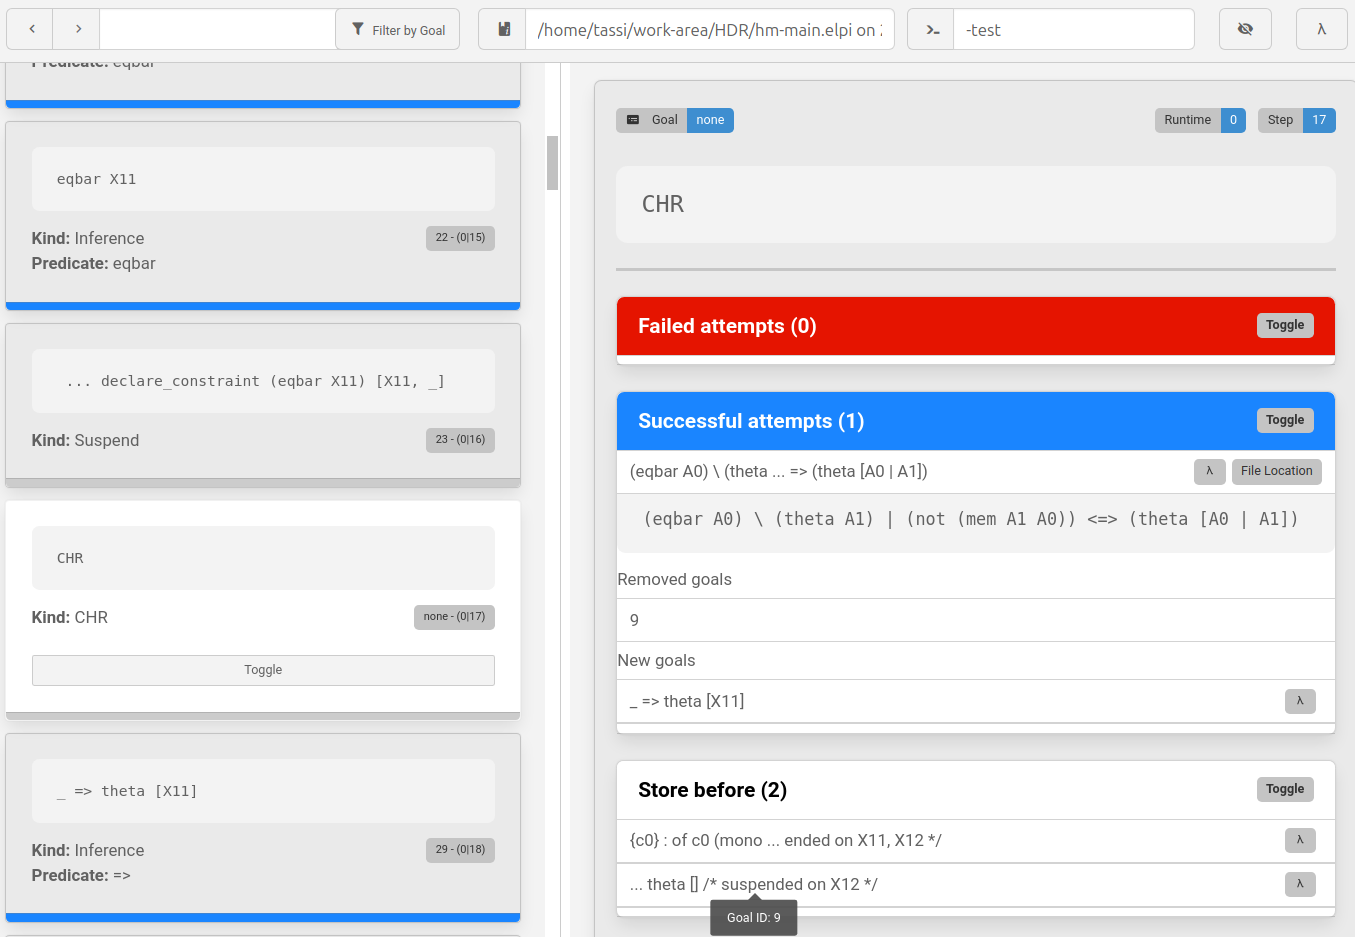
\includegraphics[width=.9\textwidth]{trace}
    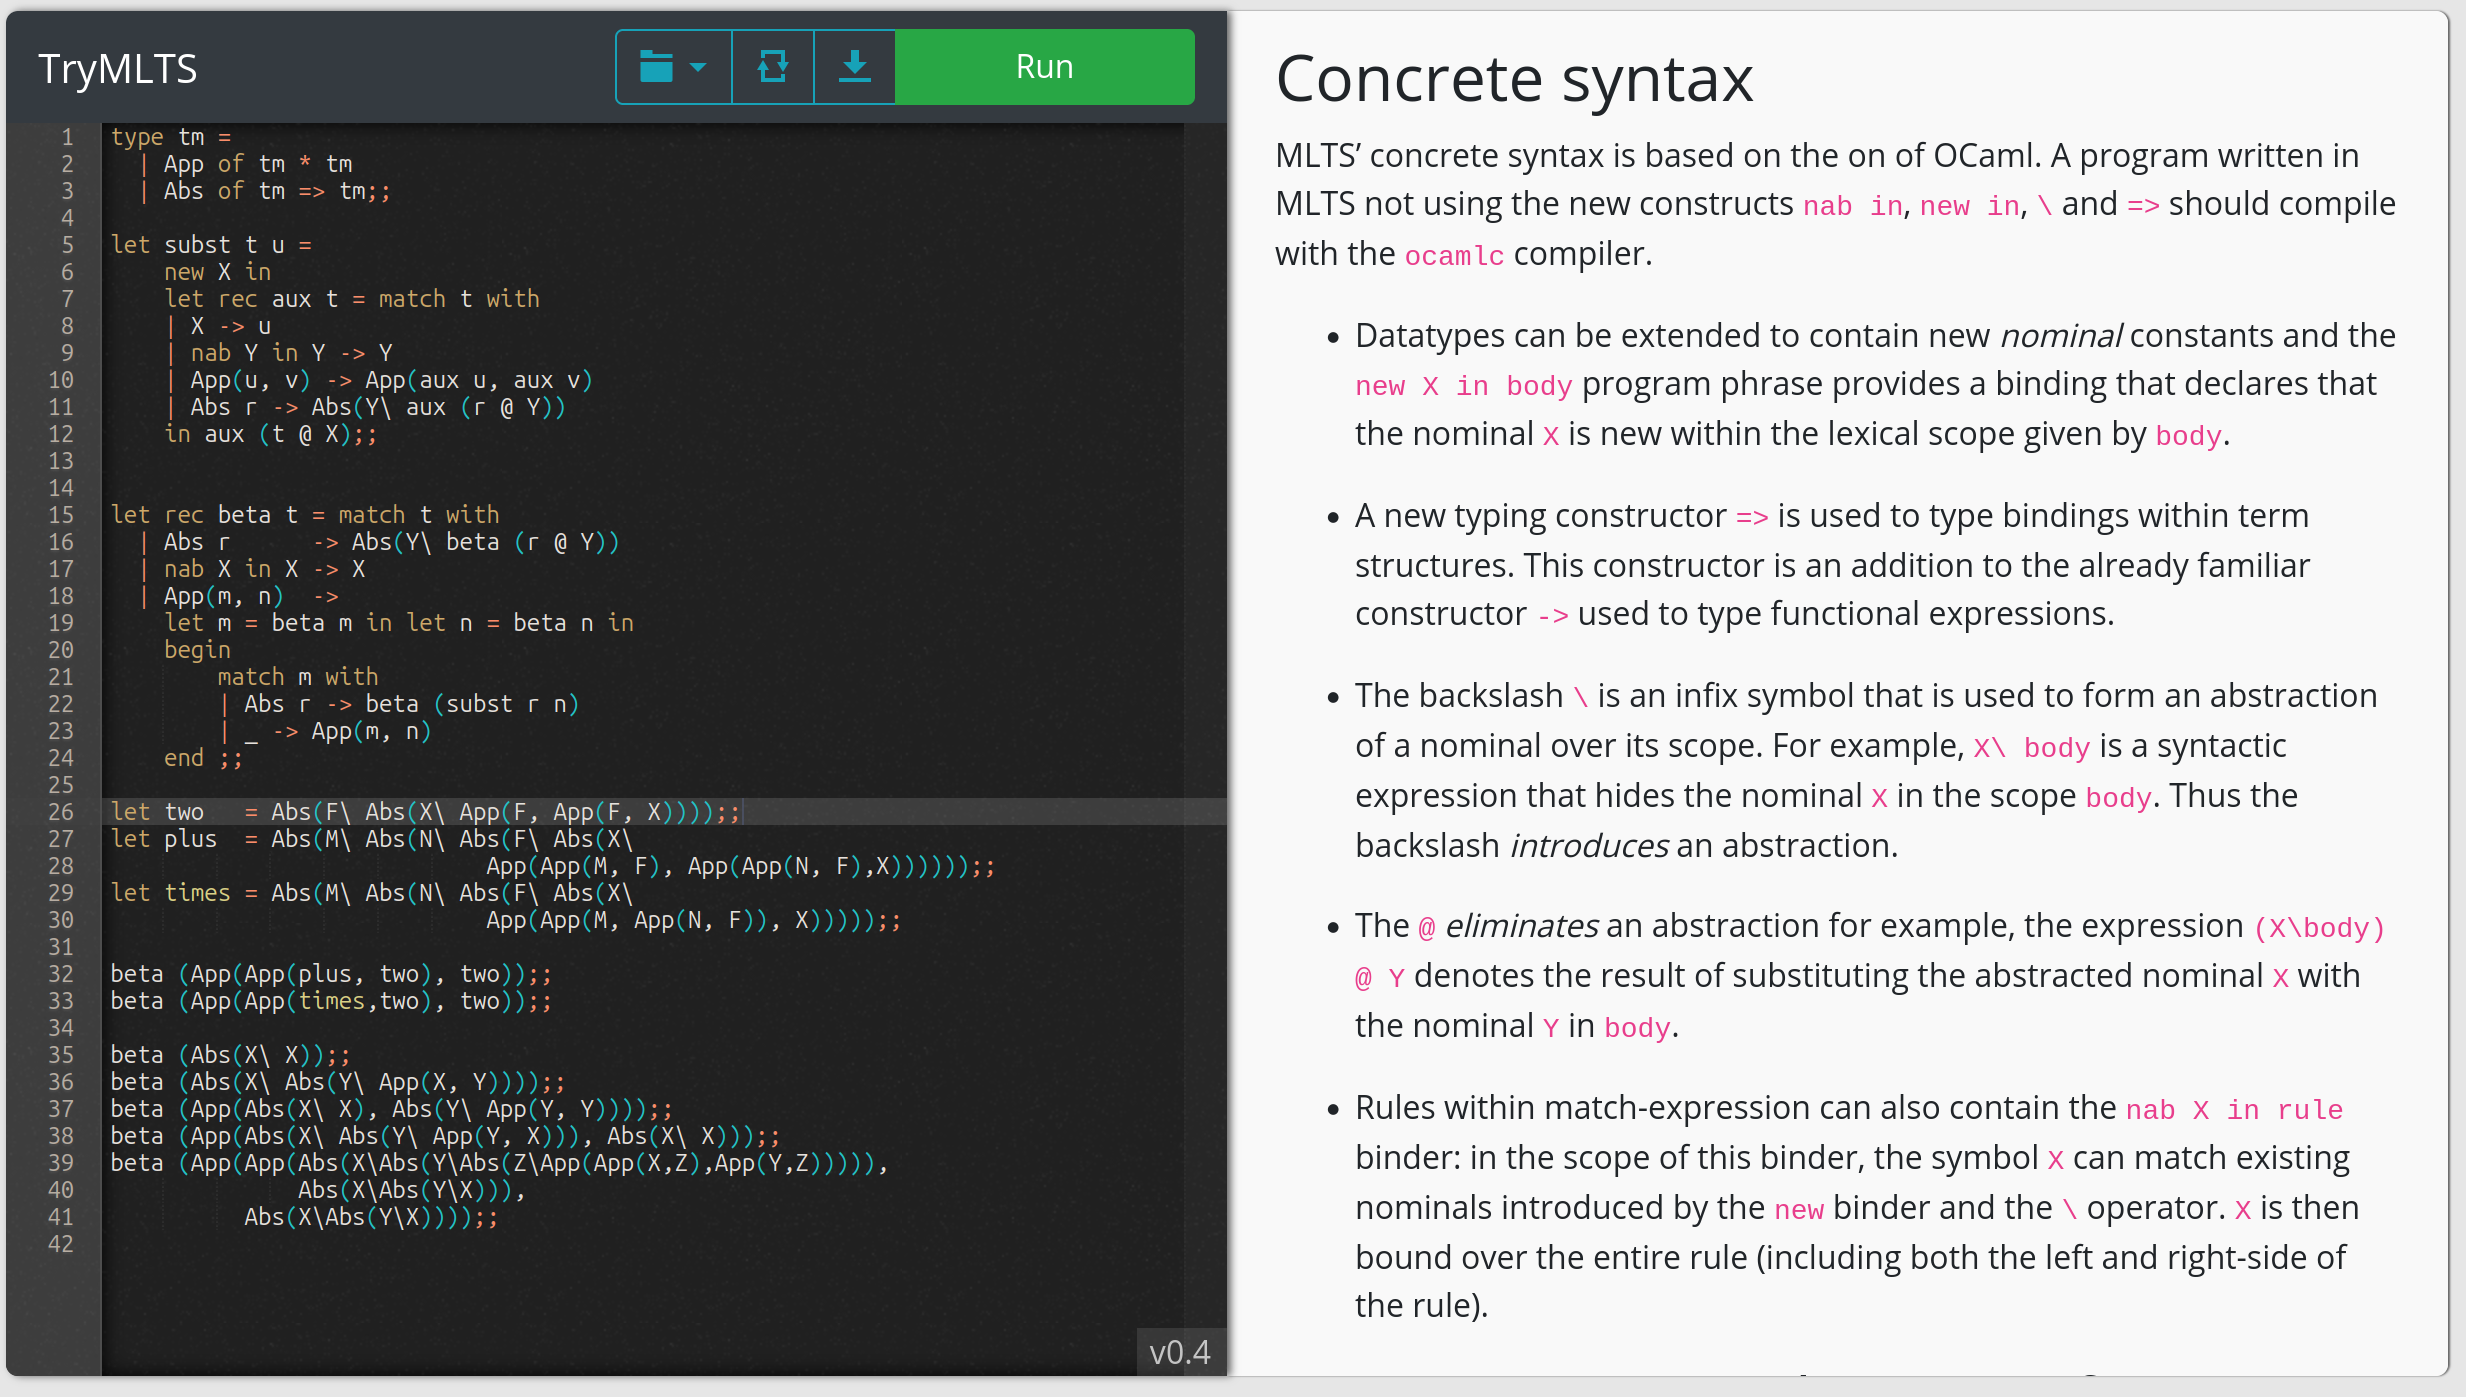
\includegraphics[width=.9\textwidth]{MLTS}
    \caption{Screenshot from \url{https://voodoos.github.io/mlts/}\label{fig:mlts}}
\end{sidewaysfigure}

\subsubsection{The role of Elpi in MLTS}

In G\'{e}rard's Ph.D., Elpi played only a technological role: being a
relatively simple, self-contained interpreter written in OCaml, Elpi could be
transpiled to a JavaScript library quite easily.

At the same time, G\'{e}rard's Ph.D. was quite inspirational to me, since
bridging the gap between the logic and functional paradigms, and bringing
automatic binder management to the latter, seems within reach thanks to his
work.


\subsection{A proof assistant for local set theory}

Nathan Guermond developed a tiny proof assistant based on a flavor of set
theory~\cite{https://doi.org/10.1112/blms/22.1.101} using
Elpi.\footnote{\url{https://github.com/nguermond/local-set-theory}}


\subsubsection{The role of Nathan Guermond in Elpi}

During the development of his proof assistant, N. Guermond discovered and
helped me fix quite a number of bugs involving $\eta$-equivalence in Elpi's
unifier. In particular, the unifier was very incomplete when dealing with
$\eta$-equivalence of non-ground terms. In a way, I feel Guermond's
experiments were more instrumental to Elpi than Elpi was to his experiment.
Thanks Nathan!

\chapter{Conclusion}

\section{Summary}


In this document, I have presented the Elpi programming language, its
implementation, and its main application as an extension language for Rocq.

\subsection{Elpi the language}

The Elpi programming language is built upon two foundational languages from the
1990s that have been extensively studied: $\lambda$Prolog and Constraint
Handling Rules (CHR). $\lambda$Prolog plays the primary role, as most Elpi
programs manipulate syntax trees with binders. CHR is essential for scaling the
programming comfort of $\lambda$Prolog to syntax trees with holes, without
burdening the language with numerous non-logical introspection features.

Throughout this document, I have emphasized that the \emph{key} feature of Elpi
is its rule-based nature. I have identified three main advantages:
\begin{enumerate}
\item Dynamic rules allow the language to scale effectively to syntax with binders (see \cref{sec:hello}).
\item Static rules make it easy to write code that is easily extensible (see \cref{sec:homo}).
\item Treating rules as code units greatly facilitates self-manipulation (see \cref{sec:tb}).
\end{enumerate}

I invite the reader to attempt writing the \rocq{to_bool} tool shown in
\cref{sec:tb} in any other extension language, and to match it in both
size and functionality.

I also wish to highlight the importance of the clarity provided by
$\lambda$Prolog (and CHR) in the design of Elpi. Building on sound foundations
draws a clear distinction between syntactic sugar and ``hacks.'' In particular,
the parallel between the execution of $\lambda$Prolog code and proof search in
intuitionistic proof theory made it evident that I should avoid 
some ad-hoc introspection primitives, such as those described in~\cite[Section 8 and
later]{10.1145/3236788}, to implement the type inference algorithm for a form
of Standard ML (see \cref{sec:milner}) or the type checker for the
simply typed $\lambda$-calculus (see \cref{sec:chrui}). The former
requires examining the typing context, i.e., the hypothetical rules of the
current goal, akin to a proof rule that inspects the proof tree of a premise.
The latter is even more complex, as it finds two (suspended) proof branches for
similar goals and, under certain conditions, joins them. Explaining these
``proof search'' steps at the meta-level at which CHR operates is possible -- even
formally -- as the meta-theory of the proof system.


\subsection{Elpi the software}


What I enjoy most about my work is designing and building
tools~\cite{DBLP:journals/jar/AspertiCTZ07,gonthier:inria-00258384,Coq-refman}.
To me, Elpi is a tool for building tools more efficiently. Implementing Elpi
was great fun; in fact, it is my first fully-fledged programming language. The
time required to produce a working implementation would have been prohibitive
without an Inria position: free from compulsory teaching duties and with
engineering support from the institute. % (see~\cref{sec:trace}).

It is also important to acknowledge that I stood on the shoulders of a
giant: Elpi is written in OCaml, which enables both good performance and
ease of integration with Rocq. The ability to use mutable data structures to
represent unification variables allows Elpi to avoid reifying the heap (the
assignment), thereby aligning the notion of garbage in Elpi data with that in
OCaml data. This makes it possible to rely on the powerful OCaml garbage
collector for Elpi. At the same time, OCaml's rich type system simplified the
development of the Foreign Function Interface in a generic way, somewhat
analogous to how the signature of printf depends on the format string.
GADTs proved to be essential for this purpose.

My main contribution to the implementation of $\lambda$Prolog is the
observation that De Bruijn levels enable an efficient implementation of a
fragment of the language~\cite{dunchev15lpar}. The fragment
$\mathcal{L}_\lambda^{\beta}$ occurs frequently in real code and supports
constant-time operations and constant-size data representation as the context
of bound variables grows in length.

\subsection{Rocq-Elpi}


At the time of writing, Elpi comprises about 20,000 lines of code:
approximately 10,000 for the runtime and 10,000 for the parser, static checker,
and compiler. Rocq-Elpi totals 13,000 lines: 5,000 for the Higher Order
Abstract Syntax (HOAS) of Rocq terms; 5,000 for the bindings of
about 300 Rocq APIs; and 3,000 for the vernacular language used to declare
programs. The most complex part is the HOAS, but it is also what makes the
language stand out, enabling each Rocq API to require, on average, only 16
lines to be exposed to Elpi (including documentation).

Unsurprisingly, its development was driven by the applications written in it,
particularly Hierarchy Builder (\cref{sec:hb}) and Derive (\cref{sec:derive}).

Rocq-Elpi was developed as an open source project from the very beginning,
keeping the Rocq development team informed of the effort. Their commitment to
providing patches to Rocq-Elpi whenever a Rocq API evolved made its development
sustainable over more than seven years. Contributions from the Rocq community
were also very important, especially from power users such as BlueRock Systems,
who contributed a substantial amount of code.

\subsection{Applications written in Elpi}

A significant number of tools for Rocq have been written in Elpi, either by
myself or by Rocq power users.

Among these, the most impactful for the Rocq community is Hierarchy Builder, as
it unblocked the development of the Mathematical Components library -- a
widely used piece of Rocq code. Its \texttt{ssreflect} component is the most widely
depended-upon Rocq package, which in turn makes Hierarchy Builder (and
Rocq-Elpi) very important parts of the Rocq ecosystem.

It is also worth mentioning the existence of a substantial amount of
closed-source Elpi code used internally by BlueRock Systems. I wish them
success in their industrial applications.

\section{Current and Future Work}

If only I had a century -- or perhaps two.

There are two main axes to consider: Elpi as a language in its own right, and
Rocq-Elpi as a framework for extending Rocq. On the Elpi side, the most
valuable improvement would be to increase its appeal to programmers already
experienced in functional languages. Most newcomers to Elpi are familiar with
functional programming and are encountering logic programming for the first
time. Improvements related to syntax -- a delicate, though not deeply
intellectual, aspect of any language -- are important. Another significant area
is static analysis, which is so prevalent in modern functional languages that
programmers often take it for granted (for example, an untyped language no
longer feels familiar, even if it is functional). On the Rocq side, it seems
reasonable to pursue deeper integration with the system, making Elpi an
integral part of Rocq. Power users frequently request a reduction in the
inevitable friction caused by a language integrated as a plugin, which is
limited by Rocq’s public extension points and extensible syntax.

Below, I discuss several concrete aspects of these two directions.

\subsection{Static Analysis and Functional Programming Languages}

Fissore integrated a determinacy checker into Elpi 3.0~\cite{elpidet}, along
with a new keyword, \elpi{func}, to be used in place of \elpi{pred} in
predicate signatures. This static check essentially guarantees that each call
to a functional predicate \elpi{p} is operationally equivalent to a call to
\elpi{once p}:

\begin{elpicode}
pred once i:pred.
once P :- P, !.
\end{elpicode}

\noindent As expected, \elpi{once} can be flagged as \elpi{func} since it
never leaves any choice points behind. The signature below uses an arrow to
separate inputs from outputs, indicating that \elpi{once} behaves as a
function operationally, i.e., it leaves no choice points even if its argument
does.

\begin{elpicode}
func once (pred) -> .
\end{elpicode}

\noindent An interesting example comes from the functional programming
repertoire:
\begin{elpicode}
func map (func A -> B), list A -> list B.
map F [] [].
map F [X|XS] [Y|YS] :- F X Y, map F XS YS.
\end{elpicode}

\noindent The signature states that \elpi{map} is a function under the
condition that its higher-order argument \elpi{F} is a function. If the
precondition is not met, \elpi{map} is considered miscalled but still runs
fine, even if it may leave choice points. Miscalled functions are tracked by
the static analyzer and treated as relations for analyzing the surrounding
code. In other words, the signature of \elpi{map} is allowed to degrade to the
following one, which requires nothing of its input but also guarantees nothing
about the choice points it may leave:
\begin{elpicode}
pred map (pred A -> B), list A -> list B.
\end{elpicode}

Since the syntax for \elpi{func} requires input arguments first, it paves the
way for a syntax for functional predicate bodies that is closer to functional
languages, where expressions and statements are intermingled. Spilling,
Section \ref{sec:spilling}, already moves in this direction, but one must
explicitly invoke it by using curly braces instead of parentheses (which can
be omitted when not needed by the parser). One wonders if this default could
be reversed for functional predicates, enabling the previous program to be
unambiguously written as follows:

\begin{elpicode}
func map (func A -> B), list A -> list B.
map F [] R :- R = [].
map F [X|XS] R :- R = [F X|map F XS].
\end{elpicode}

\noindent Currently, one has to write:
\begin{elpicode}
map F [X|XS] R :- R = [{F X}|{map F XS}].
\end{elpicode}

\noindent In turn, the \elpi{R :- R} part could be made implicit, yielding the
familiar code below:

\begin{elpicode}
func map (func A -> B), list A -> list B.
map F [] = [].
map F [X|XS] = [F X|map F XS].
\end{elpicode}

\noindent In this way, I wonder whether some syntactic sugar, driven by types
and determinacy, could recover some of the benefits of functional languages
while retaining \emph{all} the advantages of $\lambda$Prolog.
MLTS~\cite{mlts} goes in this direction, maintaining automatic binder
management but dropping the rule-based nature, and thus loosing automatic context
management and easy self-extensibility.

\subsection{Certified Runtime}

Over the years, I have gained confidence that the runtime is mostly correct,
but I would very much like to machine-check some parts.

In the past ten years, I have found and fixed four bugs that I consider
relevant (i.e., they could be triggered in legitimate code) and somewhat
embarrassing. Two were related to beta reduction: a routine used throughout
the codebase had two code paths that could sometimes be
incorrect. The root cause was a misnamed variable: \elpi{extraargs} did not
actually hold \emph{all} the extra arguments (those for which there is no
lambda), which misled the programmer into discarding some arguments. The other
two bugs consisted of bad optimizations, fortunately not very relevant in
practice, in the higher-order unification algorithm.

As Fissore and I are mechanizing~\cite{elpidet}, we have begun to take the
first steps in this direction, but I believe it would take a full Ph.D. to
complete the mechanization of a proof of correctness of the runtime.

\subsection{Program Logic for Elpi}

This is the area where even a hundred years would not suffice for me, but
there are smarter people who could tackle it. Abella~\cite{abella} is a good
starting point, as it comes with a program logic for plain $\lambda$Prolog.
This program logic does not consider the cut operator.

The big-step semantics in~\cref{sec:sem} does consider cut,
but it is not clear that it would provide a good
foundation for a program logic. In the ongoing mechanization of~\cite{elpidet},
we were forced to define an equivalent semantics with a much more explicit
description of the ongoing computation in order to reason about the scope of a
cut. While this facilitated proofs by making invariants easier to express, it
also departs from what the symbolic evaluation of a logic program looks like.
In particular, the computation state is much more complex than the list of
alternatives used in~\cref{sec:sem}. Proving the two semantics equivalent in Rocq
is ongoing work.

From a practical perspective, it is unclear to me if programs written in
Rocq-Elpi would truly benefit from a program logic. Rocq features five
extension languages to our knowledge (Ltac1, Ltac2, MTac, Meta-Rocq, and
Elpi), and only Meta-Rocq has one: it uses Gallina itself as a programming
language, so, at least in principle, one could use Rocq to prove properties of
meta-programs in Rocq itself. While I find it very intriguing intellectually,
this possibility has found, at the time of writing, almost no application. So
I'm skeptical that providing a program logic for the full Elpi language would
make it significantly more practical. Hence, it will not be a priority of
mine, but I would love to read such a program logic written on paper by
someone else.

\subsection{Elpi as a Foundational Language}

I have always seen, and still see, Elpi as a programming language that puts
\emph{practicality} before \emph{foundationality}, i.e., disregarding the
possibility of looking at Elpi programs, or their execution, as a formal
specification or formal proof.

One of the reasons is surely that I felt in the marmitte\footnote{As Obelix felt
in the pot of magic potion as a child, from the French comic Asterix.}
of the Calculus of
Inductive Constructions very early in my career, possibly because the French
and Italian schools are quite close in that respect. So, maybe unconsciously,
the foundational language has always been Rocq to me, leaving to Elpi the role of
being practical.

At the same time, my voyage in the neighborhood of computational logic gave me
the opportunity to see other ways to look at programming languages with
support for binders, i.e., as frameworks to formally describe the object of
interest and possibly reason about it. Even if I did not choose to follow the
footsteps of Twelf~\cite{twelf}, Beluga~\cite{DBLP:conf/cade/PientkaC15,10.1007/978-3-642-12251-4_1},
or MMT~\cite{RABE20131} when it comes to being a foundational language, the literature
that describes these systems has been very influential to me, and I think it is
fair to say that Elpi would not have existed without it.

\subsection{Deeper Integration in Rocq}

There are plenty of Prolog implementations in the Rocq codebase, most of which
are disguised as other features. Some tactics to automatically prove
tautologies essentially explore the search space by backtracking. Type class
resolution essentially amounts to executing a logic program~\cite{fctc}.
Canonical Structure resolution is yet another, deterministic, logic
program~\cite{tassi13}. The entire proof engine sits atop a logic programming
monad à la LogicT~\cite{logicT}.

All these parts could benefit from Elpi, or at least from some of its
implementation techniques, but it is unclear how realistic it would be to
replace them with Elpi-based alternatives in a production system such as Rocq.

As part of his Ph.D., Fissore has implemented an alternative type class solver.
It is based on an Elpi program that compiles type class instances into rules,
which are then queried each time Rocq needs to resolve a type class
instance~\cite{newtc,unifforfree}. While the approach seems promising, the
chances of completely replacing the existing engine (with all its quirks) are low.
Fissore also found it difficult to find real and computationally demanding
examples to justify the introduction of caching mechanisms such as tabling in
Elpi~\cite{selsam2020tabledtypeclassresolution,brigittePHD}. He (or we) will
probably implement a simple version of tabling in the future, but focusing on
user experience (e.g., preventing loops) rather than performance.

Pierre Roux, Quentin Vermande, and Cyril Cohen have conducted substantial
experiments leveraging Elpi in the elaboration process of Rocq, particularly
to obtain well-typed terms from intuitively correct but ill-typed ones, both
in the context of arithmetical and set-theoretic expressions. Some examples are
quite convincing, and deeper integration of Elpi in Rocq would enable the
generation of more informative error messages when these elaboration
mechanisms fail.

Finally, based on my experience implementing the first Elpi proof of concept
(\cref{sec:poc}), the Rocq proof engine could benefit from the trail mechanism
as implemented in Elpi. It turns out that, for a typical Elpi workload, mutable
terms and a trail (a log of mutable cells to unset upon backtracking) provide
much better performance than immutable terms paired with a substitution
implemented as a functional map (a reified heap, essentially). This is partly
because the OCaml garbage collector can do its job in the former case, while
the substitution grows unchecked in the latter. Reworking the proof engine to
validate this efficiency claim would require substantial engineering effort, but
could also benefit long running automation.

\subsection{Rocq as a Logical Framework}

The history of logical frameworks and interactive provers is deeply intertwined.
Perhaps the most well-known prover rooted in this idea is Isabelle, which hosts
various foundational languages, ranging from the set theory Isabelle/ZF to
first-order classical logic Isabelle/FOL and the widely recognized higher-order
logic Isabelle/HOL. However, a significant drawback in its design is that the
logical framework is so weak, from a proof-theoretic perspective, that it cannot
effectively address these formal systems. For instance, one cannot relate a
result in Isabelle/ZF with one in Isabelle/HOL, nor reuse the automatic proof
search tools that make Isabelle/HOL so practical in Isabelle/ZF. Supporting this
observation, Paulson implemented Isabelle/ZF and later mechanized ZF in
Isabelle/HOL~\cite{zfhol}.

In essence, each Isabelle/X is a distinct, incompatible prover with Isabelle/Y.
The economy achieved by sharing a common implementation infrastructure seems
minimal compared to the potential economy of sharing mechanized theorems. One
approach to address this issue is to reconcile different theories via external
translation, such as those provided by Dedukti~\cite{dedukti}. However, this
method makes it challenging to reason about the translation itself.

An emerging approach is to use Rocq's logic as the logical framework. While the
Calculus of Inductive Constructions was not explicitly designed for this
purpose -- for example, the function space is not ideal for an HOAS encoding of
terms with binders, and it is unrestricted with respect to duplication -- it still
offers a programming language, Gallina, that can encode other formal systems.
Proof-theoretically, CIC is robust enough to contain, reason about, and share
theorems across these systems. A prominent example of this approach is
Iris~\cite{10.1007/978-3-662-54434-1_26}, a separation logic proved sound in
Rocq. Thanks to its proof mode~\cite{IPM}, Iris can be used to reason about
imperative programs within Rocq. Moreover, pointers and heap locations are often
related to mathematical (immutable) objects like lists made of cons and nil via
inductive predicates. This enables imperative algorithms to be connected to
their functional specifications, allowing theorems to be shared at this level
possibly by 
a proved-correct transfer using tools like Trocq~\cite{10.1007/978-3-031-57262-3_10}.

Other examples of frameworks include VST~\cite{VST}, which implements a program
logic for C, and the FOL~\cite{FOL} library, which provides results on its
metatheory and enables proof writing within it. Even the Mathematical Component
library~\cite{assia_mahboubi_2022_7118596} follows this approach, albeit with
a thinner framework compared to the ones above. The extensive use of booleans to encode
decidable propositions in the Mathematical Component library makes reasoning by
excluded middle appear native. This approach paves the way for proof irrelevance,
effectively creating a comfortable shell for classical reasoning within CIC
without adding axioms, thereby providing a reusable base of theorems for other
frameworks. For example,~\cite{10461453} reuses linear algebra from Mathematical
Components to verify in VST the correctness of a C function that multiplies sparse
matrices over IEEE-754 conforming floating-point numbers.

If this trend continues, Elpi could play two significant roles. First, it could
continue to serve as an extension language. These frameworks require encoding,
and Elpi can assist in their implementation or abstract them for the user. For
instance,~\cite{krebbers25} provides users with the illusion of having inductive
predicates in the Iris logic. Second, and perhaps more intriguingly, the Rocq
developers could
attempt to retrofit a logical framework in CIC, inspired
by~\cite{concon}. If this happens, the techniques used to implement Elpi's
runtime could offer a solid foundation for the logical framework infrastructure
required by the new type theory.


\backmatter

%\nocite{*}
\printindex[concept]
\printbibliography[title={Our Bibliography}, keyword=me]
\printbibliography[title={Bibliography}, keyword=they]
\end{document}